% Ggf. Option "numbers=noenddot" einfügen, damit "Abbildung 3.1: _" statt "Abbildung 3.1.: _" verwendet wird.
%\documentclass[11pt, twoside, colorback, accentcolor=tud2c, nopartpage, bigchapter, fleqn, ngerman, longdoc]{tudreport}

% Das Verzeichnis iatsada zum Pfad hinzufügen, so dass \usepackage{iatsada} und die Bib-Stile funktionieren
% Sofern dies nicht vorhanden ist, wird auf das gemeinsame iat_sada_common/texmf/tex/latex/iatsada/ zurückgegriffen
% https://tex.stackexchange.com/questions/79058/can-a-default-path-be-set-globally-for-input-akin-to-graphicspath
\makeatletter
\providecommand*{\input@path}{}
\edef\input@path{{iatsada/}{../iat_sada_common/texmf/tex/latex/iatsada/}{../iat_sada_common/texmf/tex/latex/iatsada/common/logos/}{../iat_sada_common/texmf/tex/latex/biblatex-iatsada/}{../iat_sada_common/texmf/tex/latex/biblatex-iatsada/bbx/}{../iat_sada_common/texmf/tex/latex/biblatex-iatsada/cbx/}{../iat_sada_common/texmf/tex/latex/abk/}{../iat_sada_common/texmf/tex/latex/ifclass/}{../iat_sada_common/texmf/tex/latex/uniinput/}\input@path}% prepend
\makeatother

% =================================================================================
% Hier auswählen, ob Abgabeversion für TUbama oder nicht
% =================================================================================
\newif\ifSADATUbama
\SADATUbamatrue					% Abgabeversion für TUbama (PDF/A)
\SADATUbamafalse				% keine Abgabeversion

\newcommand{\selectMainLanguage}{\selectlanguage{ngerman}} % Wenn die Arbeit auf deutsch geschrieben wird
%\newcommand{\selectMainLanguage}{\selectlanguage{english}} % Wenn die Arbeit auf englisch geschrieben wird

% =================================================================================
% Ausnahmen von der automatischen Silbentrennung
% =================================================================================
\hyphenation{Aktu-ali-sie-rung Screen-shots Pa-rallel-ro-bo-ter Zu-stands-raum-mo-del-le nach-voll-zieh-bar Pro-jekt-se-mi-nar}
% =================================================================================

% =================================================================================
% Hier auswählen, ob TUD-Design oder nicht
% =================================================================================
\newif\ifTUDdesign
\TUDdesigntrue					% TUD-Design
%\TUDdesignfalse				% Für Rechner ohne installierte TUDdesign-Pakete
% =================================================================================

% =================================================================================
% Hier NICHTS ändern!
% =================================================================================
\ifSADATUbama
	\input{./common/metadata.tex}
\fi
\ifTUDdesign
	% Ggf. Option "numbers=noenddot" einfügen, damit "Abbildung 3.1: _" statt "Abbildung 3.1.: _" verwendet wird.
	\documentclass[11pt, twoside, colorback, accentcolor=tud2c, nopartpage, bigchapter, fleqn, ngerman, longdoc]{tudreport}
\else
	\documentclass[11pt, a4paper, twoside, fleqn, ngerman]{scrreprt}% Für Entwurf auf Rechnern ohne installierte TUDdesign-Pakete
	\usepackage{exscale}% Korrektur math-Zeichen
	\usepackage{eurosym}
\fi
% Dieses File dient zum Einbinden wichtiger und nützlicher Pakete.
% Nicht alle Pakete müssen verwendet werden.
%
\usepackage[T1]{fontenc}	% Für Silbentrennung bei Wörten mit Sonderzeichen (z.B. Umlaute)
\usepackage[utf8]{inputenc}	% Um Sonderzeichen (ä, ß, é, ...) direkt eingeben zu können
\usepackage[english,main=ngerman]{babel}
							% Für Sprachenspezifisches
							% ngerman ist schon als globale Option definiert
\usepackage{ifclass}
\usepackage{iflang}			% für sprachabhängige Einstellungen
\usepackage{xkvltxp}		% für Macros in key-value Paketoptionen

%\usepackage{helvet}		% Helvetica als Standard-Sans-Schriftart
\usepackage[stable]{footmisc}
\usepackage{booktabs}


\usepackage{graphicx}		% zum Einbinden von Postscript
\usepackage{psfrag}			% Beschriftung der Bilder
\ifbeamer
	\usepackage{amsmath}% Mehr mathematischer Formelsatz
\else
	\usepackage[tbtags]{amsmath}% Mehr mathematischer Formelsatz
\fi
%\usepackage{amssymb}		% Mehr mathematische Symbole
%\usepackage{amsthm}

\usepackage{float}			% Für Parameter [H] bei Fließobjekten

\usepackage{epsfig}			% Um eps-Bilder einzubinden
\usepackage{scrhack}		% Um Warnung "float@addtolists detected" zu unterdrücken 
\usepackage{subcaption}		% Für Unterabbildungen
\usepackage{ltxtable} 		% Vereinigt TabularX und Longtable
\usepackage{upgreek}		% Für nicht-kursive kleine griechischen Buchstaben
\usepackage{uniinput}		% Diverse Makros zum Ersetzen von UTF8 Zeichen durch Latex äquivalente					
\usepackage{multirow}		% Für mehrzeilige Felder in Tabellen
\usepackage{rotating}		% Zum Drehen von Objekten
\usepackage{icomma}			% Damit nach Dezimalkommas kein Abstand eingefügt wird
\usepackage{dcolumn}		% Zum Ausrichten von Tabellenspalten am Dezimaltrennzeichen

%\usepackage{wrapfig}		% Für kleine Bilder am Rand
%\usepackage{floatflt}		% Alternative zu wrapfig
%\usepackage[hang]{caption}	% Damit mehrzeilige Bildunterschriften gut aussehen
\usepackage{textcomp}		% Für Sonderzeichen im normalen Text
							% (offensichtlich in tudreport schon eingebunden)
\usepackage[ngerman]{varioref}		% Für vref
\usepackage{color}			% Für farbigen Text
\usepackage{placeins}		% Für \FloatBarrier
\usepackage{xspace}
\usepackage{cancel}			% Zum Wegstreichen von Gleichungstermen \cancel{a} oder \cancelto{0}{a}
\usepackage{listings}		% Um formatierten Quellcode einzubinden


\usepackage{array}			% Für Zellentyp "m{}" in tabular-Umgebungen (Vertikal zentriert)
\usepackage{moreverb}		% Für Umgebung "`verbatimtab"' (Verbatim mit Tabs)
\renewcommand{\verbatimtabsize}{4\relax}	% Standardtabweite in "`verbatimtab"'
											% ist 4 Zeichen

\usepackage{abk}

\usepackage{siunitx}		% Um Zahlen mit Einheiten korrekt darzustellen \SI{12}{\meter\per\second} 
\sisetup{
	range-units=single,
	range-phrase={\,\textnormal{\textendash}\,},
	output-decimal-marker={,},
	%per-mode=fraction,
	per-mode=reciprocal,
	per-mode=symbol,
	math-micro=\muup,% Im TU-Design passt das µ sonst nicht
	math-ohm  =\Omegaup,
	text-micro={\fontfamily{mdbch}\textmu},
	text-ohm  ={\fontfamily{mdbch}\textohm}
}

% ======== Glossar =========
\newif\ifSADAuseglossaries
\SADAuseglossariestrue
\SADAuseglossariesfalse
\ifSADAuseglossaries
	\usepackage[automake, acronym, symbols, toc, translate=babel]{glossaries}
	\addto\captionsngerman{%
		\renewcommand*{\acronymname}{Abkürzungsverzeichnis}
		\renewcommand*{\glssymbolsgroupname}{Symbolverzeichnis}
	}
\fi

% ======== Anfang Literaturverwaltung =====
%\usepackage[datename]{babelbib}	% Für deutsche Literaturverwaltung
%\setbtxfallbacklanguage{ngerman}
%\btxprintISSN{false}
%\setbibliographyfont{lastname}{\textsc}%
\usepackage[babel]{csquotes}
\ifbeamer
	\usepackage[
		backend=biber,
		style=iatsada-numeric,
		backref=false
	]{biblatex}					% Für deutsche Literaturverwaltung
\else
	\usepackage[
		backend=biber,
		style=iatsada-numeric,
		backref=true
	]{biblatex}					% Für deutsche Literaturverwaltung
	% ==========================================
\fi

\ifbeamer
	% Hier Pakete die nur für Präsentationen benötigt werden
	\usepackage{animate}
	\usepackage{multimedia}
\fi

\ifbeamer
	\usepackage{todonotes}		% Für Anmerkungen \todo{Bitte ändern} bzw. \todo[inline]{Bitte ändern}
\else
	\usepackage[textwidth=1.8cm, textsize=tiny]{todonotes}		% Für Anmerkungen \todo{Bitte ändern} bzw. \todo[inline]{Bitte ändern}	
	%muss eigentlich hinter begin{document} stehen, macht dann aber die Fusszeile kaputt
	%\setlength{\marginparwidth}{1.8cm} % notwendig damit todos am Rand korrekt dargestellt werden (siehe Doku todonotes Paket)
\fi

% Das Packet hyperref immer als letztes einbinden (nur bookmark darf danach kommen)!
% Für Verlinkungen im erzeugten pdf
\ifbeamer
	\usepackage[colorlinks=false]{hyperref}
\else
	\usepackage[unicode=true, colorlinks=false, breaklinks=true]{hyperref}
	\ifSADATUbama
		\usepackage[a-1b]{pdfx}
	\fi
\fi
\usepackage{bookmark}			% verwendete Pakete einbinden
\input{common/setup/pgfsetup.tex}			% Alles was mit tikz und pgf zu tun hat
% Diese Datei dient zum definieren nützlicher Befehle.
% Sie soll lediglich als Beispiel dienen, wie Befehle definiert werden, und welche Befehle nützlich sein können.
\newcommand{\eqp}{\ensuremath{\, \, \, .}}
\newcommand{\M}[1]{\textbf{#1}} %Matrix  M
\newcommand{\Mr}[1]{\textbf{#1}_\rho} %Matrix mit tiefgestelltem rho, M_rho
\newcommand{\Mtil}[1]{\tilde{\textbf{#1}}} %Matrix mit Tilde
\newcommand{\Mtilt}[2]{\tilde{\textbf{#1}}_{#2}} %Matrix mit Tilde mit tiefgestelltem arg2
\DeclareRobustCommand{\Mt}[2]{\textbf{#1}_{#2}} %Matrix M mit tiefgestelltem arg2


\DeclareRobustCommand{\w}[1]{\underline{#1}} %Vektor arg1 unterstrichen 
\DeclareRobustCommand{\wt}[2]{\underline{#1}_{#2}} %Vektor unterstrichen w mit tiefgestelltem arg2
\DeclareRobustCommand{\wr}[1]{\underline{#1}_{\rho}} %Vektor unterstrichen mit rho, w_rho

% Inhalt
% ======
%	Makros für Referenzen (Abbildungen, Zitate, ...)
%	Makros für Abbildungen
%	Makros für Einheiten, Exponenten
%	Makros für Formeln
%	Makros für Entwurf
%   Definitionen für Umgebungen

% Makros für Abbildungen
% ======================
	% zum Skalieren nach Ersetzen durch psfrag
	\newcommand*{\incgraphicsw}[2]{\resizebox{#1}{!}{\includegraphics{#2}}}


% Textbausteine
% =============
	% Produktnamen
	\newcommand*{\Matlab}{\textsc{Matlab}}
	\newcommand*{\Matlabreg}{\textsc{Matlab}\textsuperscript{\tiny \textregistered}}
	\newcommand*{\MatSim}{\textsc{Matlab/Simulink}}
	\newcommand*{\Simulink}{\textsc{Simulink}}
	\newcommand*{\Simulinkreg}{\textsc{Simulink}\textsuperscript{\tiny \textregistered}}
	
	% Das Makro |\name|\marg{person} formatiert einen Personennamen bspw. eines Erfinders oder Entdeckers gemäß |\name{Euler}| \arrow\ \name{Euler}.
	\newcommand*{\name}[1]{\textsc{#1}}



% Makros für Einheiten, Exponenten
% ================================

	\newcommand*{\unit}[1]{\ensuremath{\mathrm{#1}}}
	
	% Wert mit Einheit (mit kleinem Leerzeichen dazwischen), aus Text- UND Math-Modus
	\newcommand*{\valunit}[2]{\ensuremath{#1\,\mrm{#2}}}


	% "°C", im Text- oder Mathe-Modus
	\newcommand*{\degC}{
		\ifmmode
			^\circ \mrm{C}%
		\else
			\textdegree C%
		\fi}

	\newcommand*{\degree}{
		\ifmmode
			^\circ%
		\else
			\textdegree%
		\fi}
	
	% Für Exponentenschreibweise ( Anwendung: 123\E{3} )
	\newcommand*{\E}[1]{\ensuremath{\cdot 10^{#1}}}
	
	\newcommand*{\eexp}[1]{\ensuremath{\mathrm{e}^{#1}}}
	\newcommand*{\iu}{\ensuremath{\mathrm{j}}}

	\newcommand*{\todots}{\ensuremath{,\,\hdots,\,}}


% Makros für Formeln
% ==================

	% Definition für Vektor und Matizen
    \newcommand*{\mat}[1]{{\ensuremath{\boldsymbol{\mathrm{#1}}}}}
    \newcommand*{\ma}[1]{{\ensuremath{\boldsymbol{\mathrm{#1}}}}}
    \newcommand*{\mas}[1]{\ensuremath{\boldsymbol{#1}}}
    \newcommand*{\ve}[1]{\ensuremath{\boldsymbol{#1}}}
    \newcommand*{\ves}[1]{\ensuremath{\boldsymbol{\mathrm{#1}}}}

	\newcommand*{\AP}{\ensuremath{\mathrm{AP}}}
	\newcommand*{\doti}{\ensuremath{(i)^\cdot}}
	
	\newcommand*{\inprod}[2]{\ensuremath{\langle #1,\,#2 \rangle}}
	
	\newcommand*{\ul}[1]{\underline{#1}}

	% gerades "d" (z.B. für Integral)
	\newcommand*{\ud}{\ensuremath{\mathrm{d}}}
	
	% normaler Text in Formeln
	\newcommand*{\tn}[1]{\textnormal{#1}}
	
	% nicht-kursive Schrift in Formeln
	\newcommand*{\mrm}[1]{\ensuremath{\mathrm{#1}}}
	
	% gerades "T" für Transponiert
	\newcommand*{\transp}{\ensuremath{\mathrm{T}}}
	
	% gerades "rg"
	\newcommand*{\rang}{\ensuremath{\operatorname{rg}}}

	% Für geklammerte Ausdrücke mit Index (Subscript)
	% (einmal mit kursiven Index, einmal mit geradem Index)
	\newcommand*{\grpsb}[2]{\ensuremath{\left(#1\right)_{#2}}}
	\newcommand*{\grprsb}[2]{\ensuremath{\left(#1\right)_{\mathrm{#2}}}}

	% Ableitungen und Integrale
		% "normale" Ableitung (mit geraden "d"s)
		\newcommand*{\normd}[2]{\ensuremath{\frac{\mathrm{d}#1}{\mathrm{d}#2}}}
		\newcommand*{\normdat}[3]{\ensuremath{\left.\frac{\mathrm{d} #1}{\mathrm{d} #2}\right|_{#3}}}
	
		% Materielle Ableitung
		\newcommand*{\matd}[2]{\ensuremath{\frac{\mathrm{D} #1}{\mathrm{D} #2}}}
		\newcommand*{\matdat}[3]{\ensuremath{\left.\frac{\mathrm{D} #1}{\mathrm{D} #2}\right|_{#3}}}
	
		% Partielle Ableitung
		\newcommand*{\partiald}[2]{\ensuremath{\frac{\partial #1}{\partial #2}}}
		\newcommand*{\partialdat}[3]{\ensuremath{\left.\frac{\partial #1}{\partial #2}\right|_{#3}}}
	
	
	% Transformationen
	\newcommand*{\FT}[1]{\ensuremath{\mathfrak{F}\left\{#1\right\}}}
	\newcommand*{\FTabs}[1]{\ensuremath{\left|\mathfrak{F}\left\{#1\right\}\right|}}
	\newcommand*{\IFT}[1]{\ensuremath{\mathfrak{F}^{-1}\left\{#1\right\}}}
	\newcommand*{\DFT}[1]{\ensuremath{\mathrm{DFT}\left\{#1\right\}}}
	\newcommand*{\DFTabs}[1]{\ensuremath{\left|\mathrm{DFT}\left\{#1\right\}\right|}}
	\newcommand*{\Laplace}[1]{\ensuremath{\mathfrak{L}\left(#1\right)}}
	\newcommand*{\InvLaplace}[1]{\ensuremath{\mathfrak{L^{-1}}\left(#1\right)}}
	\newcommand*{\invtrans}{\ensuremath{\quad\bullet\!\!-\!\!\!-\!\!\circ\quad}}
	\newcommand*{\trans}{\ensuremath{\quad\circ\!\!-\!\!\!-\!\!\bullet\quad}}


	\newcommand*{\mlfct}[1]{\texttt{#1}}
	\newcommand*{\mlvar}[1]{\texttt{#1}}


	% Manche textcomp-Zeichen funktionieren mit dem TU-Design nicht, diese können dann mit diesem
	% Befehl gesetzt werden.
	\newcommand*{\textcompstdfont}[1]{{\fontfamily{cmr} \fontseries{m} \fontshape{n} \selectfont #1}}
	


% =================================================================================
% Defintionen für Mathe-Umgebungen
% =================================================================================
	
\ifcsmacro{theorem}{}{
	\newtheorem{theorem}{Satz}
}
\ifcsmacro{lemma}{}{
	\newtheorem{lemma}[theorem]{Lemma}	% Selber Zähler wie theorem
}
\ifcsmacro{definition}{}{
	\newtheorem{definition}{Definition}
}
% =================================================================================


% =================================================================================
% Defintionen für Beispiel-Umgebung
% =================================================================================
\makeatletter
\ifx\c@chapter\undefined
	\newcounter{chapter}
\fi
\ifx\c@examplenumber\undefined
	\newcounter{examplenumber}[chapter]% Neuer Counter bspnummer nummeriert nach Kapitel
\fi
\makeatother
\def\theexamplenumber{\thechapter.\arabic{examplenumber}}

\ifcsmacro{example}{}{
	\newenvironment{example}[1][]
	{\vskip 3\parskip plus 1pt minus 1pt \refstepcounter{examplenumber}
	\vspace{.3cm} \begin{addmargin}[1cm]{0cm} \noindent \textbf{Beispiel \theexamplenumber}: \textbf{#1}\par}
	{\end{addmargin} \par \vspace{.3cm}}
}

% Alternative, einfachere Beispielumgebung:
% \newtheorem{example}{Beispiel}
% =================================================================================

% =================================================================================
% Definitionen für Tabellen
% =================================================================================
% Spaltenstil zum Ausrichten von Zahlen am Dezimaltrennzeichen
\newcolumntype{d}[1]{D{.}{,}{#1}}


% =================================================================================
% Definitionen für Listingsumgebung
% =================================================================================

\lstloadlanguages{Matlab}

\lstdefinestyle{Matlab_colored_smallfont}{
	language = Matlab,
	keywords = {break,case,catch,continue,class,else,elseif,end,enumeration,for,function,global,if,methods,otherwise,persistent,properties,return,switch,try,while},
	tabsize = 4,
	framesep = 3mm,
	frame=tb,
	classoffset = 0,	
	basicstyle = \footnotesize\ttfamily,
	keywordstyle = \bfseries\color[rgb]{0,0,1},
	commentstyle = \itshape\color[rgb]{0.133,0.545,0.133},
	stringstyle = \color[rgb]{0.627,0.126,0.941},
	extendedchars = true,
	breaklines = true,
	prebreak = \textrightarrow,
	postbreak = \textleftarrow,
	%escapeinside = {(*@}{@*)},
	%moredelim = [s][\itshape\color[rgb]{0.5,0.5,0.5}]{[.}{.]},
	numbers = left,
	numberstyle = \tiny,
	stepnumber = 5
}

\lstdefinestyle{Matlab_colored}{
	language = Matlab,
	keywords = {break,case,catch,continue,class,else,elseif,end,enumeration,for,function,global,if,methods,otherwise,persistent,properties,return,switch,try,while},
	tabsize = 4,
	framesep = 3mm,
	frame=tb,
	classoffset = 0,	
	basicstyle = \ttfamily,
	keywordstyle = \bfseries\color[rgb]{0,0,1},
	commentstyle = \itshape\color[rgb]{0.133,0.545,0.133},
	stringstyle = \color[rgb]{0.627,0.126,0.941},
	extendedchars = true,
	breaklines = true,
	prebreak = \textrightarrow,
	postbreak = \textleftarrow,
	%escapeinside = {(*@}{@*)},
	%moredelim = [s][\itshape\color[rgb]{0.5,0.5,0.5}]{[.}{.]},
	numbers = left,
	numberstyle = \tiny,
	stepnumber = 5
}


\lstdefinestyle{C_colored_smallfont}{
	language=C,
	tabsize = 4,
	framesep = 3mm,
	frame=tb,	
	classoffset = 0,	
	basicstyle = \footnotesize\ttfamily,
	keywordstyle = \bfseries\color[rgb]{0,0,1},
	commentstyle = \itshape\color[rgb]{0.133,0.545,0.133},
	stringstyle = \color[rgb]{0.627,0.126,0.941},
	extendedchars = true,
	breaklines = true,
	prebreak = \textrightarrow,
	postbreak = \textleftarrow,
	%escapeinside = {(*@}{@*)},
	%moredelim = [s][\itshape\color[rgb]{0.5,0.5,0.5}]{[.}{.]},
	numbers = left,
	numberstyle = \tiny,
	stepnumber = 5
}

\lstdefinestyle{C_colored}{
	language=C,
	tabsize = 4,
	framesep = 3mm,
	frame=tb,
	classoffset = 0,	
	basicstyle = \ttfamily,
	keywordstyle = \bfseries\color[rgb]{0,0,1},
	commentstyle = \itshape\color[rgb]{0.133,0.545,0.133},
	stringstyle = \color[rgb]{0.627,0.126,0.941},
	extendedchars = true,
	breaklines = true,
	prebreak = \textrightarrow,
	postbreak = \textleftarrow,
	%escapeinside = {(*@}{@*)},
	%moredelim = [s][\itshape\color[rgb]{0.5,0.5,0.5}]{[.}{.]},
	numbers = left,
	numberstyle = \tiny,
	stepnumber = 5
}

% Unterstützung von Umlauten in listings und tcblistings (tcolorbox Paket)
\lstset{
	inputencoding=utf8,
	extendedchars=true,
	literate=%
		{á}{{\'a}}1
		{é}{{\'e}}1
		{í}{{\'i}}1
		{ó}{{\'o}}1
		{ú}{{\'u}}1
		{Á}{{\'A}}1
		{É}{{\'E}}1
		{Í}{{\'I}}1
		{Ó}{{\'O}}1
		{Ú}{{\'U}}1
		{à}{{\`a}}1
		{è}{{\`e}}1
		{ì}{{\`i}}1
		{ò}{{\`o}}1
		{ù}{{\`u}}1
		{À}{{\`A}}1
		{È}{{\'E}}1
		{Ì}{{\`I}}1
		{Ò}{{\`O}}1
		{Ù}{{\`U}}1
		{ä}{{\"a}}1
		{ë}{{\"e}}1
		{ï}{{\"i}}1
		{ö}{{\"o}}1
		{ü}{{\"u}}1
		{Ä}{{\"A}}1
		{Ë}{{\"E}}1
		{Ï}{{\"I}}1
		{Ö}{{\"O}}1
		{Ü}{{\"U}}1
		{â}{{\^a}}1
		{ê}{{\^e}}1
		{î}{{\^i}}1
		{ô}{{\^o}}1
		{û}{{\^u}}1
		{Â}{{\^A}}1
		{Ê}{{\^E}}1
		{Î}{{\^I}}1
		{Ô}{{\^O}}1
		{Û}{{\^U}}1
		{œ}{{\oe}}1
		{Œ}{{\OE}}1
		{æ}{{\ae}}1
		{Æ}{{\AE}}1
		{ß}{{\ss}}2
		{ç}{{\c c}}1
		{Ç}{{\c C}}1
		{ø}{{\o}}1
		{å}{{\r a}}1
		{Å}{{\r A}}1
		{€}{{\EUR}}1
		{£}{{\pounds}}1
}

		% oft verwendete Befehle aus RTM Vorlage
\input{common/macros/mymacros.tex}			% Eigene Befehle
% verwendete Pakete einbinden
\addbibresource{./bib/literature.bib}% Bibliographie einbinden
\ifSADAuseglossaries
	\makeglossaries
	\loadglsentries{./Glossar/Verzeichnisse.tex}%Glossar einbinden
\fi
\usepackage{placeins}
\usepackage[stable]{footmisc}
\usepackage{mathtools}
\usepackage{mathptmx}
\usepackage[percent]{overpic} 
\usepackage{rotating}
\usepackage{todonotes}
\usepackage{ifthen}
\usepackage{subcaption}
\usepackage{multicol}
\usepackage{pdfpages}
\usepackage{tikz}
\usepackage{graphicx}
\usepackage{pgfplots}
\usepackage{subcaption}
\usepackage{transparent}
\usepackage{listings}
\usepackage{amsmath}
\usepackage{makecell}
\usetikzlibrary{external}
\tikzexternalize[prefix={cache/}]
\usetikzlibrary{shapes, arrows, patterns}
\usetikzlibrary{decorations.pathreplacing, decorations.pathmorphing}
\usetikzlibrary{shapes.geometric}
\makeatletter
\newcommand{\myunderbrace}[2]{\settowidth{\bracewidth}{$#1$}#1\hspace*{-1\bracewidth}\smash{\underbrace{\makebox{\phantom{$#1$}}}_{#2}}}
\newcommand\MyLBrace[2]{%
	\left.\rule{0pt}{#1}\right\}\text{#2}}
\renewcommand*\env@matrix[1][*\c@MaxMatrixCols c]{%
	\hskip -\arraycolsep
	\let\@ifnextchar\new@ifnextchar
	\array{#1}}
\pgfdeclarepatternformonly[\LineSpace]{my north east lines}{\pgfqpoint{-1pt}{-1pt}}{\pgfqpoint{\LineSpace}{\LineSpace}}{\pgfqpoint{\LineSpace}{\LineSpace}}%
{
	\pgfsetcolor{\tikz@pattern@color}
	\pgfsetlinewidth{0.4pt}
	\pgfpathmoveto{\pgfqpoint{0pt}{0pt}}
	\pgfpathlineto{\pgfqpoint{\LineSpace + 0.1pt}{\LineSpace + 0.1pt}}
	\pgfusepath{stroke}
}
\makeatother

\newdimen\LineSpace
\tikzset{
	line space/.code={\LineSpace=#1},
	line space=10pt
}

% =================================================================================
% Hier Daten für studentische Arbeit eingeben
% =================================================================================
%\newcommand*{\SADATyp}{Masterarbeit}
\newcommand*{\SADATitel}{Automatisierte Luftbetankung von Passagierflugzeugen}
%\newcommand*{\SADASubTitel}{Untertitel, der bei Abschlussarbeiten ignoriert wird}
%\newcommand*{\SADASubSubTitel}{Untertitel der ebenfalls ignoriert wird}
\newcommand*{\SADAStadt}{Darmstadt}
\newcommand*{\SADAAutor}{Markus Amann, Lukas Nevermann, Matheus Schelp Langendyk, Jinyuan Zhang} % Kommagetrennte Liste der Autoren
\newcommand*{\SADABetreuerI}{Philipp Schaub, M.Sc.}
%\newcommand*{\SADABetreuerII}{\DiplIng{} Hans Hilflos}
\newcommand*{\SADABetreuerIII}{}
\newcommand*{\SADABegin}{01. November 2020}
\newcommand*{\SADAAbgabe}{15. März 2021}
\newcommand*{\SADASeminar}{09. April 2021}


\usepackage[
  % TUDmargin=true,    % Wenn ein Breiter Rand für Korrekturen gewünscht ist
	onlycolorfront=true, % Wenn nur die erste Seite einen farbigen Balken erhalten soll
	fachgebiet=RTM,      % RTM / RTP
	fachbereich=18,      % 18 / 16
	typ=PS,              % MA=Masterarbeit  BA=Bachelorarbeit PS=Projektseminar PR=Proseminar SA=Studienarbeit DA=Diplomarbeit  
	                     % script=Skript exercise=Übung report=Bericht internship=Praktikumsbericht  user=Eigener Typ, der mit \newcommand*{\SADATyp}{MeinTyp} gesetzt werden kann
	accentcolor=tud2c,   % Wird bei der automatischen Farbumschaltung verwendet.
	tikzexternal=none	 % none=keine Externalisierung, make=IAT Externalisierung, tikz=tikzexternalize
]{iatsada}

\ifcsname setcooperationlogo\endcsname
	\setcooperationlogo[height]{./Bilder/Firmenlogo}% Bei Bedarf kann ein Firmenlogo gesetzt werden, wenn tudthesis entsprechend gepatcht wurde
\fi
\setkeysinputtikz{path=./Bilder/, errorlevel=warning}
\iatsadatikzexternalmode{tikz}{
	\tikzexternalize[shell escape=-enable-write18]%tikzexternal aktivieren
}{}


% =================================================================================
% Texte für die Rückseite des Titelblatts vorgeben
% =================================================================================
\uppertitleback{}
\lowertitleback{}
\dedication{}
% =================================================================================
% Hier beginnt das eigentliche Dokument
% =================================================================================


% =================================================================================
% kann nach Ersetzung der Hilfetexte gelöscht werden
% =================================================================================
\usepackage{forest}
\definecolor{folderbg}{RGB}{124,166,198}
\tikzset{
	folder/.pic={
		\filldraw[draw={rgb:red,110;green,144;blue,169},top color=folderbg!50,bottom color=folderbg]
		(-4.2pt,5.8pt) rectangle ++(3pt,-5.8pt);
		\filldraw[draw={rgb:red,110;green,144;blue,169},top color=folderbg!50,bottom color=folderbg]
		(-4.6pt,-4pt) rectangle (4.6pt,4pt);
	}
}
\newcommand*{\Miktex}{\textsc{MiKTeX}\xspace}
\newcommand*{\texlive}{\textsc{texlive}\xspace}
\newcommand{\Texstudio}{\textsc{TeXStudio}\xspace}
\newcommand{\Texniccenter}{\textsc{TeXnicCenter}\xspace}
\newcommand{\Sumatra}{\textsc{Sumatra}\xspace}
\newcommand*{\zitat}[1]{\glqq{}#1\grqq{}}
% =================================================================================
\begin{document}
	\selectMainLanguage
\SADAmaketitle
\pagenumbering{roman}	% Bis zum Hauptteil werden römische Seitenzahlen verwendet
\SADAfirstpage

\ifSADAfinal% Aufgabestellung nur in der Abgabeversion einbinden
	% =================================================================================
	% Spezielle Seiten für studentische Arbeiten
	% =================================================================================
	\cleardoublepage
	\section*{Aufgabenstellung}

Nach einer Studie der Zürcher Hochschule für Angewandte Wissenschaften (ZHAW) aus dem Jahr 2015 \footnote{ZHAW, „Fliegende Tankstellen könnten den Luftverkehr revolutionieren“, https://www.zhaw.ch/de/medien/
	medienmitteilungen/detailansicht-medienmitteilung/event-news/fliegende-tankstellen-koennten-den-luftverkehr-revolutionieren/, abgerufen 5.10.2020} können durch Luftbetankung im zivilen Luftverkehr erhebliche Mengen an Treibstoff eingespart werden.

Um den Zusatzaufwand für Piloten möglichst gering zu halten, soll in diesem Projektseminar ein Konzept zur automatisierten Luftbetankung entwickelt werden. Dazu zählen die Herleitung eines geeigneten nicht-linearen Systemmodells inklusive der Modellierung von Störungen (z.B. Wind, Delays durch Kommunikation), die Systemvereinfachung, Linearisierung um relevante Arbeitspunkte sowie der Beobachter- und Verkopplungseglerentwurf per Zustands- und Ausgangsrückführung. Dabei sind die mindestens notwendigen Messgrößen zu ermitteln.

Die Regelungen sollen simulativ (\textsc{Matlab-Simulink}) evaluiert werden und auf Ihre Robustheit bezüglich Störungen und Parameterunsicherheiten der Regelstrecken untersucht werden. Sie sollen außerdem mit robusten Verkopplungsregelungen verglichen werden. Für deren Entwurf steht die instituseigene Toolbox \texttt{gammasyn} zur Verfügung.

Es ist zu erforschen, in welchem Rahmen Flugmanöver (z.B. Kurswechsel, Höhenänderung, Beschleunigung) während der Betankung durchgeführt werden können.

Die Simulationsergebnisse sind visuell darzustellen. Dazu können bestehende Animierungsumgebungen zur Anwendung kommen.

Sämtliche Ergebnisse sind ausführlich zu dokumentieren. Die aktuelle Fassung der Richtlinien zur Anfertigung von Abschlussarbeiten ist zu beachten.


\SADAAufgabenstellung

	\cleardoublepage
	\selectMainLanguage
	
	\SADAErklaerung

%	\clearpage
%	\input{common/SADA_Abstract.tex}
	% =================================================================================
\fi

\selectMainLanguage

% =================================================================================
% Inhaltsverzeichnis
% =================================================================================
\cleardoublepage	% Auf einer leeren rechten Seite beginnen
\phantomsection		% Diese und die nächste Zeile dient dazu, für das Inhalts-
					% verzeichnis einen Eintrag in das pdf-Inhaltsverzeichnis,
					% aber nicht in das normale Verzeichnis zu erzeugen.
\pdfbookmark[0]{\contentsname}{pdf:toc}
\tableofcontents	% Inhaltsverzeichnis einfügen
\clearpage			% Sonst kommt nichts mehr auf die Seite
% =================================================================================

%\ifSADAfinal% Verzeichnisse nur in der Abgabeversion einbinden
%	% =================================================================================
%	% Symbole und Abkürzungen
%	% =================================================================================
%	% Nach dem Inhaltsverzeichnis kommt ein Verzeichnis der häufig verwendeten Symbole und Abkürzungen.
%	\cleardoublepage
%	\ifSADAuseglossaries
%		\glsaddallunused[\acronymtype,symbols,main]%alle definierten Einträge im Symbolverzeichnis anzeigen
%		\glssetwidest[1]{\hspace{3cm}}%breitestes Symbol im Symbolverzeichnis
%		\printacronyms[style=long]
%	\else
%		\input{./Glossar/Acronymverzeichnis.tex}
%	\fi
%	\cleardoublepage
%	\ifSADAuseglossaries
%		\newglossarystyle{symbollist}{
%			\setglossarystyle{alttreegroup}
%			\renewcommand{\glsgroupskip}{}
%			\renewcommand{\glsgetgrouptitle}[1]{}
%		}
%		\printsymbols[style=symbollist,nonumberlist]
%	\else
%		\chapter*{Symbolverzeichnis}
\phantomsection
\addcontentsline{toc}{chapter}{Symbolverzeichnis}% erzeugt einen Eintrag im Inhaltsverzeichnis
%
\paragraph*{Lateinische Symbole und Formelzeichen}
\begin{tabularx}{\textwidth}{@{}l@{\qquad}X@{\quad}p{18mm}}
	Symbol	&	Beschreibung	&	Einheit\\\midrule
	$I$		&	Strom			&	\unit{A}\\
	$R$		&	Widerstand		&	\unit{\Omega}\\
	$U$		&	Spannung		&	\unit{V}\\
\end{tabularx}
%
\paragraph*{Griechische Symbole und Formelzeichen}
\begin{tabularx}{\textwidth}{@{}l@{\qquad}X@{\quad}p{18mm}}
	Symbol			&	Beschreibung		& Einheit\\\midrule
	$\mat{\Psi}$	&	Datenmatrix			&	\\
	$\sigma$		&	Standardabweichung	&	\\
	$\omega$		&	Kreisfrequenz		&	\unit{s^{-1}}
\end{tabularx}
%	\fi
%	\cleardoublepage
%\fi
% =================================================================================
% Hauptteil
% =================================================================================
\pagenumbering{arabic}	% Hauptteil bekommt arabische Seitenzahlen% Titelseite, Aufgabenstellung, Erklärung, Abstract, Inhaltsverzeichnis, etc.
	\chapter{Einleitung}\label{chap:Einführung}

Der Klimawandel beschreibt eine zentrale Krise unserer und kommender Generationen. Dabei steht der globalisierte Lebensstil häufig im Gegensatz zu definierten Klimazielen. Wie zum Beispiel der Ausbau von globalen Transportsystemen und Netzwerken gegenüber dem Einsparen von Treibhausgasen. Durch technologische Innovationen ist es jedoch möglich, diese beiden Punkte besser zu vereinen. Hierfür ist es nötig ressourcensparende Technologien neu zu entwerfen oder Konzepte aus Spezial- und Nischen-Bereichen so zu designen, dass sie für die breite Masse nutzbar sind. Nur so können nennenswerte Effekte erzielt werden.

Momentan wird beispielsweise im Zivilflug geforscht, ob und wie es möglich wäre, Luftbetankungen bei Linienflügen zu realisieren. Eine Technik, welche im Militärbereich schon seit Jahrzehnten etabliert ist, im Zivilflug hingegen noch keine verbreitete Anwendung findet.
% im Zivilflug hingegen nur theoretisch diskutiert wird.

Wesentlicher Vorteil der Luftbetankung wären beträchtliche Kraftstoffeinsparungen.
Dies liegt einerseits daran, dass Zwischenstopps bei Langstreckenflügen wegfallen. Damit wird der erhöhte Kraftstoffverbrauch zum erneuten Starten und Erreichen von Reisegeschwindigkeit und -höhe eingespart.  
Andererseits sinkt der Verbrauch auch durch das bis zu 30\% reduzierte Startgewicht des Flugzeugs \cite{CEAS2015}. Hier ist es zudem denkbar, dass weitere Einsparungen folgen. Beispielsweise durch effizientere Antriebstechnik, welche nur für geringere Gesamtmassen nutzbar sind. 
Nach momentanen Einschätzungen könnte somit der Kraftstoffverbrauch bei Langstreckenflügen um etwa 15\% reduziert werden \cite{RefuelingTime}.

Eine weitreichende Etablierung dieser Technik wäre demnach Ressourcen schonend und würde die Reduktion der Treibhausgasemissionen fördern. Die praktische Umsetzung einer Luftbetankung ist jedoch weitaus komplizierter.
%Zunächst müssen sich die beiden Flugzeuge bis auf wenige Meter Entfernung annähern. Danach wird durch Andocken eine Tankverbindung hergestellt. Anschließend muss die relative Position der beiden Flugzeuge zueinander für etwa eine halbe Stunde stabil gehalten werden. Ist der Tankvorgang abgeschlossen so wird die Verbindung gelöst und der normale Flug kann fortgesetzt werden.
 
Der gesamte Vorgang stellt ein wesentliches Sicherheitsrisiko dar und erfordert höchste Konzentration der beteiligten Piloten. Denn für den Tankvorgang müssen sich die Flugzeuge bis auf wenige Meter Entfernung annähern und dann muss die  relative Position zueinander für etwa eine halbe Stunde stabil gehalten werden.
Durch (Teil-)automatisierung des Prozesses könnte man die Piloten unterstützen und das Sicherheitsrisiko verringern.
  Wesentlich für den Erfolg der Technik ist also eine zuverlässige Regelung, welche robust auf Parameterschwankungen und Störungen reagiert.
Denn nur eine Technik, die aktuelle Sicherheitsstandards erfüllt, kann in Serie produziert werden und gesellschaftliche Akzeptanz erreichen.
 
Das übliche Vorgehen bei der Automatisierung ist zunächst die Modellierung des zu regelnden Systems.
Mit Hilfe von Simulationen können daraufhin die entworfenen Regelungen getestet werden, um sie anschließend zu evaluieren und anzupassen.

In dieser Arbeit sollen die regelungstechnischen Möglichkeiten bei der Luftbetankung von Zivilflugzeugen näher betrachtet werden. Ziel ist die Implementierung einer robusten Verkopplungsregelung, welche das Halten der relativen Position zweier Flugzeuge während des Tankvorgangs sicherstellt.
Hierfür wird zunächst der Stand der Technik im Bereich Luftbetankung beschrieben.
Darauf folgt die schrittweise Implementierung eines Flugzeugmodells in \MatSim, welches später zur Simulation und beim Reglerentwurf genutzt wird.
Anschließend werden regelungstechnische Grundlagen zur Verkopplungsregelung erläutert, um dann die Möglichkeiten der Verkopplungsregelung auf Basis von erzielten Ergebnissen ausführlich zu diskutieren. Dabei wird auch die Robustheit der entworfenen Regelung gegenüber Störungen und Parameterunsicherheiten betrachtet.
Abschließend werden die Erkenntnisse in einem Fazit zusammengefasst.

%Diese werden, unter Berücksichtigung des Tankflugzeugverbrauchs, auf Größenordnugnen von etwa 15 Prozent geschätzt
%Regelungstechnische Systeme könnten die Piloten unterstützen indem der Prozess (Teil-)automatisiert wird.
%
%Die Größenordnungen wird dabei auf etwa 15 Prozent geschätzt. Und das unter Berücksichtigung des Tankflugzeugverbrauchs. 
%
%Die zentrale Problematik liegt beim Sicheren Andocken der Tankverbindung und dem Halten der relativen Position während des Tankvorgangs. Die Flugzeuge müssen sich bis auf wenige Meter entfernung annä



	\chapter{Luftbetankungstechnik}\label{cha:SdT}
Die Technologie der Luftbetankung ist seit 1917 ein gängiges Verfahren, welches in größerem Umfang im militärischen Bereich eingesetzt wird \cite{Methoden}. Durch die Herausforderung die Luftmobilität weiter auszubauen und gleichzeitig die umweltschädlichen Emissionen zu reduzieren unter der Bewältigung der Ziele des ACARE (Advisory Council for Aeronautics Research in Europe), versuchen Forscher weltweit diese Technologie auch auf zivile Anwendungen zu übertragen. Dabei sind folgenden Unterschiede zwischen der militärischen und zivilen Herangehensweise zu beachten \cite{CEAS2015}.
\begin{itemize}
   
    \item Die Luftbetankung für ein Passagierflugzeug findet höher (ab 5 km) statt.
    \item Der zivile Tanker muss in der Lage sein, mehr als 4 Betankungsmissionen durchzuführen, ohne landen zu müssen, um den Vorgang wirtschaftlich rechtfertigen zu können.
\end{itemize}

Der Prozess moderner Luftbetankungsvorgänge verläuft wie folgt: Zuerst werden der Kraftstoffempfänger und der Kraftstoffspender verbunden. Nach erfolgreicher Verbindung wird das Kraftstoffsystem  automatisch mit dem Kraftstoffs Kreislauf verbunden. Nach Abschluss des Betankungsvorgangs wird die Empfangsmaschine gemäß dem Befehl der Betankungsmaschine getrennt und es wird somit der gesamte Betankungsprozess erfolgreich abgeschlossen.\\
Dabei ist die \textit{Probe-and-drogue} Methode das meist verwendete Betankungssystem \cite{Methoden}. Es bezieht sich auf einem flexiblen Ausleger, der den Tanker mit dem Passagierflugzeug verbindet. Der Ausleger selbst wird nicht gesteuert (passiv) und unterliegt externen aerodynamischen Einflüssen. Die Vorteile dieser Methode gegenüber anderer Varianten wie des \textit{Flying Boom} sind folgendermaßen aufgelistet \cite{Methoden}.
\begin{itemize}
    \item Leicht und kompakt
    \item Tanker kann mehrere Flieger oder Hubschrauber gleichzeitig bedienen
    \item Einfache Anpassung für verschiedenen Geschwindigkeiten 
\end{itemize}
Nachteilig ist die zusätzliche Belastung für den Piloten, die bei Einfluss des Windes und durch Turbulenzen steigt.\\ 
Zur Zeit wird es angestrebt unbemannte Tankermaschinen zu entwerfen, die den Betankungsprozess möglichst autonom erledigen \cite{Autonom1,Autonom2}. Dies würde nicht nur ein präziseres und sichereres Andocken darstellen, sondern würde auch in einer finanziell attraktiveren Lösung für die autonome Luftbetankung resultieren.\\
Unabhängig davon, ob der Tanker seinen Zweck autonom oder bemannt erfüllt, ist es notwendig eine Regelung auszulegen, die ein robustes Andocken ermöglicht. Dabei ist es von großer Bedeutung, dass sowohl der Tanker als auch das Passagierflugzeug den gleichen Kurs abfliegen und beide Maschinen bestimmten Bewegungen identisch durchführen. Dies wäre für die Piloten eine sehr herausfordernde Aufgabe. Daher wird es im Rahmen dieser Arbeit erforscht, wie ein Verkopplungsregler dabei unterstützen kann. 
\section*{ Verkopplungsregler}
Im Bereich der Regelung von MIMO Systemen (Multi Input Multi Output) ergeben sich zusätzliche Freiheitsgrade, die bei SISO (Single Input Single Output) Systemen nicht vorhanden sind. Der Verkopplungsregler nutzt diese Freiheitsgrade, um bestimmte Zustände zu koppeln. Dadurch versucht dieser lineare Regler, während des Abklingens der Eigenbewegung, diese Zustände so schnell wie möglich gleich zu setzen. Außerdem, verhalten sich die gekoppelten Größen bei Angaben von Führungsgrößen und äußeren Anregungen identisch. Dies ermöglicht, dass der Ausleger einen geringeren Bewegungsspielraum aufweist, was zu einem sicheren Andocken führt. Die erwünschte Toleranz für \textit{State of the Art} Regelungen beträgt für militärische Einsätze $2$ cm \cite{Autonom1}.  Im Rahmen dieses Projekts wird es zusätzlich eine Robustheitsanalyse durchgeführt, die untersucht, wie sich die beiden Flugzeuge bei einer Massenänderung und dem Windeinfluss verhalten unter Berücksichtigung der Verkopplung.\\
Außerdem versucht man den Regler so zu entwerfen, dass eine externe Vorgabe einiger Zustände noch möglich ist, wobei man für diese Analyse einen Geradeausflug vor der Betankung voraussetzt. Abgesehen von den Voraussetzungen der Regelungen (Kapitel \ref{cha:Anforderungen}), müssen folgenden Konditionen während des ganzen Betankungsverfahrens unbedingt eingehalten werden.
\begin{itemize}
    \item Passagierflugzeug wird kollisionsfrei betankt
    \item Abstand der Flugzeuge überschreitet nie die maximale Länge des Auslegers. 
    
\end{itemize}
\section{Passagierflugzeug-Tanker Konfiguration}
Bei der Überlegung welche Passagierflugzeug-Tanker Konfiguration sich am besten für den Kraftstoffaustausch eignet, werden folgenden Möglichkeiten in Betracht gezogen.
\begin{figure}[h]
\centering 
\includegraphics[scale=0.6]{./Bilder/Konfiguration.jpg}
\label{fig:Konfigurationen}
\caption{Bild der unterschiedlichen Flug Konfigurationen \cite{RefuelingTime}. Das blaue Flugzeug stellt den Tanker und das rote das Passagierflugzeug dar.}
\end{figure}

Dabei wählt man für dieses Projekt die Option D, da folgenden Vorteile erzielt werden \cite{RefuelingTime}.
\begin{itemize}
    \item Kein Kolisionsrisiko für das Passagierflugzeug aufgrund ablösender Teile des Tankers.
    \item Der Pilot des Passagierflugzeugs muss keine Annährungsmanöver fliegen.
    \item Passagiere unterliegen keiner Manöverbeschleunigung, was zu einem höheren Komfort führt.
    \item Nur der Tanker muss mit einem \textit{Air to Air} Radar ausgerüstet sein.
    \item Zustände des Passagierflugzeugs werden weniger von der Anwesenheit des Tankers beeinflusst.
\end{itemize}
Nachteilig ist der zusätzliche Bedarf einen nach vorne ausgerichteten Ausleger anzuwenden, welcher anfälliger bezüglich Störungen ist. Dies wäre ein zusätzliches Argument einen robusten Verkopplungsregler einzusetzen, der trotz Störungen eine sichere Betankung ermöglicht.

	\chapter{Notation und Parameter}\label{cha:Notation}

Dieses Kapitel beschäftigt sich mit der Festlegung aller Notationen, die im Laufe des Berichtes angewandt werden. Außerdem werden anschließend alle Koordinatensystemen vorgestellt, welche die Modellbildung ermöglichen.

\section{Notationen}
\begin{itemize}
\item \textbf{Matrizen}: Als Matrizen werden Elemente von $\mathbb{R}^{a\times b}$ bezeichnet, $\forall a,b \in \mathbb{N}$ und $b>1$. Die Variablen werden groß und fett geschrieben, zum Beispiel $\textbf{M} = \begin{bmatrix} 
1 & 0\\
0 & 1
\end{bmatrix}$
\item \textbf{Vektoren}: Vektoren sind Elemente von $\mathbb{R}^{a\times 1}$ (stehender Vektor), wobei $a \in \mathbb{N}$ und $a>1$. Die Variablen werden klein und unterstrichen gekennzeichnet. Beispiel dafür wäre: $\underline{v} = [1,0]^T = \begin{bmatrix} 
1 \\
0 
\end{bmatrix}$
\item \textbf{Skalare}: Skalare können sowohl klein als auch groß geschrieben werden. Zum Beispiel $S_\mathrm{a} = 1$ oder auch $s_\mathrm{b} = 2$
\item \textbf{Koordinaten}: Im Rahmen dieses Projektseminars werden unterschiedliche Koordinatenbezugssysteme verwendet. Die Unterscheidung erfolgt über einen kaligraphischen Index. Der Vektor $\underline{v}_\mathrm{a}^\mathcal{F}$ würde zum Beispiel dem körperfesten Koordinatensystem $\mathcal{F}$ gehören. Die Beschreibung aller relevanten Bezugssysteme wird am Ende dieses Kapitel vorgestellt.
\item \textbf{Transformationsmatrizen}: Die Transformationsmatrizen, die die Koordinatensysteme transformieren, werden beispielsweise als $\textbf{T}_\mathrm{xy}$  dargestellt. Dabei transformiert wandelt man das Koordinatensystem y in das Koordinatensystem x um.
\end{itemize}
\section{Zeitlich konstante Parameter}
Die Modellierung des Flugzeugs bezieht sich auf die Eigenschaften eines \textit{Boeing 757-200}. Die im Modell verwendeten konstanten Parameter sind von \cite{B7571, B7572,RAMPaper} hergeleitet worden. Tabelle \ref{tab:Parameter} stellt die zeitlich invarianten Konstanten bezüglich der Geometrie der Maschine dar. Die Schwerkraft wird ebenso als konstant mit dem Wert $g = 9,81 \mathrm{m/s}$ angenommen.

\begin{table}[h]
 \begin{tabular}{||c c c c ||} 
 
 \hline
 Parameter & Symbol & Einheit & Wert \\ [0.5ex] 
 \hline\hline
 Masse & $m$& $\mathrm{[kg]}$& 120000\\ 
 \hline
 Flügelfläche & $S$& $\mathrm{[m^2]}$& 260\\ 
 \hline
 Fläche des Höhenruders  & $S_\mathrm{t}$& $\mathrm{[m^2]}$& 54\\ 
 \hline
 Generalisierte Länge & $l$& $\mathrm{[m]}$&6.6\\ 
 \hline
 Abstand SP und aerodyn. SP des Höhenruders & $l_\mathrm{t}$ & $\mathrm{[m]}$& 24.8\\ 
 \hline
 Spannweite & $b$& $\mathrm{[m]}$& 44.8\\ 
 \hline
Flügeltiefe & $c$& $\mathrm{[m]}$&6.6\\ 
 \hline
Trägheitstensor & $\textbf{I}$& $\mathrm{[kg m^2]}$&$\dfrac{m}{ \mathrm{[kg]}}\begin{bmatrix} 
40.7 & 0& 2.09\\
0 & 64 & 0\\
2.09& 0& 99.2
\end{bmatrix}$\\ 
 \hline
 Position des Massenschwerpunktes & $\underline{p}_\mathrm{sp}^\mathcal{F}$& $\mathrm{[m]}$& $[0,0,0]^T$\\ 
  \hline
 Position des aerodynamischen Schwerpunktes & $\underline{p}_\mathrm{ac}^\mathcal{F}$& $\mathrm{[m]}$& $[0,0,0]^T$\\
  \hline
  Position des Triebwerks bzgl. des Schwerpunktes & $\underline{p}_\mathrm{schub}^\mathcal{F}$& $\mathrm{[m]}$& $[0,0,1.9]^T$ \\ 
  \hline
Einbauwinkel des Triebwerks bzgl. Längsachse & $i_\mathrm{f}$& $\mathrm{[rad]}$& 0\\ 
 \hline
 Maximale Schubkraft &$F_\mathrm{max}$ & $\mathrm{[N]}$& 412020\\  [1ex] 
 \hline
\end{tabular}
\caption{Zeitlich-invariante Geometrieparameter des \textit{Boeing 757-200}. SP steht für Schwerpunkt.}
\label{tab:Parameter}
\end{table}
Bild \ref{fig:Parameter}  veranschaulicht die Konstanten bezüglich der Geometrie eines Flugzeugs.

\begin{figure}[h]
%\centering
\begin{subfigure}{0.49\textwidth}
  \centering
  \begin{overpic}[width=0.8\linewidth]{./Bilder/ParameterGeomFlieger.png}
		\put(35,75){$\dfrac{S}{2}$}
		\put(35,20){$\dfrac{S}{2}$}
		\put(75,60){$\dfrac{S_\mathrm{t}}{2}$}
		\put(75,30){$\dfrac{S_\mathrm{t}}{2}$}
		\put(38,45){$\underline{p}_\mathrm{sp}$}
		\put(70,50){$l_\mathrm{t}$}
		\put(65,70){$b$}
	
	\end{overpic}
  \caption{Flugzeug von oben}
  %\label{fig:sub1}
\end{subfigure}%
\begin{subfigure}{0.49\textwidth}
  \centering
   \begin{overpic}[width=0.8\linewidth]{./Bilder/FluegelSegment.png}
		\put(35,33){$c$}
		\put(35,13){$l$}
		
	
	\end{overpic}
  \caption{Aerodynamisches Segment eines Flügels}
  %\label{fig:sub2}
\end{subfigure}
\caption{Darstellung der geometrischen Parametern}
\label{fig:Parameter}
\end{figure}
 
%
\section{Koordinatensysteme}
Im Rahmen dieses Projekts werden verschiedene Koordinatensysteme (KS) angewandt, mit dem Ziel einige Zusammenhänge bei der Modellbildung zu vereinfachen. Dabei wählt man das geeignete Koordinatensystem für unterschiedliche Anwendungen. Tabelle \ref{tab:KoordSystem} fasst die relevanten KS und deren Anwendungen zusammen, die von den Autoren \cite{FlugmechanikBuch} vorgeschlagen worden sind. Die Zeile \textit{Anwendung} erläutert welche Kräfte und Zustände bei dem gegebenen Bezugssystem am einfachste beschrieben werden.
\begin{table}[h]
 \begin{tabular}{||c c c c ||} 
 \hline
 &Geodätisches KS  & Aerodynamisches KS & Körperfestes KS\\ [0.5ex] 
\hline
Index&$\mathcal{G}$  & $\mathcal{A}$ & $\mathcal{F}$\\
\hline
Anwendung&  \makecell{Schwerkraft und \\Lage des Fliegers} &  \makecell{Aerodynamische\\ Kräfte} &  \makecell{Schubkraft und \\Geschwindigkeiten} \\
\hline
Mittelpunkt& \makecell{Massenschwerpunkt\\ des Körpers} &  \makecell{Aerodynamischer \\Schwerpunkt} &  \makecell{Massenschwerpunkt\\ des Körpers}\\
\hline
Lage &$[x_\mathrm{g},y_\mathrm{g},z_\mathrm{g}]^T$  & $[x_\mathrm{a},y_\mathrm{a},z_\mathrm{a}]^T$ &$[x_\mathrm{f},y_\mathrm{f},z_\mathrm{f}]^T$\\
\hline
x-Richtung& Nach Norden    & Anströmungsgeschwindigkeit &  \makecell{Richtung der\\ Flugzeuglängsachse}\\
\hline
y-Richtung& Nach Osten  &  \makecell{Senkrecht auf $x_\mathrm{a}$\\ nach rechts}  &  \makecell{Senkrecht auf $x_\mathrm{f}$\\ nach rechts}\\
\hline
z-Richtung & \makecell{Senkrecht auf $x_\mathrm{g}$\\ zum Erdmittelpunkt}& \makecell{Senkrecht auf $x_\mathrm{a}$ \\in Symmetrieebene nach unten}&  \makecell{Senkrecht auf $x_\mathrm{f}$\\in Symmetrieebene nach unten}\\ [1ex] 
 \hline
\end{tabular}
\caption{Darstellung von den angewandten Koordinatensystemen (KS).}
\label{tab:KoordSystem}
\end{table}
Im Weiteren wird angenommen, dass das körperfeste KS das \textit{Hauptbezugssystem} repräsentiert. Zur Vereinfachung werden daher die Variablen für dieses KS nicht immer mit dem Index $\mathcal{F}$ gekennzeichnet. Bsp: $\underline{v} = \underline{v}^\mathcal{F}.$ Bild \ref{fig:KoordSyst} veranschaulicht die drei genannte Koordinatensystem anhand der Richtung eines Flugzeugs.

\begin{figure}[h]
%\centering
\begin{subfigure}{0.4\textwidth}
  \centering
  \begin{overpic}[width=1\linewidth]{./Bilder/KSFliegerSeitlich.png}
		\put(47,30){$\underline{p}_\mathrm{sp}^\mathcal{F}$}
		\put(25,33){$\theta$}
		\put(31,31){$\alpha$}
		\put(-1,46){$x_\mathrm{f}$}
		\put(-4,34){$x_\mathrm{a}$}
		\put(-4,28){$x_\mathrm{g}$}
		\put(46,1){$z_\mathrm{g}$}
		\put(41,1){$z_\mathrm{a}$}
		\put(34,2){$z_\mathrm{f}$}
	\end{overpic}
  \caption{Neigungswinkel ($\theta$) und Anstellwinkel($\alpha$). Seitliche Sicht.}
  %\label{fig:sub1}
\end{subfigure}%
\hspace{3cm}
\begin{subfigure}{0.4\textwidth}
  \centering
   \begin{overpic}[width=1\linewidth]{./Bilder/KSFliegerOben.png}
	    \put(41,30){$\underline{p}_\mathrm{sp}^\mathcal{F}$}
		\put(20,20){$\psi$}
		\put(26,26){$\beta$}
		\put(-2,6){$x_\mathrm{f}$}
		\put(-4.5,18){$x_\mathrm{a}$}
		\put(-3,27){$x_\mathrm{g}$}
		\put(37,53){$y_\mathrm{g}$}
		\put(28,51){$y_\mathrm{a}$}
		\put(23,46){$y_\mathrm{f}$}
	\end{overpic}
  \caption{Gierwinkel ($\psi$) und Schiebewinkel($\beta$).Sicht von oben.}
  %\label{fig:sub2}
\end{subfigure}\\
\begin{subfigure}{0.5\textwidth}
  \begin{center}
  
   \begin{overpic}[width=1\linewidth]{./Bilder/KSFliegerVorne.png}
		\put(52,25){$\underline{p}_\mathrm{sp}^\mathcal{F}$}
		\put(35,22){$\phi$}
		\put(20,4.5){$y_\mathrm{f}$}
		\put(18,13.5){$y_\mathrm{a}$}
		\put(17,21.5){$y_\mathrm{g}$}
		\put(50,6){$z_\mathrm{g}$}
		\put(54,6.5){$z_\mathrm{a}$}
		\put(58,7){$z_\mathrm{f}$}
		
	
	\end{overpic}
  \caption{Rollwinkel ($\phi$). Frontale Sicht.}
  %\label{fig:sub2}
  \end{center}
\end{subfigure}
\caption{Darstellung der drei behandelten Koordinatensystemen und deren Anwinklung}
\label{fig:KoordSyst}
\end{figure}
 
\subsection{Koordinatentransformationen}
Damit die Modellbildung einheitlich über ein bestimmtes Koordinatensystem erfolgt, muss man über die Werkzeuge verfügen, die das Bezugssystem transformieren können. Dabei nutz man die aerodynamischen Winkel ($\alpha$, $\beta$) und die Eulerwinkel ($\phi$,$\theta$,$\psi$), die auf Abbildung \ref{fig:KoordSyst} definiert sind. Die Autoren von \cite{FlugmechanikBuch} und \cite{Fichter2020} empfehlen folgende Darstellung.\\

\begin{itemize}
\item Transformation von aerodynamischem zu körperfestem Bezugssystem. 
\begin{equation}
\textbf{T}_\mathrm{fa} = \begin{bmatrix} 
\cos(\alpha) & 0& -\sin(\alpha)\\
0 & 1 & 0\\
\sin(\alpha)&  0& \cos(\alpha)
\end{bmatrix}\begin{bmatrix} 
\cos(\beta) & -\sin(\beta)& 0\\
\sin(\beta) & \cos(\beta) & 0\\
0&  0& 1
\end{bmatrix}
\end{equation}
\item Transformation von körperfestem zu aerodynamischem Bezugssystem. 
\begin{equation}
\textbf{T}_\mathrm{af} = \textbf{T}_\mathrm{fa}^T
\end{equation}
\item Transformation von geodätischem zu körperfestem Bezugssystem. 
\begin{equation}
\textbf{T}_\mathrm{fg} =\begin{bmatrix} 
1 & 0& 0\\
0 & \cos(\phi) & \sin(\phi)\\
0&  -\sin(\phi)& \cos(\phi)
\end{bmatrix} \begin{bmatrix} 
\cos(\theta) & 0& -\sin(\theta)\\
0 & 1 & 0\\
\sin(\theta)&  0& \cos(\theta)
\end{bmatrix}\begin{bmatrix} 
\cos(\psi) & \sin(\psi)& 0\\
-\sin(\psi) & \cos(\psi) & 0\\
0&  0& 1
\end{bmatrix}
\end{equation}
\item Transformation von körperfestem zu geodätischem Bezugssystem. 
\begin{equation}
\textbf{T}_\mathrm{gf} = \textbf{T}_\mathrm{fg}^T
\end{equation}
\end{itemize}

Folgendes Beispiel zeigt wie einer Geschwindigkeitsvektor in körperfestem Koordinatensystem auf ein geodätisches Bezugssystem gebracht werden kann.\\
\begin{equation*}
\underline{v}^\mathcal{G} = \textbf{T}_\mathrm{gf}\underline{v}^\mathcal{F} = \textbf{T}_\mathrm{gf}\underline{v}
\end{equation*}
Für die Herleitung der Bewegungsgleichungen wird noch das \textit{erdfeste} Bezugssystem (Index $\mathcal{E}$) angewandt. Der Unterschied zwischen dem erdfesten und geodätischen KS liegt an dem Mittelpunkt, welcher sich bei dem erdfesten KS  auf der Erdoberfläche befindet. Das erdfeste KS wird außerdem für die Berechnung der Flugzeugposition bezüglich der Erdoberfläche verwendet. Die Matrix $\textbf{T}_\mathrm{fe}(\lambda,\gamma) $ repräsentiert die Transformation von erdfesten zu körperfesten Koordinaten, wobei $\lambda$ den Bahnazimutwinkel und $\gamma$ den Bahnneigungswinkel darstellen. Deren Berechnung wird im Kapitel \ref{cha:Modellbildung} vorgestellt.
	\chapter{Modellbildung eines Flugzeugs}\label{cha:Modellbildung}
Die Verkopplung der beiden Flugzeuge erfordert eine gemeinsame Modellierung der Zustände der zwei Maschinen. In diesem Kapitel wird allerdings die Modellbildung von nur einem Flieger vorgestellt. Kapitel \ref{cha:ZweiFlieger} beschäftigt sich mit der Verknüpfung der dynamischen Zusammenhänge von beiden Flugzeugen, um ein Gesamtsystem zu erhalten.
\section{Zustände und zeitabhängige Variablen}
Tabelle \ref{tab:zeitVariab} dokumentiert die wichtigste zeitabhängigen Variablen, die im Rahmen des Seminars verwendet werden.
\begin{table}[h]
\centering
 \begin{tabular}{||c c c c ||} 
 \hline
 Zustand & Symbol & Einheit & Koordinatensystem \\ [0.5ex] 
 \hline\hline
 Körpergeschwindigkeit $x$-Richtung& $u$ & $\mathrm{[m/s]}$& Körperfest\\ 
 \hline
 Körpergeschwindigkeit $y$-Richtung& $v$ & $\mathrm{[m/s]}$& Körperfest\\ 
 \hline
 Körpergeschwindigkeit $z$-Richtung& $w$ & $\mathrm{[m/s]}$& Körperfest\\ 
 \hline
 Körperrotationsgeschwindigkeit  $x$-Achse& $p$ & $\mathrm{[rad/s]}$& Körperfest\\ 
 \hline
 Körperrotationsgeschwindigkeit $y$-Achse& $q$ & $\mathrm{[rad/s]}$& Körperfest\\ 
 \hline
 Körperrotationsgeschwindigkeit  $z$-Achse& $r$ & $\mathrm{[rad/s]}$& Körperfest\\ 
 \hline
 Rollwinkel & $\phi$ & $\mathrm{[rad]}$& -\\ 
 \hline
 Nickwinkel & $\theta$ & $\mathrm{[rad]}$& -\\ 
 \hline
 Gierwinkel & $\psi$ & $\mathrm{[rad]}$& -\\ 
 \hline
 Anstellwinkel & $\alpha$ & $\mathrm{[rad]}$& Körperfest\\ 
 \hline
 Schiebewinkel & $\beta$ & $\mathrm{[rad]}$& Körperfest\\ 
 \hline
 Position Nord & $x$ & $\mathrm{[m]}$& Erdkoordinaten (Flache Erde)\\ 
 \hline
 Position Ost & $y$ & $\mathrm{[m]}$& Erdkoordinaten (Flache Erde)\\ 
 \hline
 Position Unten & $z$ & $\mathrm{[m]}$& Erdkoordinaten (Flache Erde)\\ 
 \hline
 Höhenruderwinkel & $\eta$ & $\mathrm{[rad]}$& Körperfest\\ 
 \hline
 Normierte Schubkraft  & $\sigma_\mathrm{f}$ & -& -\\ 
 \hline
 Querruderwinkel & $\xi$ & $\mathrm{[rad]}$& Körperfest\\ 
 \hline
 Seitenruderwinkel & $\zeta$ & $\mathrm{[rad]}$& Körperfest\\ [1ex] 
 \hline
\end{tabular}
\caption{Zeitabhängige Variablen des Modells}
\label{tab:zeitVariab}
\end{table}

Die Wahl der Zustandsvariablen muss folgende Anforderungen erfüllen, damit das System den Zweck des Projekts bewältigen kann.
\begin{itemize}
\item Zustände müssen genügen, um die wichtige dynamischen Zusammenhänge abzubilden. 
\item Zustände müssen sinnvolle Verkopplungsbedingungen zur Verfügung stellen.
\item Das Gesamtsystem linearisiert um einen sinnvollen Arbeitspunkt (Kapitel \ref{cha:Linearisierung}) muss vollständig steuerbar und beobachtbar sein.
\item Um ein zu hochdimensionales System zu vermeiden, soll die Anzahl der Zustände auf ein Minimum gehalten werden (unter der Einhaltung der vorherigen Anforderungen). 
\end{itemize}
Die Zustände, die sich während der Arbeit, als fähig für die Erfüllung der genannte Voraussetzungen gezeigt haben, werden folgendermaßen aufgelistet.
\begin{itemize}
\item Körpergeschwindigkeit $\underline{v} = [u, v, w]^T$
\item Eulerwinkel (ohne den Gierwinkel) $\underline{\varphi} = [\phi, \theta]^T$ (siehe Bild \ref{fig:KoordSyst})
\item Körperdrehgeschwindigkeit $\underline{\omega} = [p, q, r]^T$, welche die zeitliche Änderung der Eulerwinkel beschreiben.
\item Flugzeughöhe $h^\mathcal{G} = -z^\mathcal{G}$.
\end{itemize}
Der behandelte Zustandsraum für lediglich ein Flugzeug lässt sich folgendermaßen zusammenfassen\\
\begin{equation}
\underline{x}_\mathrm{f} = \begin{bmatrix} 
\underline{v} \\
\underline{\omega} \\
\underline{\varphi}\\
h^\mathcal{G}
\end{bmatrix} = \begin{bmatrix} 
u\\v\\w\\p\\q\\r\\ \phi\\ \theta\\ h
\end{bmatrix}.
\end{equation}
Der Gierwinkel $\psi$ wird nicht als Teil des Zustands beschrieben, da ansonsten $\psi$ auch als Teil des Ausgangs gewählt werden müsste, um vollständige Beobachtbarkeit zu gewährleistet, da andere Zustände von $\psi$ nicht beeinflusst werden. Dies würde in einem Verlust von Freiheitsgraden bezüglich der Wahl der Ausgänge resultieren. Variablen die ebenso nicht als Zustand berücksichtigt werden sind die Koordinaten $[x^\mathcal{G},y^\mathcal{G}]^T$. Bei der Linearisierung um einen stationären Arbeitspunkt werden die zeitlich Änderungen der Zustände zu null gesetzt. Dies würde bei $x$ und $y$ dazu führen, dass die Position des Flugzeugs konstant gehalten werden muss, was im Konflikt zu der Annahme konstanter Geschwindigkeiten $u$, $v$ und $w$ steht. Dies würde dazu führen, dass keine stabile Ruhelage gefunden werden kann, weshalb die Koordinaten nicht als Teil des Zustands berücksichtigt werden. 

\section{Stellgrößen}
Die Stellgrößen eines Flugzeugs werden als 
\begin{equation}
\underline{u}_\mathrm{f} = \begin{bmatrix} 
\eta \\ \sigma_\mathrm{f} \\ \xi \\ \zeta
\end{bmatrix},
\end{equation} 
definiert, wobei die Schubkraft anhand der Gewichtskraft des Flugzeugs normiert wird: $\sigma_\mathrm{f} = \dfrac{F_\mathrm{schub}}{mg}$. Bild \ref{fig:Ruder} demonstriert welche Ruder aufgeschlagen werden können, um das dynamische Verhalten des Fliegers zu beeinflussen. Das betrachtete Modell geht davon aus, dass sich das Triebwerk im Zentrum der Maschine befindet, und dass dieses zentrale Triebwerk für die gesamte Lieferung der Schubkraft verantwortlich ist.
\begin{figure}[h]
  \centering
  \begin{overpic}[width=0.5\linewidth]{./Bilder/Ruder.png}
		\put(26,37){Seitenruder}
		\put(70,25){Höhenruder}
		\put(0,15){Querruder}
		\put(42,-3){Schubkraft}
	\end{overpic}
  \caption{Bezeichnung der Rudern und Schubkraft}
  \label{fig:Ruder}
\end{figure}%\\
\subsection{Stellgrößenbeschränkung}\label{sec:StellBeschränkung}
Die Stellgrößen müssen für eine realitätsgetreue Analyse beschränkt werden. Die Autoren von \cite{RAMYoutube_Playlist} und \cite{RAMPaper} empfehlen für die Modellierung einer \textit{Boeing 757-200} folgende Einschränkung (Tabelle \ref{tab:SGF}).

\begin{table}[h]
\centering
%\begingroup
\setlength{\tabcolsep}{12pt} % Default value: 6pt
\renewcommand{\arraystretch}{1.5} % Default value: 1
 \begin{tabular}{||c c ||} 
 \hline
 Variable & Beschränkung \\ [0.5ex] 
 \hline\hline
  Höhenruderwinkel & $-25\dfrac{\pi}{180}[\mathrm{rad}]\leq\eta\leq 10\dfrac{\pi}{180}[\mathrm{rad}]$\\
  Seitenruderwinkel & $-30 \dfrac{\pi}{180}[\mathrm{rad}]\leq\zeta\leq 30\dfrac{\pi}{180}[\mathrm{rad}]$\\
  Querruderwinkel & $-25 \dfrac{\pi}{180}[\mathrm{rad}]\leq\xi\leq 25\dfrac{\pi}{180}[\mathrm{rad}]$\\
  Normierte Schubkraft & $\dfrac{\pi}{360}\leq\sigma_\mathrm{f}\leq \dfrac{F_\mathrm{schub_{max}}}{mg} = \dfrac{\pi}{9}$\\ 
\hline
\end{tabular}
\caption{Stellgrößenbeschränkung}
\label{tab:SGF}
\end{table}


\section{Dynamische und kinematische Gleichungen}
\label{sec:Dynamik}
Relevant für die Herleitung der Modellgleichung auf den folgenden Seiten ist die Beziehung\\
\begin{equation}
\label{fun:Tfe}
\textbf{T}_\mathrm{fe}\underline{\dot{v}}^\mathcal{E} = \underline{\dot{v}}^\mathcal{F} + (\underline{\omega}^\mathcal{F}-\underline{\omega}^\mathcal{F}_\mathrm{e})\times\underline{v}^\mathcal{F}
\end{equation}
Der Erdrotationsgeschwindigkeitsvektor wird als $\underline{\omega}^\mathcal{E}_\mathrm{e} = \begin{bmatrix} 
0 \\ 0 \\ 7.3\times 10^{-5} 
\end{bmatrix}\mathrm{[rad/s]}$ dargestellt \cite{FlugmechanikBuch}, allerdings kann für erdnahe Flüge die Annahme $\underline{\omega}^\mathcal{E}_\mathrm{e} = \underline{0}$ getroffen werden.
\subsection{Dynamik}
\textbf{Translation}\\
Laut \cite{FlugmechanikBuch} ergibt sich die Beschleunigung in erdfesten KS  aus der Summe der inertialen und zentrifugalen Beschleunigung
\begin{equation}
\label{fun:BeschlErd}
\underline{a}^\mathcal{E} = \underline{\dot{v}}^\mathcal{E}_\mathrm{p} + \underline{\omega}^\mathcal{E}_\mathrm{e}\times \underline{v}^\mathcal{E}_\mathrm{p},
\end{equation}
wobei die inertiale Geschwindigkeit sich aus der Summe der relativ Geschwindigkeit (Erde-Körper) und der Körpergeschwindigkeit ausrechnen lässt
\begin{equation}
\label{fun:GeschwInert}
\underline{v}^\mathcal{E}_\mathrm{p} = \underline{\omega}^\mathcal{E}_\mathrm{e}\times \int \underline{v}^\mathcal{E} dt + \underline{v}^\mathcal{E}.
\end{equation}
Die absolute Beschleunigung im erdfesten System wird als Summe der Körperbeschleunigung  und der relativen Beschleunigung bezüglich der Erde definiert. Unter der Anwendung der Gleichung \eqref{fun:BeschlErd}, der Ableitung von \eqref{fun:GeschwInert} und der Annahme, dass $||\underline{\omega}_\mathrm{e}^\mathcal{E}||^2 <<1$, wird sie folgendermaßen ermittelt 
\begin{equation}
\label{fun:a}
\underline{a}^\mathcal{E} = \underline{\dot{v}}^\mathcal{E} + 2\underline{\omega}_\mathrm{e}^\mathcal{E} \times \underline{v}^\mathcal{E}.
\end{equation}
Bei der Transformation zu körperfesten Koordinaten und unter der Verwendung von Gleichung \eqref{fun:Tfe}, erhält man
\begin{align}
\textbf{T}_\mathrm{fe}\underline{a}^\mathcal{E} = \textbf{T}_\mathrm{fe}(\underline{\dot{v}}^\mathcal{E} + 2\underline{\omega}_\mathrm{e}^\mathcal{E} \times \underline{v}^\mathcal{E}),\\
\underline{a}^\mathcal{F} = \textbf{T}_\mathrm{fe}\underline{\dot{v}}^\mathcal{E} +  2\underline{\omega}_\mathrm{e}^\mathcal{F} \times \underline{v}^\mathcal{F},\\
\label{fun:a}
\Rightarrow \underline{a}^\mathcal{F} = \underline{\dot{v}}^\mathcal{F} + (\underline{\omega}^\mathcal{F}+\underline{\omega}_\mathrm{e}^\mathcal{F})\times \underline{v}^\mathcal{F}.
\end{align}
Des Weiteren wird die Vereinfachung vorgenommen, dass die Erdrotationsgeschwindigkeit $\underline{\omega}_\mathrm{e}^\mathcal{F}$ vernachlässigbar ist. Die Körperbeschleunigung im körperfesten System ist, laut dem zweiten Satz von Newton, gleich der Summe aller eingreifenden Kräfte. 
\begin{equation}
\label{fun:SummeKräfte}
\underline{a}^\mathcal{F} = \dfrac{1}{m}\underline{r}^\mathcal{F}_\mathrm{g} + \textbf{T}_\mathrm{fg}\begin{bmatrix} 
0 \\ 0 \\ g 
\end{bmatrix},
\end{equation}
wobei $\underline{r}^\mathcal{F}_\mathrm{g}$ die Summe der aerodynamischen Kräfte und Schubkraft darstellt, auf welche in Kapitel \ref{sec:Kräfte} im Detail eingegangen wird. Die Schwerkraft lässt sich einfach im geodätischen KS darstellen. Dazu wird noch die Transformation zu körperfesten Koordinaten benötigt.\\
Mithilfe der Gleichungen \eqref{fun:a} und \eqref{fun:SummeKräfte} lässt sich die allgemeine translatorische Bewegungsgleichung berechnen.
\begin{equation}
\label{fund:TranslatGL}
\underline{\dot{v}} = \dfrac{1}{m}\underline{r}_\mathrm{g} + \textbf{T}_\mathrm{fg}\begin{bmatrix} 
0\\
0\\
g
\end{bmatrix} - \underline{\omega}\times\underline{v}.
\end{equation}

\textbf{Rotation}\\
Unter der Annahme, dass sich weder die Massenverteilung noch die Trägheitsmatrix $\textbf{I}$  zeitlich ändern, kann man eine vereinfachte Variante des Drallsatzes anwenden
\begin{equation}
\label{fun:Drallsatz}
\underline{q}^\mathcal{F}_\mathrm{g} =  \underline{\omega}^\mathcal{F}\times\textbf{I}\underline{\omega}^\mathcal{F} + \textbf{I}\underline{\dot{\omega}}^\mathcal{F},
\end{equation} 
wobei der Corioulis-Term $ \underline{\omega}^\mathcal{F}\times\textbf{I}\underline{\omega}^\mathcal{F}$ aus der Ableitung des Drehimpulses in einem rotierenden KS kommt. Kapitel \ref{sec:Kräfte} beschäftigt sich mit der Herleitung der Summe des aerodynamischen Schubmomente und dem Schubmoment $\underline{q}^\mathcal{F}_\mathrm{g}$. Durch eine einfache Umformung der Gleichung \eqref{fun:Drallsatz} enthält man die allgemeine rotatorische Bewegungsgleichung
\begin{equation}
\label{fund:RotGL}
\underline{\dot{\omega}} = -\textbf{I}^{-1}\underline{\omega}\times\textbf{I}\underline{\omega} + \textbf{I}^{-1}\underline{q}^\mathcal{F}_\mathrm{g}.
\end{equation} 

\subsection{Kinematik}
Die Berechnung des Zustands $h^\mathcal{G}$ erfolgt über die Differentialgleichung 
\begin{equation}
\label{fun:hoehe}
\dot{h}^\mathcal{G} = -\textbf{T}_\mathrm{l}\textbf{T}_\mathrm{gf}(\underline{\varphi}_\mathrm{g})\underline{v}.
\end{equation}
Der Vektor $\underline{\varphi}_\mathrm{g} = [\underline{\varphi},\psi]^T \in \mathbb{R}^{3\times 1}$ ermöglicht die Transformation der Geschwindigkeit von körperfesten zu geodätischen Koordinaten. Die Matrix $\textbf{T}_\mathrm{l} = [0, 0, 1]$ extrahiert nur die $z$-Komponente des berechneten Ortsvektors.\\
Die kinematische Differentialgleichung des Eulerwinkels ist durch die Aufintegrierung der Drehgeschwindigkeit der körperfesten bezüglich der geodätischen Koordinaten erhältlich
\begin{equation}
\label{fun:KinEuler}
\underline{\dot{\varphi}} = \textbf{T}_\mathrm{\varphi}\textbf{J}(\underline{\varphi})(\underline{\omega}-\underline{\omega_\mathrm{g}}).
\end{equation}
Da das Modell für kurze Flugdistanzen ausgelegt ist, kann man annehmen, dass die Erde während des Flugs flach ist. Daher entfällt die Drehgeschwindigkeit des geodätischen Systems $\underline{\omega_\mathrm{g}}$. Die Matrix $\textbf{T}_\mathrm{\varphi}$ liest nur $\underline{\varphi}$ aus dem gesamten Eulerwinkelvektor $\underline{\varphi_\mathrm{g}}$. Letztlich ist die Matrix $\textbf{J}(\underline{\varphi})$ verantwortlich für die Drehung der Koordinaten, die die Eulerwinkel auf das körperfeste Bezugssystem umwandeln.
\begin{equation}
\textbf{J}(\underline{\varphi}) = \dfrac{1}{\cos(\theta)}\begin{bmatrix} 
\cos(\theta) & \sin(\theta)\sin(\phi)&\cos(\phi)\sin(\theta)\\
0&\cos(\phi)\cos(\theta)&-\sin(\phi)\cos(\theta)\\
0&\sin(\phi)& \cos(\phi)
\end{bmatrix}
\end{equation}
\subsection{Blockschaltbild der Bewegungsgleichung}
Die Zusammensetzung der Gleichungen \eqref{fund:TranslatGL}, \eqref{fund:RotGL}, \eqref{fun:hoehe} und \eqref{fun:KinEuler} wird mithilfe eines Blockschaltbildes auf der Abbildung \ref{fig:BSB} veranschaulicht. 
\begin{figure}[h]
  \centering
  \begin{overpic}[width=1.05\linewidth]{./Bilder/BSBDynKin.png}
		\put(8,17.5){$\dfrac{1}{m}$}
		\put(16,8){$\textbf{T}_\mathrm{fg}$}
		\put(37.5,17.5){$\dfrac{1}{s}$}
		\put(67,17.5){$-\textbf{T}_\mathrm{l}$}
		\put(79,17.5){$\textbf{T}_\mathrm{gf}$}
		\put(90,17.5){$\dfrac{1}{s}$}
	     \put(0,20){$\underline{r}^\mathcal{F}_\mathrm{g}$}
	     \put(0,44){$\underline{q}^\mathcal{F}_\mathrm{g}$}
	     \put(28,41.5){$\textbf{I}^{-1}$}
	     \put(47,41.5){$\dfrac{1}{s}$}
	     \put(67,41.5){$\textbf{T}_\mathrm{\varphi}$}
	     \put(79,41.5){$\textbf{J}(\underline{\varphi})$}
	     \put(90,41.5){$\dfrac{1}{s}$}
	     \put(35,25.5){$\underline{\omega}\times\underline{v}$}
	     \put(34,35.5){$\underline{\omega}\times\textbf{I}\underline{\omega}$}
	     \put(19,20){-}
	     \put(16.5,40){-}
	     \put(52,47){Dynamik}
	     \put(63,47){Kinematik}
	      \put(18,1){$[0,0,g]^T$}
	      \put(58,18.5){$\underline{v}$}
	      \put(58,43){$\underline{\omega}$}
	       \put(94,43.5){$\underline{\varphi}$}
	       \put(94,18.5){$h^\mathcal{G}$}
	\end{overpic}
	\caption{Blockschaltbild der Dynamik und Kinematik}
	\label{fig:BSB}
\end{figure}%\\
\section{Anströmungsgrößen und Atmosphäre}
\label{sec:atmospäre}
Nach der Ermittlung der dynamischen Zusammenhänge ist es an dieser Stelle möglich die Anströmungsgrö{\ss}en darzustellen, welche in den folgenden Kapiteln benötigt werden. Die Abbildung \ref{fig:KoordSyst} zeigt, dass der Anstellwinkel $\alpha$ und der Schiebewinkel $\beta$ die Drehung des aerodynamischen Bezugssystems bezüglich der körperfesten Koordinaten repräsentieren. Die gesamte Anströmungsgeschwindigkeit $\underline{v_\mathrm{a}}$ ist von der Bahngeschwindigkeit des Körpers und der Windgeschwindigkeit abhängig. Au{\ss}erdem bestimmt $\underline{v_\mathrm{a}}$ die $x$-Richtung der aerodynamischen Koordinaten. Die Berechnung dieser Grö{\ss}en und der atmosphärischen Eigenschaften werden folgenderma{\ss}en festgelegt
\begin{itemize}
\item Anströmungsgeschwindigkeitsvektor $\underline{v}_\mathrm{A} = \underline{v}- \underline{v}_\mathrm{w}  = [u_\mathrm{A},v_\mathrm{A},w_\mathrm{A}]^T $, wobei $\underline{v}_\mathrm{w}$ den Windgeschwindigkeitsvektor darstellt. Die Windgeschwindigkeit wird im Rahmen des Projekts als externe Störung (Kapitel \ref{cha:ZweiFlieger}) betrachtet  und wird daher nicht weiter als Teil des Modells berücksichtigt.  
\item Betrag der Anströmungsgeschwindigkeit $V_\mathrm{A} = |\underline{v}_\mathrm{A}| $.
\item Anstellwinkel $\alpha = \tan^{-1}\left(\dfrac{w_\mathrm{A}}{u_\mathrm{A}}\right)$
\item Schiebewinkel $\beta = \sin^{-1}\left(\dfrac{v_\mathrm{A}}{V_\mathrm{A}}\right)$
\item Schwerkraft $g = 9.81 \mathrm{m/s^2} = konst.$
\item Lufttemperatur $ T = 288.15 \mathrm{K} - 0.0065h^\mathcal{G}\mathrm{K/m}$ (siehe \cite{AircraftCS})
\item Statischer Luftdruck $p_\mathrm{s} = 101325\mathrm{N/m^2}\left(\dfrac{T}{288.15  \mathrm{K}}\right)^{\dfrac{g}{1.86584 \mathrm{m/s^2}}}$
\item Luftdichte $\rho = \dfrac{p_\mathrm{s}}{287.053T/\mathrm{K}} \mathrm{Kg/Nm}$
\item Staudruck $q_\mathrm{s} = \dfrac{1}{2}\rho V_\mathrm{A}^2$

\end{itemize}
\section{Geometrische Beiwerte}
\label{sec:Beiwerte}
Die aerodynamischen Beiwerte sind dimensionslose Grö{\ss}en, die dafür verantwortlich sind, die aerodynamische Kräfte und Momente zu bestimmen. Sie hängen von der geometrischen Anordnung des Fliegers (bspw. Ruderwinkel), den Anströmungsgrö{\ss}en und dem aerodynamischen Verhalten des Körpers in einem Windkanal ab. Die in diesem Kapitel vorgestellten Koeffizienten spiegeln die aerodynamische Eigenschaft des \textit{Boeing 757-200} wider. Für weitere Details dieser Konstanten sei auf \cite{AircraftCS,RAMPaper,RAMYoutube_Playlist} verwiesen. Die Gleichungen zur Bestimmung der Koeffizienten sind von den Werken von \cite{FlugmechanikBuch,FM1Skrypt} abgeleitet worden. 

\subsection{Translatorische Koeffizienten}
Die aerodynamischen Kräfte werden sinnvollerweise im aerodynamischen Koordinatensystem definiert. Daher werden die folgenden Koeffizienten auch in diesem Bezugssystem vorgestellt. Die relevanten Beiwerte beeinflussen den Auftrieb, den Luftwiderstand und die Querkraft. Die Werte der aerodynamischen Konstanten sind mithilfe der Tabelle \ref{tab:KonstBeiw} definiert. 

\begin{table}[h]
\centering
 \begin{tabular}{||c c c  ||} 
 \hline
 Variable Bezeichnung & Wert & Einheit\\ 
 \hline\hline
 $K_\alpha$ & $5.5$ & $\mathrm{[rad]^{-1}}$ \\ 
 \hline
 $\alpha_0$ & $-11.5\dfrac{\pi}{180}$ & $\mathrm{[rad]}$ \\ 
 \hline
 $K_{\epsilon}$ & $0.25$ & - \\ 
 \hline
 $\alpha_\mathrm{max}$ & $14.5\dfrac{\pi}{180}$ & $\mathrm{[rad]}$ \\ 
 \hline
 $C_\mathrm{W_0}$ & $0.13$ & - \\ 
 \hline
 $\kappa$ & $0.07$ & -\\ 
 \hline
 $C_\mathrm{A_0}$ & $0.45$ & -\\ 
 \hline
 $K_\beta$ & $-1.6$ & -\\  
 \hline
 $K_\zeta$ & $0.24$ & -\\ 
 \hline
\end{tabular}
\caption{Aerodynamischen Koeffizienten eines \textit{Boeing 757-200}}
\label{tab:KonstBeiw}
\end{table}
\textbf{Auftriebskoeffizient}\\
Abbildung \ref{fig:CA} zeigt den generellen Verlauf zur Bestimmung des Flügelauftriebskoeffizienten $C_\mathrm{A_F}^\mathcal{A}$. Wenn $-\alpha_\mathrm{max}\leq|\alpha|\leq\alpha_\mathrm{max}$ verläuft die Kurve näherungsweise linear. Über diesen Punkt hinaus entsteht eine kubische Beziehung. Um die Linearisierung (Kapitel \ref{cha:Linearisierung}) zu vereinfachen, wird angenommen, dass die Funktion ein globales lineares Verhalten aufweist.
\begin{equation}
C_\mathrm{A_F}^\mathcal{A} = K_\alpha(\alpha - \alpha_0).
\end{equation} 
Dies verursacht, dass für $|\alpha|> \alpha_\mathrm{max}$ das System von der Realität abweicht. Die linearen Winkelbeziehungen führen dazu, dass eine Drehung über $90^{\circ}$  ausgeschlossen werden muss. Diese Annahme sollte für Passagierflugzeuge selbstverständlich erfüllt werden.\\
Das Höhenruder verursacht ebenfalls eine Auftriebskraft. Dabei muss man den Abwind $\epsilon$ berücksichtigen, der von der Flügeldurchströmung verursacht wird
\begin{equation}
\epsilon = K_{\epsilon}(\alpha-\alpha_\mathrm{0}).
\end{equation}
Damit wird es möglich den Anstellwinkel $\alpha_\mathrm{h}$ an dem Höhenruder in Abhängigkeit des Anstellwinkels, Höhenruderwinkels und Anströmungsgeschwindigkeit auszurechnen. Dabei ist der Auftriebskoeffizient am Höhenruder auch berechenbar \cite{RAMYoutube_Playlist}.
\begin{align}
\alpha_\mathrm{h} = \alpha - \epsilon-\eta + q\dfrac{l_\mathrm{t}}{V_\mathrm{A}}\\
\Rightarrow C_\mathrm{A_H}^\mathcal{A} = 3.1 \alpha_\mathrm{h}\dfrac{S_\mathrm{H}}{S}.
\end{align}
Letztlich lässt sich der gesamte Auftriebskoeffizient aus der Summe der beiden ermitteln.
\begin{equation}
C_\mathrm{A}^\mathcal{A} = C_\mathrm{A_F}^\mathcal{A}+C_\mathrm{A_H}^\mathcal{A}
\end{equation}

\textbf{Widerstandskoeffizient}\\
Bild \ref{fig:CW} veranschaulicht die Beziehung zwischen $C_\mathrm{W}^\mathcal{A}$ und $C_\mathrm{A_F}^\mathcal{A}$. Diese lässt sich durch folgende Funktion abbilden
\begin{equation}
C_\mathrm{W}^\mathcal{A} = C_\mathrm{W_0} + \kappa(C_\mathrm{A_F}^\mathcal{A}-C_\mathrm{A_0})^2.
\end{equation}
$C_\mathrm{W}^\mathcal{A}$ scheint in erster Linie von dem Schiebewinkel unabhängig zu sein. Allerdings ist durch die Transformation zu körperfesten Koordinaten  die Abhängigkeit dieses Winkels gegeben. Dies wird dazu führen, dass eine Vergrö{\ss}erung von $\beta$ ($|\beta| \leq 90^{\circ}$) eine höhere Widerstandskraft verursachen würde.\\
\textbf{Querkraftkoeffizient}\\
Letztlich hängt der Querkraftkoeffizient linear von dem Schiebewinkel und dem Seitenruderwinkel ab.
\begin{equation}
C_\mathrm{Q}^\mathcal{A} = K_\beta\beta + K_\zeta\zeta
\end{equation}
\begin{figure}[h]

%\centering
\begin{subfigure}{0.49\textwidth}
  \centering
  \begin{overpic}[width=1\linewidth]{./Bilder/BeiwertAlpha.png}
		\put(7,68){$C_\mathrm{A_F}$}
		\put(50,35){$K_\alpha$}
		\put(90,0){$\alpha \mathrm{[rad]}$}
		\put(68,0){$\alpha_\mathrm{max}$}
		\put(3,0){$\alpha_0$}
		
	
	\end{overpic}
  \caption{Auftriebskoeffizient}
  
  \label{fig:CA}
\end{subfigure}%
\begin{subfigure}{0.49\textwidth}
  \centering
   \begin{overpic}[width=1\linewidth]{./Bilder/BeiwertCW.png}
		\put(7,68){$C_\mathrm{A_F}$}
		\put(90,0){$C_\mathrm{W}$}
		\put(7,20){$C_\mathrm{A_0}$}
		\put(26,-2){$C_\mathrm{W_0}$}
		
	
	\end{overpic}
  \caption{Auftriebskoeffizient und Widerstandskoeffizient }
  %\label{fig:sub2}
\end{subfigure}
\caption{Darstellung der aerodynamischen Koeffizienten \cite{FlugmechanikBuch}}
\label{fig:CW}
\end{figure}
\subsection{Rotatorische Koeffizienten}
Laut \cite{RAMYoutube_Playlist,RAMPaper} erfolgt die Berechnung der Momente in körperfesten Koordinaten. Die Roll-, Nick- und Gierbeiwerte lassen sich durch folgende Gleichung ermitteln. Dabei berücksichtigt man wie sich diese geometrischen Koeffizienten in Abhängigkeit von der Körperrotationsgeschwindigkeit und der Ruderauslenkung $\tilde{\underline{u}} = [\xi,\eta,
\zeta]^T$ verändern.
\begin{equation}
\underline{c}_\mathrm{m}  = \begin{bmatrix} 
C_\mathrm{l}\\
C_\mathrm{m}\\
C_\mathrm{n}
\end{bmatrix}=\underline{n} + \dfrac{\partial  \underline{c}_\mathrm{m}}{\partial  \underline{c}_x} \underline{\omega} + \dfrac{\partial  \underline{c}_\mathrm{m}}{\partial  \underline{c}_u} \tilde{\underline{u}}.
\end{equation}
Der Vektor $\underline{n}$ bildet den statischen Effekt (ohne Berücksichtigung der Auslenkung und Drehgeschwindigkeit) der aerodynamischen Winkel auf die Momente ab. 
\begin{equation}
\underline{n} = \begin{bmatrix} 
-1.4\beta \\
-0.59 -3.1(\alpha-\epsilon)\dfrac{S_\mathrm{H}l_\mathrm{H}}{Sc} \\
(1 - \alpha\dfrac{180}{15\pi})\beta
\end{bmatrix}.
\end{equation}
Der negative Gradient von $\alpha$ in der zweiten Zeile von $\underline{n}$ stellt sicher, dass die statische Längsstabilität gewährleistet ist. Dies hei{\ss}t, dass bei kleiner Abweichung des statischen Flugverhaltens der Nickwinkel wieder abklingen kann.\\
Die Jakobimatrix des dynamischen Drehverhaltens $\dfrac{\partial  \underline{c}_\mathrm{m}}{\partial  \underline{c}_x}$ stellt die Abhängigkeit der Momenten bezüglich der Drehgeschwindigkeiten und der Anstömungsgeschwindigkeit dar.
\begin{equation}
\dfrac{\partial  \underline{c}_\mathrm{m}}{\partial  \underline{c}_x} = \dfrac{c}{V_\mathrm{A}}\begin{bmatrix} 
-11 & 0 & 5 \\
0 &-4.03\dfrac{S_\mathrm{H}l_\mathrm{H}^2}{Sc}&0 \\
1.7 & 0 & -11.5
\end{bmatrix}
\end{equation}
Mithilfe der Jakobimatrix des Steuerverhaltens $\dfrac{\partial  \underline{c}_\mathrm{m}}{\partial  \underline{c}_u}$ kann die Ruderauslenkung $\tilde{\underline{u}} = [\xi,\eta,
\zeta]^T$ das Moment beeinflussen. Dies spielt bei der Sicherstellung der Steuerbarkeit der Strecke eine essentielle Rolle. 
\begin{equation}
\dfrac{\partial  \underline{c}_\mathrm{m}}{\partial  \underline{c}_u} = \begin{bmatrix} 
-0.6 & 0 & 0.22 \\
0 &-3.1\dfrac{S_\mathrm{H}l_\mathrm{H}}{Sc}&0 \\
0 & 0 & -0.63
\end{bmatrix}.
\end{equation}
Die meisten Einträge von $\dfrac{\partial  \underline{c}_\mathrm{m}}{\partial  \underline{c}_u}$ und  $\dfrac{\partial  \underline{c}_\mathrm{m}}{\partial  \underline{c}_x}$ sind von den Dimensionen des Flugzeugs unabhängig. Dies ist eine Vereinfachung, die von \cite{RAMPaper} vorgeschlagen wird, um die Modellkomplexität deutlich  zu verringern. Au{\ss}erdem sind die Beziehungen der aerodynamischen Winkel linear, was wieder dazu führt, dass Drehungen über $90^{\circ}$ nicht erlaubt sind, um die physikalischen Grenzen einzuhalten.
\section{Kräfte und Momente}
\label{sec:Kräfte}
Nachdem die geometrischen Beiwerte ermittelt worden sind, ist die Berechnung aller Kräfte und Momente möglich.
\subsection{Triebwerk}
Die resultierende Schubkraft wird mit $\sigma_\mathrm{f}$ gesteuert
\begin{equation}
F_\mathrm{res} = \sigma_\mathrm{f} mg.
\end{equation}
Daher ist der gesamte Schubkraftsvektor folgenderma{\ss}en festgelegt
\begin{equation}
\underline{r}^\mathcal{F}_\mathrm{schub} = F_\mathrm{res}\begin{bmatrix} 
\cos(i_\mathrm{f})\\
0\\
\sin(i_\mathrm{f})
\end{bmatrix} = F_\mathrm{res}\begin{bmatrix} 
1\\
0\\
0
\end{bmatrix}.
\end{equation}
Da man annimmt, dass der Drall des Propellers vernachlässigbar ist, kann das Schubmoment einfach aus der Schubkraft und dem Abstand zwischen dem Schwerpunkt und der Lage des Triebwerks ermittelt werden.
\begin{equation}
\underline{q}^\mathcal{F}_\mathrm{schub} = (\underline{p}_\mathrm{schub}-\underline{p}_\mathrm{sp})^\mathcal{F}\times\underline{r}^\mathcal{F}_\mathrm{schub}
\end{equation} 
\subsection{Aerodynamik}
Die aerodynamischen Zusammenhänge von Kräften und Momenten in Abhängigkeit der geometrischen Beiwerten sind wie folgt festgelegt.
\begin{itemize}
\item Auftriebskraft: $A = q_\mathrm{s} SC_\mathrm{A}$
\item Widerstandskraft: $W = q_\mathrm{s} SC_\mathrm{W}$
\item Querkraft: $Q = q_\mathrm{s} SC_\mathrm{Q}$
\item Rollmoment: $L_A = q_\mathrm{s} SbC_\mathrm{l}$
\item Nickmoment: $M_A = q_\mathrm{s} ScC_\mathrm{m}$
\item Giermoment: $N_A = q_\mathrm{s} SbC_\mathrm{n}$
\end{itemize}
Das Freikörperbild \ref{fig:Freikörperbild} veranschaulicht wie sich die Kräfte im aerodynamischen Bezugssystem auswirken. Mithilfe des Bildes ist die Richtung des aerodynamischen Kraftvektors sofort ersichtlich. 
\begin{equation}
\underline{r}^\mathcal{A}_\mathrm{a} = \begin{bmatrix} 
-W\\
Q\\
-A
\end{bmatrix}.
\end{equation}

\begin{figure}[h]
  \centering
  \begin{overpic}[width=\linewidth]{./Bilder/Freikoerperbild.png}
		\put(0,20){$x_\mathrm{a}$}
		\put(20,12){$z_\mathrm{a}$}
		\put(53,23){$x_\mathrm{a}$}
		\put(74,28){$y_\mathrm{a}$}
		\put(25,30){$A$}
		\put(33,20){$W$}
		\put(77,31){$Q$}
		\put(85,18){$W$}
	
	\end{overpic}
	\caption{Freikörperbild der aerodynamischen Kräften}
	\label{fig:Freikörperbild}
\end{figure}

Die Kraft $\underline{r}^\mathcal{A}_\mathrm{a}$ muss allerdings in das körperfeste Koordinatensystem umgewandelt werden.
\begin{equation}
\underline{r}^\mathcal{F}_\mathrm{a} = \textbf{T}_\mathrm{fa}(\alpha,\beta)\underline{r}^\mathcal{A}_\mathrm{a}
\end{equation}
Das gesamte aerodynamische Moment lässt sich mithilfe des Roll-, Nick- und Giermomentes, der aerodynamischen Kraft und der Verschiebung des aerodynamischen Schwerpunktes vom Massenschwerpunkt ausrechnen \cite{RAMYoutube_Playlist}
\begin{equation}
\underline{q}^\mathcal{F}_\mathrm{a} = \begin{bmatrix} 
L_\mathrm{A}\\
M_\mathrm{A}\\
N_\mathrm{A}
\end{bmatrix} + (\underline{p}_\mathrm{ac}^\mathcal{F}-\underline{p}_\mathrm{sp}^\mathcal{F})\times\underline{r}^\mathcal{F}_\mathrm{a} = \begin{bmatrix} 
L_\mathrm{A}\\
M_\mathrm{A}\\
N_\mathrm{A}
\end{bmatrix}
\end{equation}
Schlie{\ss}lich kann man die Gesamtkraft und das Gesamtmoment für die Dynamik des Modells (Kapitel \ref{sec:Dynamik} ) zur Verfügung stellen.
\begin{align}
\underline{r}^\mathcal{F}_\mathrm{g} = \underline{r}^\mathcal{F}_\mathrm{a} + \underline{r}^\mathcal{F}_\mathrm{schub}\\
\underline{q}^\mathcal{F}_\mathrm{g} = \underline{q}^\mathcal{F}_\mathrm{a} + \underline{q}^\mathcal{F}_\mathrm{schub}
\end{align}

\section{Fehlende Größen zur ausführlichen Visualisierung des Modells}
\label{sec:Visialisis}
Für die vollständige Visualisierung des Modells, werden noch die Positionen $[x^\mathcal{E},y^\mathcal{E},z^\mathcal{E}]^T$ und der Gierwinkel $\psi$ benötigt.  Die Transformation zu erdfesten KS erwartet, wie im Kapitel \ref{cha:PN} erwähnt, den Bahnazimutwinkel $\lambda$ und den Bahnneigungswinkel $\gamma$. Die folgenden Formel zeigen wie diese Winkel und die restlichen  Größen zur Visualisierung ermittelt werden.
\begin{align}
\underline{v}^\mathcal{G} = \textbf{T}(\underline{\varphi})_\mathrm{gf}\underline{v} = [u^\mathcal{G},v^\mathcal{G},w^\mathcal{G}]^T\\
V_\mathrm{k} = |\underline{v}^\mathcal{G}|\\
\gamma = -\sin^{-1}(\dfrac{w^\mathcal{G}}{V_\mathrm{k}})\\
\lambda = \tan^{-1}(\dfrac{v^\mathcal{G}}{u^\mathcal{G}})\\
\dot{x}^\mathcal{E} = V_\mathrm{k}\cos(\gamma)\cos(\lambda)\\
\dot{y}^\mathcal{E} = V_\mathrm{k}\cos(\gamma)\sin(\lambda)\\
\dot{z}^\mathcal{E} = -V_\mathrm{k}\sin(\gamma)
\end{align}
Die DGL für $\psi$ wird ermittelt, indem man zunächst den Gierwinkel als Teil des Zustands betrachtet. Daher kann die Differentialgleichung ausgelesen werden. In Folge entfernt man wieder den Gierwinkel aus dem gesamten Zustand. Dies ist unproblematisch, da keine andere Variable von $\psi$ abhängt. Seine DGL lautet:
\begin{equation}
\dot{\psi} = r(\cos(\phi)\cos(\theta)) + q(\sin(\phi)\sin(\theta)).
\end{equation}

\section{Zusammenfassung der Modellannahmen}
Die Hauptannahmen, die während der Modellbildung getroffen worden sind, werden folgenderma{\ss}en zusammengefasst.
\begin{itemize}
\item Die betrachtete Erde sei flach: $\omega_\mathrm{g} = 0$.
\item Erdnaher Weltraum: $\omega_\mathrm{e} = 0$.
\item Konstante Schwerkraft.
\item Vereinfachtes Modell der Atmosphäre. 
\item Konstante Masse. Allerdings wird die Masse sich während der Betankung verändern (Kapitel \ref{cha:ZweiFlieger}).
\item Keine Änderung der Massenverteilung am Flugzeug: $\dot{\textbf{I}} = 0$.
\item Starres Flugzeug ohne bewegte Teile.
\item Drall der Turbine sei vernachlässigbar.
\item Turbine sei im Zentrum des Flugzeugs zusammengefasst und die Modellierung der Schubkraft sei vereinfacht.
\item Direkte Vorgabe der Stellgrö{\ss}en ohne Zeitverzögerung: Unmittelbare Reaktion der Stellglieder.
\item Aerodynamischer Schwerpunkt sei gleich dem Massenschwerpunkt: $P_\mathrm{sp} = P_\mathrm{ac}$.
\item Keine kubische Beziehung von $C_\mathrm{A_F}(\alpha)$: Abweichung von Sollwerten bei $|\alpha|\geq 14.5^{\circ}$.
\item Die meisten Beziehungen von Winkeln und Beiwerten seien linear: Das Modell verliert die komplette physikalische Gültigkeit bei Drehungen über $90^{\circ}$, was für Passagierflugzeug vorausgesetzt wird.

\end{itemize}

\section{Eingliederung und Zusammenfassung des Modells}
Bild \ref{fig:Gliederung} stellt alle Zusammenhänge der Bestandteile der Modellbildung, sowie den Bezug auf die einzelnen Kapitel dar.
\begin{figure}[h]
  \centering
  \begin{overpic}[width=0.9\linewidth]{./Bilder/ModellBSB.png}
        %Title
        \put(3,95){Visualisisierung}
        \put(3,66){Strecke}
        %Blöcke
		\put(12,52){Beiwerte}
		\put(11,48){Kapitel \ref{sec:Beiwerte}}
		\put(41,52){Kräfte/Momente}
		\put(45,48){Kapitel \ref{sec:Kräfte}}
		\put(75,52){Dynamik}
	    \put(75,49){Kinematik}
		\put(74.5,46){Kapitel \ref{sec:Dynamik}}
		\put(73,86){Visualisierung}
		\put(75,82){Kapitel \ref{sec:Visialisis}}
		\put(39,92){Aerospace Toolbox}
		\put(47,89){\cite{MatlabBild}}
	    \put(74,21){Anströmung}
	    \put(74,18){Atmosphäre}
		\put(75,15){Kapitel \ref{sec:atmospäre}}
		%Signale
		\put(1,48){$\underline{u}$}
	
		\put(27.5,53){$C_\mathrm{A},C_\mathrm{W},C_\mathrm{Q}$}
		\put(27.5,43){$C_\mathrm{l},C_\mathrm{m},C_\mathrm{n}$}
		\put(65,60){$\underline{r}_\mathrm{g}^\mathcal{F}$}
		\put(65,43){$\underline{q}_\mathrm{g}^\mathcal{F}$}
		
		\put(95,60){$\underline{v}$}
		\put(95,55){$\underline{\omega}$}
		\put(95,49){$\underline{\varphi}$}
		\put(95,43){$h^\mathcal{G}$}
		
		\put(74,65){$\underline{v}$}
		\put(83,65){$\underline{\omega}$}
		\put(90,65){$\underline{\varphi}$}
		
		\put(74,35){$\underline{v}$}
		\put(83,35){$\underline{\omega}$}
		\put(90,35){$\underline{\varphi}$}
		
		\put(65,27){$q_\mathrm{s}$}
		\put(65,21){$\alpha$}
		\put(65,16){$\beta$}
		\put(65,12){$V_\mathrm{A}$}
		\put(65,9){$\underline{\omega}$}
		
		\put(60.25,95){$[x^\mathcal{E},y^\mathcal{E},z^\mathcal{E}]^T$}
		\put(62,77){$[\underline{\varphi},\psi]^T$}
		
	\end{overpic}
	\caption{Eingliederung des Modells}
	\label{fig:Gliederung}
\end{figure}


	\chapter{Arbeitspunkt und Linearisierung}\label{cha:Linearisierung}
Der Entwurf eines linearen Reglers erfordert eine Modelllinearisierung um einen gewünschten Arbeitspunkt. Dieses Kapitel beschäftigt sich mit der Ermittlung des linearen Modells eines Flugzeug bezüglich der Gleichungen in Kapitel \ref{cha:Modellbildung}.
\section{Arbeitspunkt eines geraden Fluges}
Im Rahmen dieses Projektes setzt wird vorausgesetzt, dass die Flugzeuge während der Betankung geradeaus fliegen. Dafür sucht man nach einer Ruhelage des nichtlinearen Systems, die diese Bedingung erfüllen kann. Diese Ruhelage $(\underline{x}_\mathrm{f_{ap}},\underline{u}_\mathrm{f_{ap}})$ lässt sich mit
\begin{equation}
\underline{\dot{x}}_\mathrm{f} = \underline{f}(\underline{x}_\mathrm{f_{ap}},\underline{u}_\mathrm{f_{ap}}) = \underline{0}
\end{equation}
finden\footnote{Dabei ist der Unterschied zwischen $\underline{u}_\mathrm{f_{ap}}$ (Stellgrö{\ss}en des einen Flugzeug) und $u_\mathrm{ap}$ ($x_\mathrm{f}$ Geschwindigkeitskomponente) zu beachten.}. Sei $n_\mathrm{f}$ die Anzahl der Zustände und $m_\mathrm{f}$ die Anzahl der Steuergrö{\ss}en. Bei der Berechnung bekommt man daher $n_\mathrm{f}$ Gleichungen und Unbekannte. Da $n_\mathrm{f}$ Gleichungen für die Voraussetzung $\underline{\dot{x}}_\mathrm{f} = \underline{0}$ genutzt werden müssen, bleiben noch $m_\mathrm{f}$ Freiheitsgrade übrig.\\

Die Annahme des geraden Fluges führt dazu, dass man den genannten Freiheitsgrad folgenderma{\ss}en ausnutzt
\begin{equation}
\begin{bmatrix} 
u_\mathrm{ap} \\
\phi_\mathrm{ap} \\
\psi_\mathrm{ap}\\
h^\mathcal{G}_\mathrm{ap}
\end{bmatrix} = \begin{bmatrix} 
u_\mathrm{soll} \\
0 \\
0\\
h^\mathcal{G}_\mathrm{soll}
\end{bmatrix}.
\end{equation} 
Die gewünschte Ruhelage findet man, indem man folgendes Gleichungssystem löst.
\begin{equation}
\label{fun:GSap}
\begin{bmatrix} 
\underline{f}(\underline{x}_\mathrm{f_{ap}},\underline{u}_\mathrm{f_{ap}}) \\
\dot{\psi} \\
u_\mathrm{ap} - u_\mathrm{soll}\\
\phi_\mathrm{ap}\\
\psi_\mathrm{ap}\\
h^\mathcal{G}_\mathrm{ap} -h^\mathcal{G}_\mathrm{soll}
\end{bmatrix} = \underline{0} \in \Re^{(n_\mathrm{f}+m_\mathrm{f}+1)\times 1}.
\end{equation}
Dazu ist die Wahl der Kombination von $u_\mathrm{soll}$ und $h^\mathcal{G}_\mathrm{soll}$ noch notwendig. Daher wählt man $u_\mathrm{soll} = 150 \mathrm{m/s}$ und  $h^\mathcal{G}_\mathrm{soll} = 5000 \mathrm{m}$, da diese Kombination zu den  besten Simulationsergebnissen für die Verkopplung führt(Kapitel \ref{cha:Robustheit}). Dies entspricht einer etwas höheren Reisenhöhe als der, die für den optimalen Kraftstoffverbrauch \cite{OptimalHeight} empfohlen wird und einer niedrigen durchschnittlichen Reisegeschwindigkeit der \textit{Boeing 757-200} \cite{B7572}. Die Lösung der Gleichung \eqref{fun:GSap}, unter der genannten Wahl von Höhe und Geschwindigkeit, liefert folgende Ruhelage des nichtlinearen Systems \\
\begin{equation}
\begin{bmatrix}
\underline{x}_\mathrm{ap} \\ \underline{u}_\mathrm{ap} 
\end{bmatrix} = 
\begin{bmatrix} 
u_\mathrm{ap}\\v_\mathrm{ap}\\w_\mathrm{ap}\\p_\mathrm{ap}\\q_\mathrm{ap}\\r_\mathrm{ap}\\\phi_\mathrm{ap}\\\theta_\mathrm{ap}\\h^\mathcal{G}_\mathrm{ap}\\ \eta_\mathrm{ap}\\ \sigma_{\mathrm{f_{ap}}}\\ \xi_\mathrm{ap} \\ \zeta_\mathrm{ap}\\
\end{bmatrix} =  \begin{bmatrix} 
150 \mathrm{ [m/s]}\\0 \mathrm{[ m/s]}\\-11,1 \mathrm{[m/s]}\\0 \mathrm{[ rad/s]}\\0 \mathrm{ [rad/s]}\\0 \mathrm{ [rad/s]}\\0 \mathrm{ [rad]}\\-0.1 \mathrm{[ rad]}\\5000 \mathrm{[ m]}\\-0.087 \mathrm{[ rad]}\\0.247 \\0 \mathrm{[ rad]}\\0 \mathrm{[ rad]}\\
\end{bmatrix}.
\end{equation}


\section{Linearisierung}
Eine lineare Differentialgleichung für das Modell eines Flugzeugs
\begin{equation}
\underline{\dot{x}}_\mathrm{f} = \textbf{A}_\mathrm{f}\underline{x}_\mathrm{f} + \textbf{B}_\mathrm{f}\underline{u}_\mathrm{f}
\end{equation}
berechnet man, indem man eine Taylor-Reihe erster Ordnung anwendet. Daher berechnet man die Systemmatrix $\textbf{A}_\mathrm{f}$ und die Eingangsmatrix $\textbf{B}_\mathrm{f}$ mithilfe der Jakobimatrix, ausgewertet an der gerechneten Ruhelage. Die numerischen Werte der Systemmatrizen $\textbf{A}_\mathrm{f}$ und $\textbf{B}_\mathrm{f}$ sind im Anhang \ref{app:matrizen} dargestellt.
\begin{equation}
\textbf{A}_\mathrm{f} = \dfrac{\partial \underline{f}(\underline{x}_\mathrm{f},\underline{u}_\mathrm{f})}{\partial \underline{x}_\mathrm{f}}_{|\underline{x}_\mathrm{f_{ap}},\underline{u}_\mathrm{f_{ap}}} 
\end{equation}


\begin{equation}
\textbf{B}_\mathrm{f} = \dfrac{\partial \underline{f}(\underline{x}_\mathrm{f},\underline{u}_\mathrm{f})}{\partial \underline{u}_\mathrm{f}}_{|\underline{x}_\mathrm{f_{ap}},\underline{u}_\mathrm{f_{ap}}} 
\end{equation}

Die Wahl der Ausgänge wird im Kapitel \ref{cha:ZweiFlieger} im Detail erläutert, hierfür muss man das Gesamtsystem mit den zwei Flugzeugen in Betracht ziehen.

	\chapter{Gesamtmodell Tanker-Passagierflugzeug Modell}\label{cha:ZweiFlieger}
Nachdem alle dynamischen Zusammenhänge sowie die Linearisierung vorgestellt worden sind, kann jetzt das gesamte System, bestehend aus Passagierflugzeug und Tanker vorgestellt werden. Wie in Kapitel \ref{cha:SdT} diskutiert wurde, fliegt das Passagierflugzeug (Zustände $\underline{x}_\mathrm{f_2}$) höher als der Betanker (Zustände $\underline{x}_\mathrm{f_1}$). Das nominelle Model basiert auf der Verknüpfung der Zustände der einzelnen Flugzeuge. Somit lassen sich der nominale Zustandsvektor $\underline{x}$ und der nominale Eingangsvektor $\underline{u}$ wie folgend darstellen
\begin{equation}
\underline{x} = [
\underline{v}_\mathrm{f_1},\underline{\omega}_\mathrm{f_1},\underline{\varphi}_\mathrm{f_1},h^\mathcal{G}_\mathrm{f_1},
\underline{v}_\mathrm{f_2},\underline{\omega}_\mathrm{f_2},\underline{\varphi}_\mathrm{f_2},h^\mathcal{G}_\mathrm{f_2}]^T
\end{equation}
\begin{equation}
\underline{u} = [ \eta_\mathrm{f_1},\mathrm{sigma}_{f_\mathrm{f_1}}, \xi_\mathrm{f_1} , \zeta_\mathrm{f_1}, \eta_\mathrm{f_2},\mathrm{sigma}_{f_\mathrm{f_2}}, \xi_\mathrm{f_2} , \zeta_\mathrm{f_2}]^T
\end{equation}

Dabei beträgt die Zahl der Zustände $n = 2n_\mathrm{f} = 18$ und die Zahl der Eingänge $m = 2m_\mathrm{f} = 8$. Weiterhin geht man davon aus, dass es sich bei beiden Maschinen um eine \textit{Boeing 757-200} handelt. Au{\ss}erdem vereinfacht man die allgemeine Betrachtung des Modells, indem angenommen wird, dass die beiden Maschinen voneinander entkoppelt sind. Abwind und Turbulenzen, die von dem vorderen Flugzeug verursacht werden, werden daher vernachlässigt. Abbildung \ref{fig:BSBNominell} zeigt die Zusammensetzung der nicht-linearen Strecke. \footnote{Bild vom  \textit{Boeing 757-200} von \cite{PicBoeing757} veröffentlicht.} Die Diskussion über die Erzeugung eines durch den Wind verursachten Störsignals, findet im Kapitel \ref{sec:Wind} statt.

\begin{figure}[h]
  \centering
  \begin{overpic}[width=1\linewidth]{./Bilder/BSBGesamt.png}
        %Title
        \put(3,55){Gesamtstrecke unter Einfluss des Windes }
        %Blöcke
        \put(11,36){Beschränkung}
        \put(13,34){Stellgrö{\ss}e}
        \put(12,32){Kapitel \ref{sec:StellBeschränkung} }
        \put(48,53){Modellgleichungen }
        \put(52,51){Kapitel  \ref{cha:Modellbildung} }
        \put(52,34){Tanker }
        \put(48,22){Modellgleichungen }
        \put(52,20){Kapitel  \ref{cha:Modellbildung} }
        \put(48,2){Passagierflugzeug }
        \put(89.25,28.75){$\Tilde{\textbf{C}}$ }
        %Signale
        \put(3,30){$\underline{u}$ }
        \put(28,30){$\underline{\Tilde{u}}$ }
        \put(35,33){$\underline{\Tilde{u}}_\mathrm{f_1}$ }
        \put(35,25){$\underline{\Tilde{u}}_\mathrm{f_2}$ }
        \put(74,33){$\underline{x}_\mathrm{f_1}$ }
        \put(74,25){$\underline{x}_\mathrm{f_2}$ }
        \put(83,30){$\underline{x}$ }
        \put(94,32){$\underline{y}$ }
        \put(76,55){$[\underline{v}^\mathcal{G}_\mathrm{w_1},\underline{\omega}^\mathcal{G}_\mathrm{w_1}]^T$ }
        \put(76,5){$[\underline{v}^\mathcal{G}_\mathrm{w_2},\underline{\omega}^\mathcal{G}_\mathrm{w_2}]^T$ }
	\end{overpic}
	
	\caption{Gesamtstrecke des nominellen Models. }
	\label{fig:BSBNominell}
\end{figure}
\newpage
\section{Ausgänge}
Als Ausgang des Systems wählt man die Grö{\ss}en
\begin{equation}
\underline{y} = \begin{bmatrix} \underline{y}_\mathrm{1}\\\underline{y}_\mathrm{2}  \end{bmatrix} = \begin{bmatrix} u_\mathrm{f_1}\\\phi_\mathrm{f_1}\\ \theta_\mathrm{f_1}\\ h^\mathcal{G}_\mathrm{f_1}\\u_\mathrm{f_1}-u_\mathrm{f_2}\\ \phi_\mathrm{f_1} -\phi_\mathrm{f_2}\\\theta_\mathrm{f_1}-\theta_\mathrm{f_2}\\ h^\mathcal{G}_\mathrm{f_1} - h^\mathcal{G}_\mathrm{f_2} \end{bmatrix} = \Tilde{\textbf{C}}\underline{x},
\end{equation}
wobei\\
$ \Tilde{\textbf{C}} =  \left(\begin{array}{cccccccccccccccccc} 0 & 1 & 0 & 0 & 0 & 0 & 0 & 0 & 0 & 0 & 0 & 0 & 0 & 0 & 0 & 0 & 0 & 0\\ 0 & 0 & 0 & 0 & 0 & 0 & 1 & 0 & 0 & 0 & 0 & 0 & 0 & 0 & 0 & 0 & 0 & 0\\ 0 & 0 & 0 & 0 & 0 & 0 & 0 & 1 & 0 & 0 & 0 & 0 & 0 & 0 & 0 & 0 & 0 & 0\\ 0 & 0 & 0 & 0 & 0 & 0 & 0 & 0 & 1 & 0 & 0 & 0 & 0 & 0 & 0 & 0 & 0 & 0\\ 0 & 1 & 0 & 0 & 0 & 0 & 0 & 0 & 0 & 0 & -1 & 0 & 0 & 0 & 0 & 0 & 0 & 0\\ 0 & 0 & 0 & 0 & 0 & 0 & 1 & 0 & 0 & 0 & 0 & 0 & 0 & 0 & 0 & -1 & 0 & 0\\ 0 & 0 & 0 & 0 & 0 & 0 & 0 & 1 & 0 & 0 & 0 & 0 & 0 & 0 & 0 & 0 & -1 & 0\\ 0 & 0 & 0 & 0 & 0 & 0 & 0 & 0 & 1 & 0 & 0 & 0 & 0 & 0 & 0 & 0 & 0 & -1 \end{array}\right)$.
\newline
Die Vorgabe $\underline{y}_\mathrm{1}$ und die Verkopplungsbedingugngen $\underline{y}_\mathrm{2}$ erfüllen somit folgenden Voraussetzungen.
\begin{itemize}
\item Stationärer Geradeausflug für beide Flugzeuge wird erreicht.
\item Offener Regelkreis ist vollständig steuerbar und beobachtbar.
\item Wahl der Ausgangskombination ermöglicht einen Reglerentwurf mit zufriedenstellenden Ergebnissen (Kapitel \ref{cha:Robustheit}).
\item Ausgangszahl ist gleich der Eingangszahl, dadurch ist die Übertragungsmatrix quadratisch.
\end{itemize}
\section{Zusammensetzung des nominellen linearen Systems}
Das nominelle lineare System lässt sich einfach aufstellen, unter der Vereinfachung, dass beide Flieger voneinander entkoppelt sind
\begin{align}
\underline{\dot{x}} = \textbf{A}\underline{x} + \textbf{B}\underline{u}\\
\underline{y} = \Tilde{\textbf{C}}\underline{x},
\end{align}
wobei die Systemmatrix und Eingangsmatrix aus der Zusammensetzung der linearen Matrizen aus Kapitel \ref{cha:Linearisierung} entstehen.
\begin{align}
\textbf{A} = \begin{bmatrix} 
\textbf{A}_\mathrm{f_1}& \textbf{0}_{n_f\times n_f}\\
\textbf{0}_{n_f\times n_f} & \textbf{A}_\mathrm{f_2}
\end{bmatrix}\\
\textbf{B} = \begin{bmatrix} 
\textbf{B}_\mathrm{f_1}& \textbf{0}_{n_f\times m_f}\\
\textbf{0}_{n_f\times m_f} & \textbf{B}_\mathrm{f_2}
\end{bmatrix}\\
\end{align}
Sowohl $\textbf{A}_\mathrm{f_1}$ wie $\textbf{A}_\mathrm{f_2}$ lassen sich sich mithilfe der Werte $u_\mathrm{soll}$ und $h^\mathcal{G}_\mathrm{soll}$ aus Kapitel \ref{cha:Linearisierung} bestimmen. Da das Passagierflugzeug etwas höher fliegt, wählt man $h^\mathcal{G}_\mathrm{soll_1} = h^\mathcal{G}_\mathrm{soll} + h_\mathrm{offset}$, wobei $h_\mathrm{offset}$ den Höhenunterschied repräsentiert. Dies wird in der Literatur \cite{LengthBoom} auf ungefähr $10 \mathrm{m}$ beziffert. Die vollständigen Systemmatrizen sind in Anhang \ref{app:matrizen} dargestellt.
\section{Parameteränderung und Störung des Systems}
\subsection{Massenänderung}
Obwohl man annimmt, dass während des Flugs die Massen der Flugzeuge konstant bleiben, findet bei der Betankung ein Austausch der Kraftstoffsmasse statt. Diese Parameteränderung eignet sich, um die Robustheit der Verkopplungsregelung zu überprüfen (Kapitel \ref{cha:Robustheit}). Im Rahmen dieses Projekt vereinfacht man das Betankungsverfahren, indem man annimmt dass der Massenaustausch linear verläuft, wie in Abbildung \ref{fig:MassDist} deutlich zu erkennen ist. Die Parameter der Betankung sind von \cite{RefuelingTime} vorgeschlagen und sind auf Tabelle \ref{tab:Betankung} abzulesen.
\begin{table}[h]
\centering
 \begin{tabular}{||c c c||} 
 
 \hline
 Parameter & Symbol & Wert \\ [0.5ex] 
 \hline\hline
 Masse des Kraftstoffs & $m_\mathrm{ks}$& $14000 \mathrm{kg}$\\ 
 \hline
 Zeit des Betankungsverfahren &$t_\mathrm{tank}$ & $20 \mathrm{min}$\\
 \hline
 Zeit zum Anfang der Betankung &$t_0$ & $10 \mathrm{min}$\\  [1ex] 
 \hline
\end{tabular}
\label{tab:Betankung}
\caption{Parameter der Betankung.}
\label{tab:Betankung}
\end{table}

\begin{figure}[h]
  \centering
  \begin{overpic}[width=0.5\linewidth]{./Bilder/MassDist.png}
        \put(93,45){Passagierflugzeug }
        \put(93,29){Tanker}
        \put(2,45){$m+m_\mathrm{ks}$ }
        \put(14,29){$m$}
        \put(-6,68){Masse [Kg]}
        \put(42,1){$t_0$}
        \put(65,1){$t_0+ t_\mathrm{tank}$}
        \put(92,-1){Zeit [min]}
       
       
	\end{overpic}
	\label{fig:MassDist}
	\caption{Massenveränderung des Tankers und Passagierflugzeuges. }
	\label{fig:MassDist}
\end{figure}
\subsection{Wind und Turbulenz}
\label{sec:Wind}
Die Aerospace Toolbox von MATLAB/Simulink \cite{MatlabBild} bietet die Möglichkeit ein Wind und Turbulenz Modell zu implementieren. Die Ausgänge dieses Modells sind die Geschwindigkeit $\underline{v}$ und die Drehgeschwindigkeit $\underline{\omega}$. Als Eingang erwartet man die Körpergeschwindigkeit $\underline{v}$, die Eulerwinkel $[\underline{\varphi},\psi]^T$ und die Höhe $h^\mathcal{G}$, wie auf Abbildung \ref{fig:Wind} erfasst wird. Die Windgeschwindigkeit beeinflusst die Berechnung der Anströmungsgeschwindigkeit $V_\mathrm{A}$ (Kapitel \ref{cha:Modellbildung}), au{\ss}erdem werden die Drehgeschwindigkeit und die Körpergeschwindigkeit folgenderma{\ss}en gestört.
\begin{align}
\underline{\Tilde{v}} = \underline{v} +\underline{v}_\mathrm{w},\\
\underline{\Tilde{\omega}} = \underline{\omega} + \underline{\omega}_\mathrm{w}.
\end{align}
\begin{figure}[h]
  \centering
  \begin{overpic}[width=0.5\linewidth]{./Bilder/WindModell.png}
         \put(3,75){Störungsmodell}
        \put(43,65){Wind}
        \put(42,31){Turbulenz}
        \put(12,57){$\underline{v}$}
        \put(12,23){$[\underline{\varphi},\psi]^T$}
         \put(12,10){$h^\mathcal{G}$}
        \put(70,58){$\underline{v}^\mathcal{G}_\mathrm{wind}$}
        \put(68,24){$\underline{v}^\mathcal{G}_\mathrm{turb}$}
        \put(70,10){$\underline{\omega}^\mathcal{G}_\mathrm{w}$}
        \put(84,40){$\underline{v}^\mathcal{G}_\mathrm{w}$}
       
       
	\end{overpic}
	\label{fig:Wind}
	\caption{Wind und Turbulenzmodell mithilfe de Aerospace Toolbox }
	\label{fig:Wind}
\end{figure}
Zu einer genauen Beschreibung der Funktionsweise des Windmodells, wird auf \cite{MatlabBild} verwiesen. Der Einfluss der Turbulenz und des Windes auf die Performance des geschlossenen Regelkreises wird im Detail in Kapitel \ref{cha:Robustheit} untersucht.
\section{Annahmen der Zusammensetzung der beiden Flugzeugen und Wahl der Ausgänge} 
\begin{itemize}
\item Die Grö{\ss}en der Flugzeugen seien voneinander entkoppelt.
\item Einfluss des Auslegers wird vernachlässigt.
\item Ruhelage basiert  auf einem geraden Flug.
\item Sowohl bei dem Passagierflugzeug als auch bei dem Betanker handelt sich um eine \textit{Boeing 757-200}.
\item Der Massenaustausch während der Betankung verläuft linear.
\item Alle gewählte Ausgänge seien genau messbar.
\item Dynamik der Sensorik, sowie System- und Messrauschen werden vernachlässigt. 
\end{itemize}

	\chapter{Regelungstechnische Grundlagen}\label{cha:GrundlagenReg}
Nachdem die Modellimplementierung vollständig beschrieben wurde, sollen nun einige regelungstechnischen Grundlagen zur Verkopplungsregelung erläutert werden. Für den Reglerentwurf wird die institutseigene Toolbox \texttt{gammasyn} verwendet. Diese soll einen robusten Verkopplungsentwurf ermöglichen. Hierfür wird die auf dem Multi-Model-Ansatz basierende Polbereichsplatzierung mit dem Verkopplungsentwurf über Invarianzbetrachtungen kombiniert. Für eine genauere Beschreibung der Toolbox sei auf die Dokumentation verwiesen\cite{Vogt}, \cite{gammaDoku}.
Im folgenden Kapitel wird zunächst auf das Vorgehen bei der Polbereichsplatzierung eingegangen, um anschließend die Theorie hinter dem Verkopplungsentwurf mittels invarianten Unterräumen zu skizzieren.

\section{Polbereichsplatzierung}\label{sec:PBV}
In realen System kommt es immer zu Unsicherheiten oder Veränderungen welche das System- und Regelverhalten beeinflussen.
Die Methode der Polbereichsplatzierung, basierend auf dem  Multi-Modell-Ansatz, versucht die lineare Zustandsregelung von Systemen mit schwankenden oder unsicheren Parametern zu ermöglichen.
Die Erklärungen im nachfolgenden Abschnitt basieren auf den Ausführungen in \cite{RobReg} und \cite{Schaub}.\\
Zunächst wird das System in Abhängigkeit eines Parametervektors $\Theta$ wie folgt definiert
\begin{align}
	\dot{\w{x}} &= \M{A}(\Theta)\w{x} + \M{B}(\Theta)\w{u}\, , \qquad \w{x}(0) = \w{x}_0\\
	\w{y} 		&= \M{C}(\Theta)\w{x}
\end{align}
Das System besitzt die Ordnung $n$. Des Weiteren gilt $\w{u}\in\mathbb{R}^p$ und $\w{y}\in\mathbb{R}^q$. Es sind also $p$ Stellgrößen und $q$ Ausgangsgrößen vorhanden.
Der Parametervektor $\Theta$ beschreibt die veränderlichen Parameter des Systems. Beim Multi-Modell-Ansatz wird nun das System an $\Omega$ Stützstellen um $\Theta_{\rho}$ linearisiert. Somit erhält man eine Menge an $\Omega$ Systemmodellen, welche sich mit $\rho = 1,...,\Omega$ zu 
\begin{align}
	\dot{\wr{x}} &= \Mr{A} \wr{x} + \Mr{B}\w{u}\, , \qquad \wr{x}(0) = \w{x}_{0\rho}\\
	\wr{y} 		 &= \Mr{C}\wr{x}
\end{align}
definieren lassen.\\
Die Lage der Eigenwerte des geschlossenen Regelkreises bestimmen dessen Dynamik, also Dämpfung, Schnelligkeit oder Schwingverhalten. In Abbildung \ref{fig:BedPolgebGrenzen} wird veranschaulicht, wie unterschiedliche Polgebietsgrenzen diese Dynamik beeinflussen. 
\begin{figure}[h]
	\centering
	\includegraphics[width=\textwidth]{./Bilder/BedPolgebGrenzen.png}
	\caption{Bedeutung der Polgebietsgrenzen.\cite{RobReg}}
	\label{fig:BedPolgebGrenzen}
\end{figure}
Die Achsen beschreiben mit $\delta$ und $\omega$ den Real- bzw. Imaginärteil eines Poles $\lambda = \delta +\textnormal{j}\omega$.
Ziel ist nun einen Regler $\M{R}$ zu finden, welcher mit einer konstanten Zustandsrückführung alle Eigenwerte der verschiedenen Systeme in den vorher definierten Bereich $\Gamma$ platziert.
Über die Gebietsgrenzen von $\Gamma$ werden Anforderungen an Regel- bzw. Systemdynamiken entsprechend obiger Grafik (vgl. \ref{fig:BedPolgebGrenzen}) vorgegeben.
%, wie z.B. Schnelligkeit oder Schwingverhalten, vorgegeben werden.
Dabei kann es auch sinnvoll sein, unterschiedliche Polgebiete für die einzelnen Modelle zu definieren. Genauere Erklärungen zur mathematischen Beschreibung der Polgebietsgrenzen findet sich in entsprechender Literatur \cite{RobReg}.\\

Für das Verfahren ist es also nötig zu bewerten, wie gut die Fähigkeit eines bestimmten Reglers $\M{R}$ ist, die Eigenwerte des geregelten Systems im definierten Gebiet $\Gamma$ zu platzieren.
Hierfür soll eine Gütefunktion $J$ definiert werden. 
%Diese soll in Abhängigkeit von $\M{R}$ bewerten wie gut die Fähigkeit eines bestimmten Reglers ist die Eigenwerte des geregelten System im definierten Gebiet $\Gamma$ zu platzieren.
Seien die Eigenwerte des geregelten Systems gegeben durch 
$\lambda_{\rho i}(\M{R}) = \delta_{\rho i} (\M{R}) + \textnormal{j} \omega_{\rho i}(\M{R}) $ 
mit $\rho = 1,...,\Omega$ und $i = 1, ..., n$.
So soll gelten $\lambda_{\rho i}(\M{R}) \in \Gamma$. Liegen die Eigenwerte außerhalb des Bereichs, so soll $J(\M{R})$ große Werte annehmen.
Daraus lässt sich folgende Funktion \\
\begin{equation}
	f\left(\delta_{\rho i}(\M{R}) ,\omega_{\rho i}(\M{R})\right) 
	\begin{cases}
		> 0 , \textnormal{wenn } \lambda_{\rho i}(\M{R}) \textnormal{ außerhalb von } \Gamma \textnormal{ liegt} \\
		= 0 , \textnormal{wenn } \lambda_{\rho i}(\M{R}) \textnormal{ auf dem Rand von } \Gamma \textnormal{ liegt} \\
		< 0 , \textnormal{wenn } \lambda_{\rho i}(\M{R}) \textnormal{ innerhalb von } \Gamma \textnormal{ liegt} \\
	\end{cases}
\end{equation}
ableiten.
Eine mögliche Gütefunktion ergibt sich dann zu 
\begin{equation}\label{eq:GueteMExp}
	J(\M{R}) = \sum_{\rho = 1}^{\Omega} \sum_{i=1}^{n} \mathrm{e}^{p_\rho f\left(\delta_{\rho i}(\M{R}) ,\omega_{\rho i}(\M{R})\right)}\,,
\end{equation}
wobei $p_\rho$ ein Gewichtungsfaktor darstellt.
Zur Lösung des Optimierungsproblems muss ein Regler $\M{R}^*$ gefunden werden, welcher die Gütefunktion $J(\M{R})$ minimiert.
\begin{equation}
	\M{R}^* = \textnormal{arg} \min_{\M{R}} J(\M{R})
\end{equation}
Da es sich dabei um ein nicht konvexes Optimierungsproblem handelt, ist ein numerisches Lösungsverfahren nötig.
Hier werden in der Regel Gradientenverfahren verwendet. Diese nutzen den Gradienten $\frac{\partial J(\M{R})}{\partial \M{R}}$ von $J$, um schrittweise das Minimum der Gütefunktion zu berechnen.\\
Der Gradient ergibt sich elementweise zu
\begin{equation}
	\frac{\partial J(\M{R})}{\partial r_{jh}} = \sum_{\rho = 1}^{\Omega} \sum_{i=1}^{n}
	p_\rho \mathrm{e}^{p_\rho f\left(\delta_{\rho i} ,\omega_{\rho i}\right)}
	\left(
	\frac{\partial f(\delta_{\rho i} ,\omega_{\rho i})}{\partial \delta_{\rho i}}
	\frac{\partial \delta_{\rho i} }{\partial r_{jh}} +
	\frac{\partial f(\delta_{\rho i} ,\omega_{\rho i})}{\partial \omega_{\rho i}}
	\frac{\partial \omega_{\rho i}}{\partial r_{jh}}
	\right)
\end{equation}
Hierbei gilt $j = 1,..,p$ und $h = 1,...,n$. Die Ableitungen $\frac{\partial f(\delta_{\rho i} ,\omega_{\rho i})}{\partial \delta_{\rho i}}$ sowie $	\frac{\partial f(\delta_{\rho i} ,\omega_{\rho i})}{\partial \omega_{\rho i}}$ ergeben sich aus den Grenzkurvenfunktionen des definierten Polgebiets $\Gamma$.
Zur Bestimmung von $\frac{\partial \delta_{\rho i} }{\partial r_{jh}} $ und $\frac{\partial \omega_{\rho i}}{\partial r_{jh}}$ nutzt man folgenden Zusammenhang
\begin{equation}
	\frac{\partial \lambda_{\rho i} }{\partial r_{jh}} = 	
	\frac{\partial \delta_{\rho i} }{\partial r_{jh}} +
	\textnormal{j}\frac{\partial \omega_{\rho i}}{\partial r_{jh}}
	\eqp
\end{equation}
Die Ableitungen ergeben sich dann zu 
\begin{equation}
		\frac{\partial \delta_{\rho i} }{\partial r_{jh}} = \Re\left\{ \frac{\partial \lambda_{\rho i} }{\partial r_{jh}}  \right\}
		\qquad \textnormal{und} \qquad
		\frac{\partial \omega_{\rho i}}{\partial r_{jh}} = \Im\left\{ \frac{\partial \lambda_{\rho i} }{\partial r_{jh}} \right\}
\end{equation}
Es gilt also $\frac{\partial \lambda_{\rho i} }{\partial r_{jh}}$ zu berechnen. Dies geschieht durch die beidseitige Ableitung des Rechtseigenwertproblems 
\begin{equation}
	\left( \M{A} - \M{B}\M{R} \right)\wt{v}{R i} = \lambda_{R i}\wt{v}{R i}
\end{equation}
nach einem Regelparameter $r_{jh}$. Bei vollständiger Zustandsrückführung ergibt sich die Ableitung dann zu
\begin{equation}\label{eq:AblLambdaR}
	\frac{\partial \lambda_{\rho i} }{\partial r_{jh}} = 
	- \frac{\w{w}^{\textnormal{T}}_{R i} \M{B} \wt{e}{j} \w{e}^{\textnormal{T}}_k \wt{v}{R i} }
		   {\w{w}^{\textnormal{T}}_{R i}  \wt{v}{R i}}
	\eqp
\end{equation}
Hier handelt es sich bei $\wt{w}{R i}$ um den $i-$ten Linkseigenvektor und bei $ \wt{v}{R i}$ um den entsprechenden Rechtseigenvektor. Die Vektoren $\wt{e}{j}$ und $\wt{e}{k}$ bezeichnen Einheitsvektoren in die $j-$te bzw. $k-$te Koordinatenrichtung.

Mit den Gleichungen (\ref{eq:GueteMExp}) und (\ref{eq:AblLambdaR}) kann nun ein optimaler Regler entworfen werden. Insgesamt können durch diese Methode alle $p\cdot n$ Koeffizienten in $\M{R}$ berechnet werden. Es ist jedoch auch möglich das Verfahren in Kombination mit strukturbeschränkten Reglern zu verwenden. Hierfür muss lediglich die Anzahl an Optimierungsvariablen  reduziert werden. Damit verändert man nicht mehr alle Reglerkoeffizienten in der Optimierung und es ist möglich, bestimmte Parameter fest oder von anderen abhängig zu wählen. \\
Nach dem Reglerentwurf ist eine Überprüfung der exakten Lage der Pole nötig. Dies soll sicherzustellen, dass alle Pole wie in Abbildung \ref{fig:PolgebKorrekt} dargestellt innerhalb des gewünschten Gebiets $\Gamma$ liegen. Tritt der in Abbildung \ref{fig:PolgebFalsch} beschriebene Fall auf, so muss der Reglerentwurf optimiert werden bis man zufriedenstellende Ergebnisse erzielt. In der Regel geschieht dies durch Änderung der Startwerte oder Gewichtungsfaktoren oder Polbereichsanpassungen.\\

\begin{figure}[h]
	\centering
	\begin{subfigure}[b]{0.35\textwidth}
		\centering
		\includegraphics[width=\textwidth]{./Bilder/PolgebKorrekt.png}
		\caption{Alle Pole der geregelten Strecke liegen innerhalb von $\Gamma$}
		\label{fig:PolgebKorrekt}
	\end{subfigure}
	\hspace{0.1\textwidth}
	\begin{subfigure}[b]{0.35\textwidth}
		\centering
		\includegraphics[width=0.85\textwidth]{./Bilder/PolgebFalsch.png}
		\caption{Einige Pole der geregelten Strecke liegen außerhalb von $\Gamma$}
		\label{fig:PolgebFalsch}
	\end{subfigure}
	\caption{Polgebiete mit Regelungseigenwerten \cite{Schaub}.}
	\label{fig:PolGeb}
\end{figure}
Nachdem das Konzept der Polbereichsplatzierung beschrieben wurde, soll im nächsten Abschnitt das Vorgehen bei der robusten Verkopplungsregelung auf Basis von Invarianzbetrachtungen erklärt werden.\\


\section{Verkopplungsregelung}\label{sec:Verkopplung}

Die Erläuterungen in diesem Abschnitt sind an den Erklärungen in der Arbeit "Robuster Verkopplungsreglerentwurf mittels Polbereichsvorgabe" von Schaub \cite{Schaub} angelehnt. Dabei wird hier bewusst auf die Darstellung von Beweisen verzichtet, um die Erklärungen möglichst knapp und übersichtlich zu gestalten.

Für den Reglerentwurf muss zunächst das robuste Verkopplungsproblem definiert werden.
Hierfür lassen sich die aus dem Multi-Modell-Ansatz resultierenden dynamischen Systeme wie folgt umformulieren
\begin{align}
	\underline{\dot{x}}_{\rho}  &= \textbf{A}_\rho \underline{x}_{\rho} + \textbf{B}_\rho \underline{u}_{\rho}, \qquad \underline{x}_{\rho}(0) = \underline{x}_{0\rho} \\
	\underline{y}_{\rho} &= \textbf{C}_\rho\underline{x}_{\rho} = \begin{bmatrix}\textbf{C}_{1\rho} \\ \textbf{C}_{2\rho} \end{bmatrix} \underline{x}_{\rho}
\end{align}

Genau wie beim Multi-Model-Ansatz gilt dabei $\wt{x}{\rho}\in \mathbb{R}^{n},\, \w{u}\in \mathbb{R}^{p},\, \wt{y}{\rho}\in \mathbb{R}^{q}$ und $\rho = 1, ..., \Omega$.\\
Zudem sind in den Matrizen $\Mt{C}{2\rho}$ die Parameter von jeweils $l$ Verkopplungsbedingungen
\begin{align}\label{eq:Koppl}
	\wt{y}{2\rho} = \Mt{C}{2\rho} \wt{x}{\rho} \stackrel{!}{=} \M{0}
\end{align}
definiert.
Ziel ist es nun eine konstante Zustandsrückführung mit Vorfilter
\begin{equation}\label{eq:uINV}
	\w{u} = -\M{R}\wt{x}{\rho} + \M{F}\w{w} = -\M{R}\wt{x}{\rho} + \begin{bmatrix}\Mt{F}{1} & \Mt{F}{2} \end{bmatrix} \w{w}
\end{equation}
zu finden, welche die Verkopplungsbedingungen erfüllt und alle Eigenwerte im gewünschten Polbereich platziert.
Dabei ist es nicht möglich die klassische Verkopplung mittels vollständiger Modaler Synthese zu nutzen. Dies liegt daran, dass hier der Verkopplungsentwurf und die Eigenwertvorgabe nicht getrennt sind \cite{Schaub}. Somit wäre die Polbereichsplatzierung nicht durchführbar. 
Darum wird für die robuste Verkopplung das Verfahren mittels Invarianzbetrachtung genutzt.
Dafür ist $\M{R}$ und $\M{F}$ in Gleichung (\ref{eq:uINV}) so zu wählen, dass für jedes zu betrachtende System $(\Mt{A}{\rho}-\Mt{B}{\rho}\M{R})$, paarweise verschiedene Eigenwerte erzeugt werden, welche $m_\rho$ Rechtseigenvektoren im Kern von $\Mt{C}{2\rho}$ besitzen. Die restlichen $n-m_\rho$ Eigenwerte sollen über das Vorfilter $\M{F}_1$ von $\w{w}$ aus nicht steuerbar sein. Dies entspricht der eingangsseitigen Verkopplungsbedingung.
Die Variable $m_\rho \in \mathbb{N}$ bezeichnet hier die Dimension des größten geregelten invarianten Unterraums $\mathcal{Q}_\rho$ innerhalb des Kerns von $\Mt{C}{2\rho}$.

Vereinfacht gesagt, muss die Regelung dafür sorgen, dass der Zustand $\w{x}$ den Unterraum $\mathcal{C} = \textnormal{ker}(\Mt{C}{2\rho})$ nicht mehr verlässt sobald er ihn betritt.
Denn die Verkopplungsbedingung (vgl. Gl. (\ref{eq:Koppl})) ist genau dann erfüllt wenn $\w{x} \in \mathcal{C} $.\\
Dieser Zusammenhang soll kurz an einem Beispiel veranschaulicht werden.
Gegeben sei ein dynamische System 3ter Ordnung mit dem Zustandsvektor $x = \begin{bmatrix}
\wt{x}{1} &\wt{x}{2} &\wt{x}{3} \end{bmatrix}^{\textnormal{T}}$.
Zudem gelte die Verkopplungsbedingung $x1 \stackrel{!}{=} x2$. Diese lässt sich analog zu Gleichung (\ref{eq:Koppl}) durch 
\begin{equation}\label{eq:KopplBsp}
	\wt{y}{2} = \begin{bmatrix}
		1 &-1 &0
	\end{bmatrix} \w{x} = \Mt{C}{2}\w{x} \stackrel{!}{=} 0 
\end{equation}\\
ausdrücken.\\
In Abbildung \ref{fig:UnterRTraj} ist der Rechtskern von $\Mt{C}{2}$ als graue Ebene gekennzeichnet. Außerdem eine zulässige Trajektorie $\w{x}(t)$, welche die Verkopplungsbedingung (\ref{eq:KopplBsp}) erfüllt. Die Grafik verdeutlicht, dass die Erfüllung der Verkopplungsbedingung gegeben ist, sobald $\w{x}(t)$ in die graue Ebene eintritt und diese nicht mehr verlässt. 

\begin{figure}[h]
	\centering
	\includegraphics[width=\textwidth]{./Bilder/UnterraumTraj.png}
	\caption{Unterraum von $\Mt{C}{2}$ mit zulässiger Trajektorie $\w{x}(t)$ \cite{Schaub}.}
	\label{fig:UnterRTraj}
\end{figure}
Demnach lässt sich das Verkopplungsproblem als Forderung nach geregelter Invarianz interpretieren, wobei der Zusammenhang
\begin{equation}
	(\M{A}-\M{B}\M{R})\mathcal{C} \subseteq \mathcal{C}  
\end{equation}
zwar wünschenswert, aber in der Regel nicht erreichbar ist. Dies liegt daran, dass $\mathcal{C}$ nicht zwingend geregelt invariant ist. Daher muss zunächst der größte geregelte invariante Unterraum $\mathcal{Q} \in \mathcal{C}$ bestimmt werden. Dessen Dimension $m$ beschreibt die Anzahl an Eigenvektoren, welche die ausgangsseitige Verkopplungsbedingung erfüllen. 
Der Unterraum $\mathcal{Q}$ definiert dabei über 
\begin{equation}
	(\M{A} - \M{B}\M{R}) \mathcal{Q} \subseteq \mathcal{Q}
\end{equation}
die Freiheitsgrade des Reglers $\M{R}$, welche benötigt werden, um das Verkopplungsproblem zu lösen. Für eine einfachere Bestimmung der Freiheitsgrade wird zunächst der Zustandsraum durch
\begin{equation}
	\w{x} = \M{V}\w{\tilde{x}}
\end{equation}
transformiert.
Dabei sollen die ersten $m$ Koordinatenachsen an der Basis von $\mathcal{Q}$ ausgerichtet werden.
Dies geschieht mit Hilfe der Transformationsmatrix 
\begin{equation}
\M{V} =\begin{bmatrix} \M{Q}	&\M{Q}_{\bot} \end{bmatrix}
\end{equation}
wobei $\M{Q}_{\bot}$ die Dimension $(n \times (n-m))$ besitzt. Die einfachste Möglichkeit einer solchen regulären Transformation ist
\begin{equation}
		\M{Q}^{\textnormal{T}} \M{Q}_{\bot} = \M{0} \eqp
\end{equation}
Ist der Zustandsraum ausgerichtet, so hat der transformiert Zustandsvektor $\w{\tilde{x}}$ folgende Form
\begin{equation}
	\w{\tilde{x}} = \begin{bmatrix}
		\tilde{x}_1 &\dots &\tilde{x}_m &0 &\dots &0
	\end{bmatrix}^{\textnormal{T}}
\end{equation} 
%EVTL. ABB von Ebene mit gedrehten Achsen\\
und die Systemmatrix ergibt sich zu
\begin{equation}
	\Mtilt{A}{r}(\M{R}) = \M{V}^{-1}(\M{A} - \M{B}\M{R})\M{V} = \begin{bmatrix}
		\Mtilt{A}{11}(\M{R})	&\Mtilt{A}{12}(\M{R})	\\
		\Mtilt{A}{21}(\M{R})	&\Mtilt{A}{22}(\M{R})
	\end{bmatrix} \eqp
\end{equation}
Soll $\mathcal{Q}$ invariant unter $\Mtilt{A}{r}(\M{R})$ sein, dann muss
\begin{equation}\label{eq:BedGl}
	\Mtilt{A}{21}(\M{R}) = \M{0} 
\end{equation}
gelten.
Da $\Mtilt{A}{21}(\M{R}) \in \mathbb{R}^{(n-m)\times m} $ gilt, lassen sich aus dieser Bedingung $(n-m)\cdot m$ lineare Gleichungen für die Reglerparameter ableiten.


Zur Lösung dieses Gleichungssystems soll es in eine Matrixform gebracht werden.
Dafür bringt man die Regelparameter aus
\begin{equation}
	\M{R} = \begin{bmatrix}
		r_{11} &\dots &r_{1n} \\
		\vdots &\ddots &\vdots \\
		r_{p1} &\dots &r_{pn}
	\end{bmatrix}
\end{equation}
in folgende Form
\begin{equation}
	\w{r} = \textnormal{vec}(\M{R}) = \begin{bmatrix} r_{11} &\dots &r_{p1} &\dots &r_{1n} &\dots &r_{pn} 	\end{bmatrix}^{\textnormal{T}} \eqp
\end{equation}
Anschließend werden die durch (\ref{eq:BedGl}) definierten Bedingungsgleichungen in der Matrixform
\begin{equation}\label{eq:GlSysM}
	\M{X}\w{r} = \w{z}
\end{equation}
zusammengefasst.

Bei einer robusten Verkopplung muss dieses Verfahren dann für alle $\Omega$ Modelle durchgeführt werden. Dabei beschreibt 
\begin{equation}
	\M{X}_\rho\w{r} = \w{z}_\rho \eqp
\end{equation}
das Gleichungssystem des $\rho$-ten Modells.
Die Gesamtheit der Gleichungssysteme lässt sich dann zu 
\begin{equation}\label{eq:GesGlSysM}
	\M{X}_R \w{r} = \w{z}_R \qquad \textnormal{ mit } \M{X}_R = 
	\begin{bmatrix}	\M{X}_1\\ \vdots\\ \M{X}_\Omega	\end{bmatrix}
	\qquad \textnormal{und }  \w{z}_R
	\begin{bmatrix}	\w{z}_1\\ \vdots\\ \w{z}_\Omega	\end{bmatrix}
\end{equation}
definieren.
Existiert keine Lösung für das Gesamtgleichungssystem, dann ist es nicht möglich mit einer konstanten Zustandsrückführung die Verkopplungsbedingungen für alle Modelle gleichzeitig zu erfüllen.
Existiert hingegen eine Lösung, so ergeben sich Strukturbeschränkungen für den Regler $\M{R}$. 
Der Lösungsraum von $\w{r}$ definiert hier die Struktur über affine Abhängigkeiten der Reglerparameter untereinander.

Um die robuste Verkopplung zu vervollständigen, gilt es nun das Vorgehen zur Bestimmung der Strukturbeschränkungen des Vorfilters genauer zu betrachten.
Hierfür muss, wie bereits erwähnt, $\M{F}_1$ so gestaltet werden, dass die restlichen $n-m_\rho$ Eigenwerte von \w{w} aus nicht steuerbar sind.

Dies ergibt die eingangsseitige Verkopplungsbedingung
\begin{equation}\label{eq:EingKoppl}
	\M{W}_{R2}\M{B}\M{F}_1 = \M{0} \qquad \textnormal{mit } 
	\Mt{W}{R2} = \begin{bmatrix}
		\w{w}^{\textnormal{T}}_{R,m+1} \\
		\vdots \\
		\w{w}^{\textnormal{T}}_{R,n} 
	\end{bmatrix}
\end{equation}
Dabei beschreibt $\M{W}_{R2}$ die restlichen $n-m_\rho$ Linkseigenvektoren des Systems.
Unter Berrücksichtiung von
\begin{equation}
	\M{V} = \begin{bmatrix}\M{Q} &\Mt{Q}{\bot}	\end{bmatrix}
	 \, \textnormal{ und } 
	 \M{V}^{-1} = \begin{bmatrix}
	 	\M{P} \\ \Mt{P}{\bot}
	 \end{bmatrix}
\end{equation}
mit $\Mt{Q}{\bot} \in \mathbb{R}^{n\times(n-m)}$, $\M{P} \in \mathbb{R}^{m\times n}$ und $\Mt{P}{\bot} \in \mathbb{R}^{(n-m)\times n}$
kann bewiesen werden, dass
\begin{equation}
	\M{P}_{\bot}\M{B}\M{F}_1 = \M{0}
\end{equation}
eine äquivivalente Umformung zu Gl. (\ref{eq:EingKoppl}) darstellt.
Damit ist eine Synthesegleichung für das Vorfilter $\M{F}_1$ gefunden.
Auch hier fasst man die Gleichungsysteme der Einzelsysteme
\begin{equation}
	\M{P}_{\bot,\rho}\M{B}_{\rho}\M{F}_1 = \M{0} \, ,
\end{equation}
in das Gesamtgleichungssystem
\begin{equation}\label{eq:GlSysEigBed}
	\begin{bmatrix}
		\M{P}_{\bot,1}\M{B}_1 \\
		\vdots \\
		\M{P}_{\bot,\Omega}\M{B}_{\Omega}
	\end{bmatrix} \M{F}_1 = \M{0}
\end{equation}
zusammen.
Ähnlich wie bei der Reglerbestimmung ergeben sich aus $(n-m)\cdot\Omega(p-l)$ lineare Gleichungen.
Diese wiederum können unter Berücksichtigung von Gl. (\ref{eq:GlSysEigBed}) und $\w{f} = \textnormal{vec}(\M{F}_1) \in \mathbb{R}^{p(p-l)}$ in die Matrixform 
\begin{equation}\label{eq:GlSysF}
	\M{X}_F \w{f} = \w{0}
\end{equation} 
überführt werden.
Existiert keine Lösung, so kann ähnlich wie beim Regler keine konstante Zustandsrückführung gefunden werden, welche die Verkopplungsbedingung für alle Systeme erfüllt.
Existiert eine nichttriviale Lösung des Gleichungssystems (\ref{eq:GlSysF}), so definiert der Lösungsraum von $\w{f}$ die Strukturbeschränkungen des Vorfilters $\M{F}_1$.\\


Mit den präsentierten Gleichungen (\ref{eq:GesGlSysM}) und (\ref{eq:GlSysF}) lassen sich Regler und Vorfilter jeweils durch Struktrubeschränkungen definieren, sodass sowohl die ausgangs- als auch die eingangseitige Verkopplungsbedingungen erfüllt sind. Die verbleibenden Freiheitsgrade können nun für die Wahl der Lage der Eigenwerte genutzt werden, um die gewünschte Systemdynamik festzulegen. Im Anschluss an die Polbereichsplatzierung kann das Filter noch so modifiziert werden, dass z.B. stationär Genauigkeit bezüglich sprungförmiger Führungsgrößen gegeben ist.
Hierfür muss die Übertragungsgleichung 
\begin{equation}
	\wt{y}{1}(s) = \M{C}_1(s\Mt{I}{n}-\M{A}+\M{B}\M{R})^{-1}\M{B}\Mt{F}{1}\wt{w}{1}(s) = \M{G}_{w11}(s) \wt{w}{1}(s) 
\end{equation}
den Zusammenhang für stationäre Genauigkeit 
\begin{equation}
	\M{G}_{w11}(0) = \M{C}_1(\M{B}\M{R}-\M{A})^{-1}\M{B}\Mt{F}{1} = \Mt{I}{p-l}
\end{equation}
erfüllen. Wobei $l$ die Anzahl an Verkopplungsbedingungen beschreibt.
Da dies im Allgemeinen nicht geben ist, wird das Vorfilter mit
\begin{equation}
	\M{Q} = \left[\M{C}_1(\M{B}\M{R}-\M{A})^{-1}\M{B}\Mt{F}{1}\right]^{-1}
\end{equation}
zum modifizierten Vorfilter
\begin{equation}\label{eq:f_mod}
	\M{F}_{1,\textnormal{mod}} = \Mt{F}{1}\M{Q}
\end{equation}
umformuliert \cite{Mehrgr}.
\\


Die Toolbox \texttt{gammasyn} vereinigt die vorgestellten Verfahren der Polbereichsplatzierung mit der robusten Verkopplungsregelung über Invarianzbetrachtungen. Da die Existenz von exakten Lösungen in der Regel selten ist, wird hier das robuste Verkopplungsproblem approximativ über numerische Verfahren gelöst \cite{Schaub}. 
Mit Hilfe der Systemmatrizen und weiteren Sturkturbeschränkungen definiert man Ver- und Endkopplungsbedingungen. In Kombination mit einem gewünschten Polbereich für die geregelte Strecke, berechnet \texttt{gammasyn} dann einen optimalen Regler und ein Vorfilter. Wie Eingangs schon erwähnt, sei der interessierte Leser für detailliertere Beschreibungen der Toolbox auf deren Dokumentation verwiesen.\\


%
%
%Evtl. Überleitung zum nächsten kapitel??
%





%Abbildung \ref{fig:Regelkreis} zeigt das Blockschaltbild des geschlossenen Regelkreises mit der Zustandsrückführung über den Zustandsregler $\w{k}^\transp$.
%\tikzstyle{block} = [draw, rectangle, minimum height=2em, minimum width=2em]
%\tikzstyle{sum} = [draw, circle, minimum size = 0.3cm, node distance=2cm]
%\tikzstyle{input} = [coordinate]
%\tikzstyle{output} = [coordinate]
%\tikzstyle{pinstyle} = [pin edge={to-,thin,black}]
%\tikzstyle{gain} = [draw, thick, isosceles triangle, minimum height = 2em, minimum width = 2em, isosceles triangle apex angle=70]
%\tikzstyle{gain2} = [draw, shape border rotate = 180, thick, isosceles triangle, minimum height = 2em, minimum width = 2em, isosceles triangle apex angle=70]
%\tikzstyle{block1} = [draw, rectangle, minimum height=2em, minimum width=3em]
%\tikzstyle{vecArrow} = [thick, decoration={markings,mark=at position 1 with {\arrow[semithick]{open triangle 60}}},
%double distance=1.4pt, shorten >= 5.5pt, preaction = {decorate}, postaction = {draw,line width=1.4pt, white,shorten >= 4.5pt}]
%\tikzstyle{innerWhite} = [semithick, white,line width=1.4pt, shorten >= 4.5pt]
%\begin{figure}[H]
%	\centering
%	\begin{tikzpicture}[auto, node distance = 1.7cm, >=latex']
%		\node[input, name=input1]{};
%		\node[block1, right of=input1] (v) {$v$};
%		\node[sum, right of=v] (sum1) {$+$};
%		\node[block1, right of=sum1, node distance = 2cm] (B) {$\w{b}$};
%		\node[sum, right of=B] (sum2) {$+$};
%		\node[block1, right of=sum2, node distance = 2cm] (I) {$\frac{1}{s}\M{I}$};
%		\node[inner sep=0,minimum size=0,right of=I] (inv) {};
%		\node[block1, above of=sum2] (e) {$\w{e}$};
%		\node[inner sep=0,minimum size=0,above of=e] (inv2) {};
%		\node[block1, right of=inv] (C) {$\w{c}^\transp$};
%		\node[block1, below of=I] (A) {$\M{A}$};
%		\node[block1, below of=A] (k) {$\w{k}^\transp$};
%		\node[output, right of=C, node distance = 2cm] (output) {};
%		
%		\draw[->] (inv2) to node[pos=0.5,left](help) {$\dot{x}_\tn{L}$} (e) ;
%		\draw[vecArrow] (e) to (sum2);
%		\draw[vecArrow] (B) to (sum2);
%		\draw[vecArrow] (sum2) to node[pos=0.5] {$\dot{\w{x}}$} (I) ;
%		\draw[vecArrow] (I) to node[pos=0.5] {\w{x}} (C);
%		\draw[vecArrow] (A) -| (sum2) ;
%		\draw[vecArrow] (inv) |- (A);
%		\draw[vecArrow] (inv) |- (k);
%		\draw [->] (input) -- node[pos=0.5] {$w$} (v);
%		\draw [->] (v) -- node[pos=0.5] {} (sum1);
%		\draw [->] (k) -| node[pos=0.99, right] {-} node [near end] {} (sum1);
%		\draw [->] (v) -- (sum1);
%		\draw[->] (sum1) -- node[pos=0.5] {$u$} (B);
%		\draw[->] (C) -- node[pos=0.5] {$y$} (output);
%		
%		\draw[innerWhite] (e) to (sum2);
%		\draw[innerWhite] (B) to (sum2);
%		\draw[vecArrow] (sum2) to node[pos=0.5] {$\dot{\w{x}}$} (I) ;
%		\draw[vecArrow] (I) to node[pos=0.5] {\w{x}} (C);
%		\draw[innerWhite] (I) -- node[pos=0.5] {} (A);
%		\draw[innerWhite] (A) -| (sum2) ;
%		\draw[innerWhite] (inv) |- (A);
%		\draw[innerWhite] (inv) |- (k);
%		\draw[->] (sum1) -- node[pos=0.5] {$u$} (B);
%	\end{tikzpicture}
%	\caption{Blockschaltbild des geschlossenen Regelkreises in Zustandsraumdarstellung}
%	\label{fig:Regelkreis}
%\end{figure}


	\chapter{Anforderungen an die Regelung}\label{cha:Anforderungen}
Dieses Kapitel dient der Herleitung und Erklärung von Anforderungen, die an die Regelung gestellt werden. Diese ergeben sich aus Aspekten der 
Sicherheit, des Komforts und der physikalischen Realisierbarkeit. In den darauf folgenden Kapiteln wird ein Verkopplungsregler entworfen und die damit erzielten Ergebnisse diskutiert. Dabei spielt die Validierung des geregelten Modells hinsichtlich der in diesem Kapitel vorgestellten Anforderungen eine zentrale Rolle.

\section{Stabilität, Dämpfung, stationäre Genauigkeit}
Die wohl trivialste und auch wichtigste Anforderung ist die nach Stabilität. Selbstverständlich sollte der Regler dazu in der Lage sein, das System zu stabilisieren. Dies gilt sowohl für den Arbeitspunkt als auch für geringe Änderungen um diesen. Des Weiteren sollte das dynamische Verhalten der Flugzeuge möglichst gut gedämpft sein, um stärkere Schwingungen zu vermeiden, da diese den Komfort stark einschränken würden. Zusätzlich soll die Regelung stationär genau arbeiten. Dies ist vor allem deshalb wichtig, da die Flugzeuge während der Betankung sehr nah bei einander fliegen und den Sollwertvorgaben daher exakt und stationär genau nachgekommen werden muss. Außerdem darf die Entfernung der Flugzeuge die Reichweite des Auslegers nicht überschreiten.

\section{Stellgrößenbeschränkungen}
Die Einhaltung der maximalen bzw. minimalen Stellgrößen ist ein essenzieller Aspekt bei der Bewertung des Verhaltens der Regelstrecke. Dies gilt sowohl für das im Arbeitspunkt linearisierte Modell als auch für das nichtlineare Modell. Die Stellgrößenbeschränkungen stellen Grenzwerte für die Ruder und den Antrieb des Flugzeugs dar, welche dem Einfluss, der über die Stellgrößen auf das Flugzeug genommen werden kann, einen realistischen Rahmen geben. Auf diese Weise wird verhindert, dass unrealistische Werte (bspw. Ruderwinkel von über $180\degree$, oder Antriebswerte jenseits der maximal verfügbaren Schubkraft) auf das Modell geschaltet werden. Gleichzeitig sollte bei der Auslegung des Reglers darauf geachtet werden, dass sich die benötigten Stellgrößen ohnehin innerhalb dieser Grenzen bewegen, da das System sonst unerwünschtes Verhalten aufweisen kann. 

\section{Verkopplung der Flugzeuge}
Eine maßgebliche Aufgabe dieser Arbeit besteht darin, die Verkoppelbarkeit der beiden Flugzeuge zu untersuchen. Folglich besteht eine Anforderung, die die Regelung erfüllen sollte, in der Verkopplung der Ausgangsgrößen der Flugzeuge. Unter der Annahme, dass sich die Flugzeuge zu Beginn der Regelung in der jeweiligen Sollposition, d.h. am jeweiligen Arbeitspunkt, befinden, soll über die Verkopplung der Ausgänge schließlich die Verkopplung der Flugzeugpositionen bezüglich des erdfesten KS erreicht werden. 

\section{Teilentkopplung der Ausgänge des Führungsflugzeugs} 
Neben der Forderung nach Verkopplung der Ausgänge der beiden Flugzeuge, soll zudem die teilweise Entkopplung der Ausgänge von Flugzeug 1 erreicht werden. Grund dafür ist, dass bei Systemen mit mehreren Ein- und Ausgangsgrößen (MIMO-Systeme) in der Regel eine innere Verkopplung zwischen den einzelnen Ein- und Ausgängen besteht. Dies führt dazu, dass sich Sollwertvorgaben für einzelne Eingangsgrößen im Allgemeinen auf alle Ausgänge auswirken, wodurch MIMO-Systeme deutlich schwieriger zu regeln sind als SISO-Systeme. Um dies zu vermeiden, wird zusätzlich die teilweise Entkopplung der Ausgänge von Flugzeug 1 gefordert. Auf die genaue Wunschstruktur der Übertragungsmatrix des Gesamtsystems wird in Kapitel \ref{cha:Regler} eingegangen.

\section{Robustheit}
Des Weiteren soll die Regelung möglichst robust sein. Dies betrifft Abweichungen vom Arbeitspunkt sowie Einflüsse durch Parameterschwankungen und äußere Störungen, die im Folgenden erklärt werden.

\subsection{Parameterschwankungen durch variable Flugzeugmasse}
In dem hier verwendeten Modell, welches in Kapitel \ref{cha:Modellbildung} hergeleitet wurde, wird die zeitlich konstante Flugzeugmasse $m$ angenommen. Während des Betankungsvorgangs, in dem die Regelung aktiv ist, wird jedoch Masse zwischen den beiden Flugzeugen ausgetauscht. Der Massenfluss $\dot{m}_\mrm{ts}$, der zwischen den beiden Flugzeugen ausgetauscht wird, führt dazu, dass die Masse des Tankflugzeugs abnimmt und die des zu betankenden Flugzeugs zunimmt. Ferner muss die Tankladung vom Tankflugzeug ohnehin erst in die Luft befördert werden, sodass die Gesamtmasse des Tanker schon zu Beginn des Vorgangs von der Flugzeugmasse $m$ abweicht. Daher ist Robustheit der Regelung hinsichtlich dieser Parameterschwankung wünschenswert.

\subsection{Äußere Störeinflüsse}
Auch äußere Störeinflüsse, die in Form von Wind oder Zustandsänderungen (bspw. Luftloch) auf die Flugzeuge einwirken, beeinflussen das dynamische Verhalten. Trotz dieser Einflüsse sollte die Regelung in der Lage sein, die Flugzeuge zu stabilisieren und miteinander zu verkoppeln, da sonst bei Windböen die Gefahr eines Absturzes besteht. Insbesondere die Nähe, die die Flugzeuge während der Betankung zu einander haben, führt zu der Forderung, dass derartige Störeinflüsse möglichst gut und schnell ausgeregelt werden sollten. 
	\chapter{Entwurf eines Verkopplungsreglers}\label{cha:Regler}
In diesem Kapitel wird mithilfe der in Kapitel \ref{cha:GrundlagenReg} vorgestellten Methoden ein Verkopplungsregler für das Gesamtmodell, welches aus den beiden zu verkoppelnden Flugzeugen besteht, entworfen. Dazu werden zunächst die Eigenwerte und Nullstellen des Systems analysiert und davon ausgehend das Polgebiet sowie der Startwert für die Optimierung gewählt. Schließlich werden die Ergebnisse, die sich mit dem entworfenen Regler erzielen lassen, hinsichtlich der in Kapitel \ref{cha:Anforderungen} hergeleiteten Anforderungen evaluiert und strukturelle Erweiterungen zur zusätzlichen Robustheit für das nominelle Modell entworfen.

\section{Systemeigenwerte und -nullstellen}
Zunächst sollen die Pol- und Nullstellen des nominellen Zwei-Flugzeug-Systems betrachtet werden. Diese sind in Tabelle \ref{tab:pz_uncontrolled} dargestellt.
\begin{table}[h]
\begin{center}
\begin{tabular}{||c c c c c c c||} 
	\hline
	 & & Flugzeug 1& & & &\\ [0.5ex] 
	\hline\hline
	 Polstellen & \makecell{-0.9446 + 1.9706i \\ -0.9446 - 1.9706i} & \makecell{-0.0153 + 0.0792i \\ -0.0153 - 0.0792i} & \makecell{-1.0311 + 1.7936i \\ -1.0311 - 1.7936i} & 0 & -5.0659 & -0.0567\\ [1ex]
	 Nullstellen & -37.9002 & -90.6262 & & & &\\ [1ex]
	\hline\hline
\end{tabular}
\begin{tabular}{||c c c c c c c||} 
	& & Flugzeug 2& & & &\\ [0.5ex] 
	\hline\hline
	Polstellen & \makecell{-0.9435 + 1.9696i\\-0.9435 - 1.9696i} & \makecell{-0.0153 + 0.0793i\\-0.0153 - 0.0793i} & \makecell{-1.0301 + 1.7925i\\-1.0301 - 1.7925i} & 0 & -5.0600 & -0.0568\\ [1ex]
	Nullstellen & -39.1047 & -90.6228 & & & &\\ [1ex]
	\hline
\end{tabular}
\caption{\label{tab:pz_uncontrolled} Lage der Pol- und Nullstellen des ungeregelten Zwei-Flugzeug-Modells.}
\end{center}
\end{table}
Da beiden Flugzeugen bis auf den unterschiedlichen Arbeitspunkt das gleiche Modell zugrunde liegt, besitzen sie auch entsprechend fast identische Pol- bzw. Nullstellen. Aus den komplex konjugierten Polpaaren ist außerdem erkennbar, dass die Flugzeuge stark schwingungsfähige Eigenmoden besitzen. Diese sollten entsprechend der Regelungsanforderungen möglichst gedämpft werden. Zudem besitzt das System aufgrund der Polstellen in $s=0$ integrierendes Verhalten, wodurch es grenzstabil wird. Da die Nullstellen alle in der linken s-Halbebene liegen, handelt es sich um ein minimalphasiges System. Diese Eigenschaft lässt sich für den Reglerentwurf dahingehend ausnutzen, die Nullstellen durch Platzierung der Eigenwerte zu kompensieren und damit die Forderung nach teilweiser Entkopplung zu erfüllen. 

\section{Initialisierung}
Bevor die Ergebnisse der Regelung diskutiert werden können, werden nachfolgend noch einige Parameter der Optimierung erläutert. Da sich für das Optimierungsproblem keine exakte Lösung finden lässt, wird der approximative Ansatz mit dem Solver \texttt{fmincon} verwendet \cite{Schaub}. 

\subsection{Struktur der Übertragungsmatrix}
Für die Auslegung eines Verkopplungsreglers mittels \texttt{gammasyn} ist es notwendig die Struktur der gewünschten Übertragungsmatrix des geregelten Systems zu bestimmen. Diese kann unter dem Parameter \texttt{tf\_structure} vorgegeben werden \cite{gammaDoku}. Wie bereits in Kapitel \ref{cha:GrundlagenReg} erklärt, werden die Führungseingänge $\Delta\underline{w}_2$ nicht mehr verwendet. Daher können die entsprechenden Einträge der Übertragungsmatrix beliebig sein, was durch den Eintrag \texttt{NaN} dargestellt wird. Zudem sollen die Einträge der süd-westlichen $4\times4$-Quadratmatrix der Übertragungsmatrix null sein, um die Forderung nach Verkopplung der Ausgänge der beiden Flugzeuge zu erfüllen. Die nord-westliche $4\times4$-Quadratmatrix wird so gewählt, dass die Ausgänge von Flugzeug 1 weitestgehend von einander entkoppelt sind. Lediglich der Nickwinkel $\theta_1$ und die Höhe $h_1$ sollen sich gegenseitig beeinflussen dürfen, da die Nickbewegung nötig ist, um die Höhe des Flugzeugs zu verändern. Damit ergibt sich die folgende Gesamtstruktur der gewünschten Übertragungsmatrix:
\begin{align*}
	\texttt{tf\_structure} = \begin{bmatrix}[cccc|cccc]
	\texttt{NaN} & 0 & 0 & 0 & \texttt{NaN} & \texttt{NaN} & \texttt{NaN} & \texttt{NaN} \\
	0 & \texttt{NaN} & 0 & 0 & \texttt{NaN} & \texttt{NaN} & \texttt{NaN} & \texttt{NaN} \\
	0 & 0 & \texttt{NaN} & \texttt{NaN} & \texttt{NaN} & \texttt{NaN} & \texttt{NaN} & \texttt{NaN} \\
	0 & 0 & \texttt{NaN} & \texttt{NaN} & \texttt{NaN} & \texttt{NaN} & \texttt{NaN} & \texttt{NaN} \\
	\hline
	0 & 0 & 0 & 0 & \texttt{NaN} & \texttt{NaN} & \texttt{NaN} & \texttt{NaN} \\
	0 & 0 & 0 & 0 & \texttt{NaN} & \texttt{NaN} & \texttt{NaN} & \texttt{NaN} \\
	0 & 0 & 0 & 0 & \texttt{NaN} & \texttt{NaN} & \texttt{NaN} & \texttt{NaN} \\
	0 & 0 & 0 & 0 & \texttt{NaN} & \texttt{NaN} & \texttt{NaN} & \texttt{NaN} 
	\end{bmatrix}
	 \begin{array}{l}
	\\
	\MyLBrace{7ex}{$\underline{y}_1$}
	\\ 
	\MyLBrace{7ex}{$\underline{y}_2 = \Delta\underline{y}$}
	\\
	\\
	\end{array}
\end{align*}

\subsection{Polgebiet}
Das Polgebiet, welches zur Reglerauslegung verwendet wird, setzt sich aus einer nach links geöffneten Hyperbel sowie einem Kreis zusammen. Dadurch lässt sich das in Kapitel \ref{cha:GrundlagenReg} beschriebene Polgebiet $\Gamma$ mathematisch beschreiben. Durch die Hyperbel kann eine Grenze bezüglich der Minimalgeschwindigkeit der Pole festgelegt werden. Außerdem kann über die Öffnung der Hyperbel die maximale Überschwingweite der Sprungantworten beeinflusst werden. Der Kreis dient dabei der Begrenzung der Maximalgeschwindigkeit der Systempole. Der Radius des Kreises wird so gewählt, dass die invarianten Nullstellen des Systems durch Platzierung der Eigenwerte kompensiert werden können. Die Öffnungsweite der Hyperbel definiert man so, dass starkes Schwingen vermieden wird. Der rechte Rand der Hyperbel wird so gewählt, dass die Pole nicht zu weit nach links verschoben werden, um hohe Stellgrößen zu vermeiden. Die Wahl von $a = 0.3$, $b=0.2$ und $R=100$ hat sich dabei experimentell als ausreichend herausgestellt. $a$ gibt den Abstand der Hyperbel zum Ursprung an, während über das Verhältnis $\frac{b}{a}$ der Öffnungswinkel der Hyperbel definiert wird. $R$ gibt den Radius des Kreises mit Mittelpunkt im Urspung an. Für detailiertere Ausführungen und weitere Polgebiete sei auf \cite{gammaDoku} verwiesen. Durch diese Parameterwahl können alle Anforderungen bezüglich der Eigenwertplatzierung erreicht werden.
\subsection{Startwert}
Als Startwert für die Optimierung wird ein Ricattiregler $\mat{K}_\tn{init}$ ausgelegt, der beide Flugzeuge in ihrem jeweiligen Arbeitspunkt stabilisiert. Zudem wird davon ausgehend ein entsprechendes Vorfilter unter Anwendung der Gleichung
\begin{align}
	\mat{F}_\tn{init} = [\mat{C}(\mat{B}\mat{K}_\tn{init}-\mat{A})^{-1}\mat{B}]^{-1}
\end{align}
ausgelegt  \cite{Mehrgr}. Dafür werden die folgenden Gütematrizen
\begin{align*}
	\mat{Q} = 1\eexp{-05}\cdot\mat{I}^{18\times18}\qquad \tn{und} \qquad & 	\mat{R} = \tn{diag}\begin{bmatrix}
	1 & 1 & 1\eexp{-05} &  1\eexp{-03} & 1 & 1 & 1\eexp{-05} &  1\eexp{-03}
	\end{bmatrix}
\end{align*}
verwendet. Der daraus entstehende Regler wird an dieser Stelle lediglich aus Gründen der Vollständigkeit erwähnt und soll nicht weiter betrachtet werden, da er nur als Initialisierung dient. Allerdings sei ebenso erwähnt, dass bei den Matrizen $\mat{K}_\tn{init}$ und $\mat{F}_\tn{init}$ Werte der Größenordnung $1\eexp{-11}$ respektive $1\eexp{-09}$ entfernt wurden, da das Ergebnis der Optimierung vom jeweiligen Startwert abzuhängen scheint und mit diesen Initialwerten die besten Ergebnisse erzielt werden konnten.

\textbf{Hinweis:} \\
Der unter Verwendung des zuvor beschriebenen Polgebiets und der angegebenen Wunschstruktur für die Übertragungsmatrix ausgelegte Verkopplungsregler $\mat{K}_\tn{koppel}$ für das nominelle Zwei-Flugzeug-System sowie die Matrix des nach Gleichung \ref{eq:f_mod} berechneten modifizierten Vorfilters sind in Anhang \ref{app:matrizen} vollständig dargestellt.

	\chapter{Diskussion der Ergebnisse}\label{cha:Robustheit}
Dieses Kapitel dient der Diskussion des in Kapitel \ref{cha:Regler} entworfenen Verkopplungsreglers. Dabei wird insbesondere auf die Erfüllung der in Kapitel \ref{cha:Anforderungen} gestellten Anforderungen eingegangen. Der Entwurf wird zum einen am nominellen Modell, ohne Wirkung von Parameterschwankungen, evaluiert und zum anderen für ein Modell, welches von Parameterunsicherheiten in Form von Abweichungen in der Flugzeugmasse beeinflusst wird. Dabei wird sowohl das um den Arbeitspunkt linearisierte Modell als auch das nichtlineare Modell verwendet. Abschließend werden in diesem Kapitel anhand des nominellen Modells strukturelle Erweiterungen erläutert, die die Robustheit bezüglich von außen auf die Flugzeuge wirkenden Störgrößen begünstigen.

\section{Ergebnisse des linearisierten Modells ohne Stellgrößenbeschränkung}
Zunächst soll nur das nominelle Modell betrachtet werden. In Abbildung \ref{fig:pzmap_controlled} ist dazu die Lage der Pol- und Nullstellen des geregelten Systems mit dem vorgegebenen Polgebiet dargestellt. In Abbildung \ref{fig:pzmap_controlled_ohnezoom} ist gut zu erkennen, dass die invarianten Nullstellen des Systems durch entsprechende Platzierung von Eigenwerten kompensiert werden. Abbildung \ref{fig:pzmap_controlled_zoom} zeigt außerdem deutlich, dass alle Pole, wenn auch teilweise recht nah am Rand, innerhalb des vorgegebenen Polgebiets platziert werden.

\begin{figure}[h] % figure pzmap linear
	\centering
	\begin{subfigure}{.49\textwidth}
		\centering
		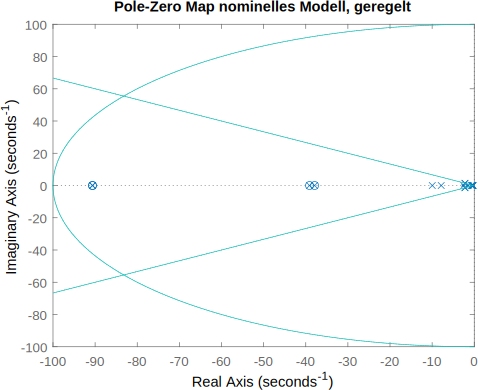
\includegraphics[width=\linewidth]{./Bilder/pzmap_controlled.eps}
		\caption{Vollständiges Polgebiet}
		\label{fig:pzmap_controlled_ohnezoom}
	\end{subfigure}
	\hfill
	\begin{subfigure}{.49\textwidth}
		\centering
		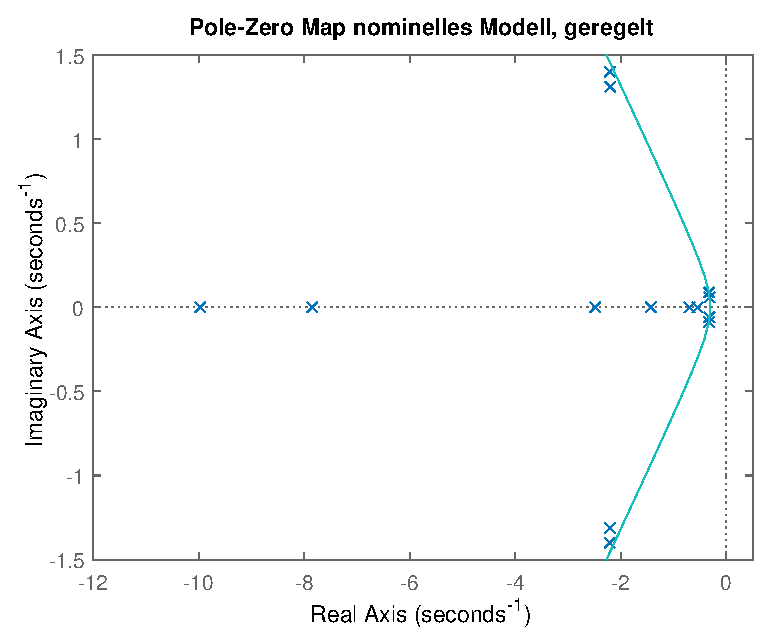
\includegraphics[width=\linewidth]{./Bilder/pzmap_controlled_zoom.eps}
		\caption{Polgebiet mit Fokus auf den Ursprung}
		\label{fig:pzmap_controlled_zoom}
	\end{subfigure}
	\caption{Pol-/ Nullstellendiagramm des geregelten linearen Systems}
	\label{fig:pzmap_controlled}
\end{figure}

In den Abbildungen \ref{fig:outputs_linear_ohne_stellbesch} und \ref{fig:stellgr_linear_ohne_stellbesch} sind die Sprungantworten sowie die Stellgrößenverläufe des linearen Modells ohne Einfluss der Stellgrößenbeschränkungen für Änderungen um den Arbeitspunkt dargestellt. 
\begin{figure}[H] % figure outputs nur linear ohne stellgrößenbeschränkung
	\centering
	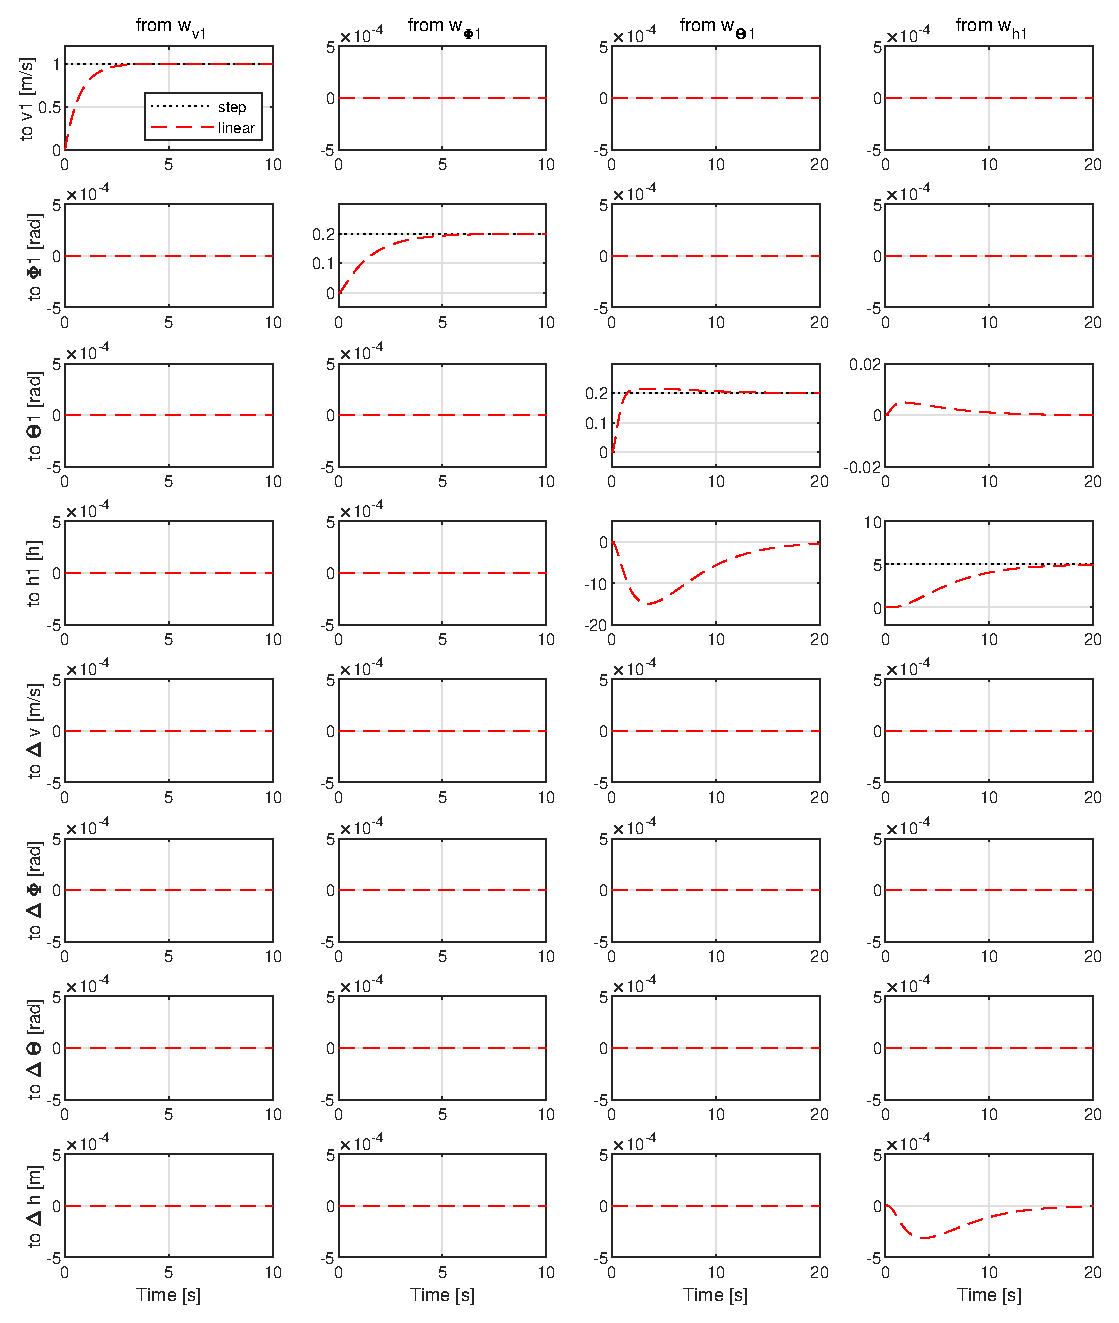
\includegraphics[width=\linewidth]{./Bilder/outputs_lin_ohne_beschr_um_AP.eps}
	\caption{Sprungantworten \textbf{ohne} Wirkung der Stellgrößenbeschränkung bei sprungförmigen Änderungen um den Arbeitspunkt, lineares System}
	\label{fig:outputs_linear_ohne_stellbesch}
\end{figure}
Für die Führungsgrößen $v_1$ und $h_1$ werden Sprünge von $\valunit{1}{m/s}$ respektive $\valunit{5}{m}$ ausgehend vom eigentlichen Arbeitspunkt vorgegeben. Für die beiden Eulerwinkel $\Phi_1$ und $\Theta_1$ werden Sprünge von jeweils $\valunit{0.2}{rad}$ gewählt, was $\valunit{11.46}{\degree}$ entspricht. Bei Betrachtung der Sprungantworten in Abbildung \ref{fig:outputs_linear_ohne_stellbesch} ist gut zu erkennen, dass die Verkopplung für alle Größen erfolgreich ist. Lediglich Führungssprünge auf $h_1$ führen dazu, dass $\Delta h$ minimal schwingt, was nach etwa \valunit{15}{s} allerdings wieder abgeklungen ist. Es ist außerdem zu erkennen, dass $v_1$ seinen Endwert nach \valunit{2}{s} ohne Überschwingen und entkoppelt von den anderen Ausgängen des ersten Flugzeugs stationär genau erreicht. Das gleiche gilt für $\Phi_1$ nach \valunit{5}{s}. Bei Betrachtung der Sprungantworten von $\Theta_1$ und $h_1$ fällt zudem auf, dass sich diese Größen gegenseitig beeinflussen, was durch die Wahl der Übertragungsmatrix zulässig ist. Die anderen Ausgangsgrößen von Flugzeug 1 werden dabei nicht beeinflusst. Diese beiden Größen benötigen jeweils etwa \valunit{15}{s} bis zum Erreichen des stationären Endwerts. Ein Sprung auf $\Theta_1$ führt dabei zu einem Höhenverlust von \valunit{15}{m} bevor die Höhe wieder auf ihren Sollwert zurückgestellt wird, während ein Höhensprung lediglich einen sehr geringen Einfluss auf $\Theta_1$ hat. 
\begin{figure}[H] % figure nur linear stellgrößen
	\centering
	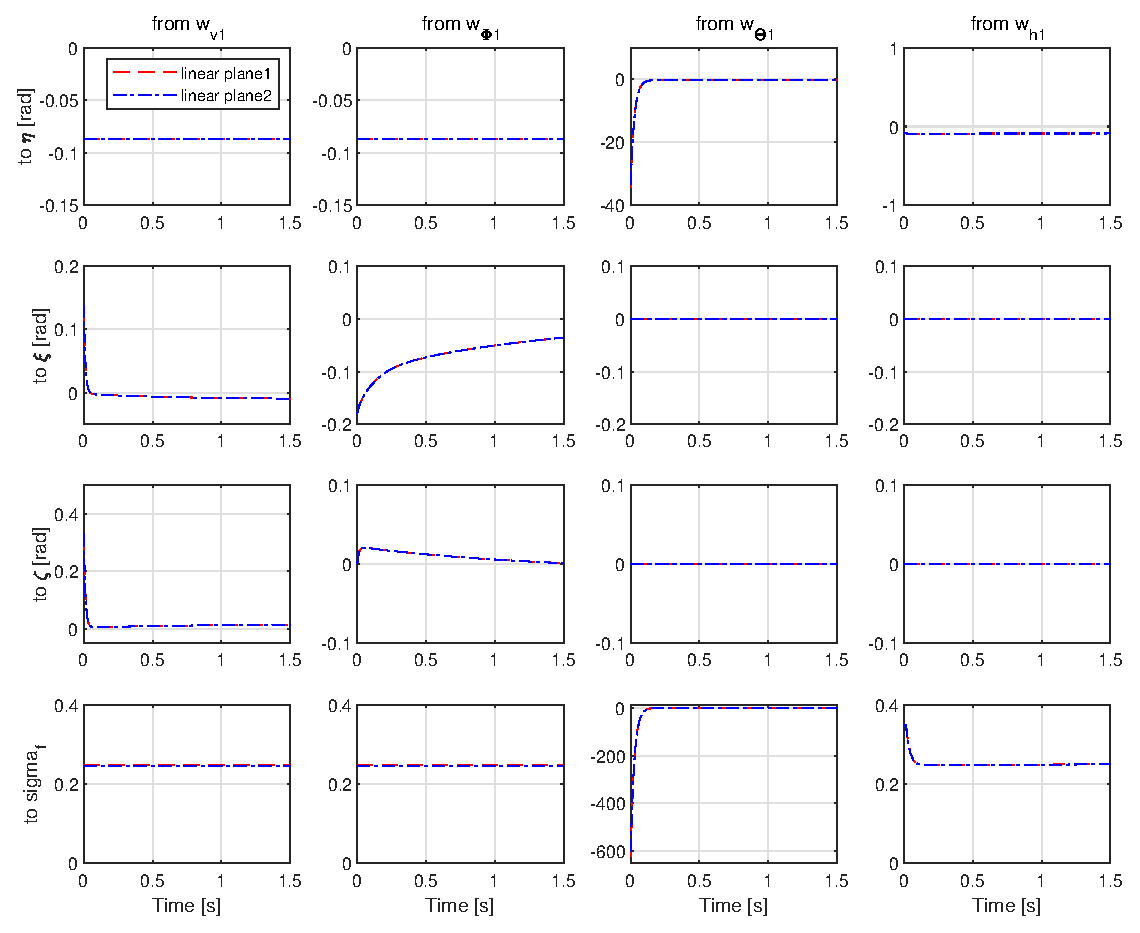
\includegraphics[width=\linewidth]{./Bilder/stellgr_linear_ohne_stellbeschr.eps}
	\caption{Stellgrößen \textbf{ohne} Wirkung der Stellgrößenbeschränkung bei sprungförmigen Änderungen um den Arbeitspunkt, lineares System}
	\label{fig:stellgr_linear_ohne_stellbesch}
\end{figure}
Bei Betrachtung der Stellgrößenverläufe in Abbildung \ref{fig:stellgr_linear_ohne_stellbesch} fällt zunächst auf, dass diese für die beiden Flugzeuge nahezu identisch sind. Zudem lässt sich feststellen, dass beim Aufschalten von Führungssprüngen - mit Ausnahme von $\Theta_1$ - die Stellgrößenbeschränkungen nicht verletzt werden. Bei $\Theta_1$ hingegen führt schon ein relativ geringer Sprung zu sehr hohen Stellgrößen, die jenseits der Grenzwerte für die Stellgrößen liegen. Bei Einführung der Stellgrößenbeschränkungen wird diese Eigenschaft zu unerwünschtem bis hin zu instabilem Systemverhalten führen. 

\section{Vergleich des linearen Modells mit dem nichtlinearen Modell unter Verwendung der Stellgrößenbeschränkungen}
Im Folgenden wird ebendieser Fall verdeutlicht. Die Abbildungen \ref{fig:stellgr_linear_nlinear_mit_stellbeschr} und \ref{fig:outputs_linear_nlinear_mit_stellbeschr} zeigen das Verhalten des linearen Modells im Vergleich mit dem nichtlinearen Modell unter Einfluss der Stellgrößenbeschränkung für sprungförmige Änderungen um den Arbeitspunkt. 
\begin{figure}[H] % figure stellgrößen linear und nlinear mit stellgrößenbeschränkung
	\centering
	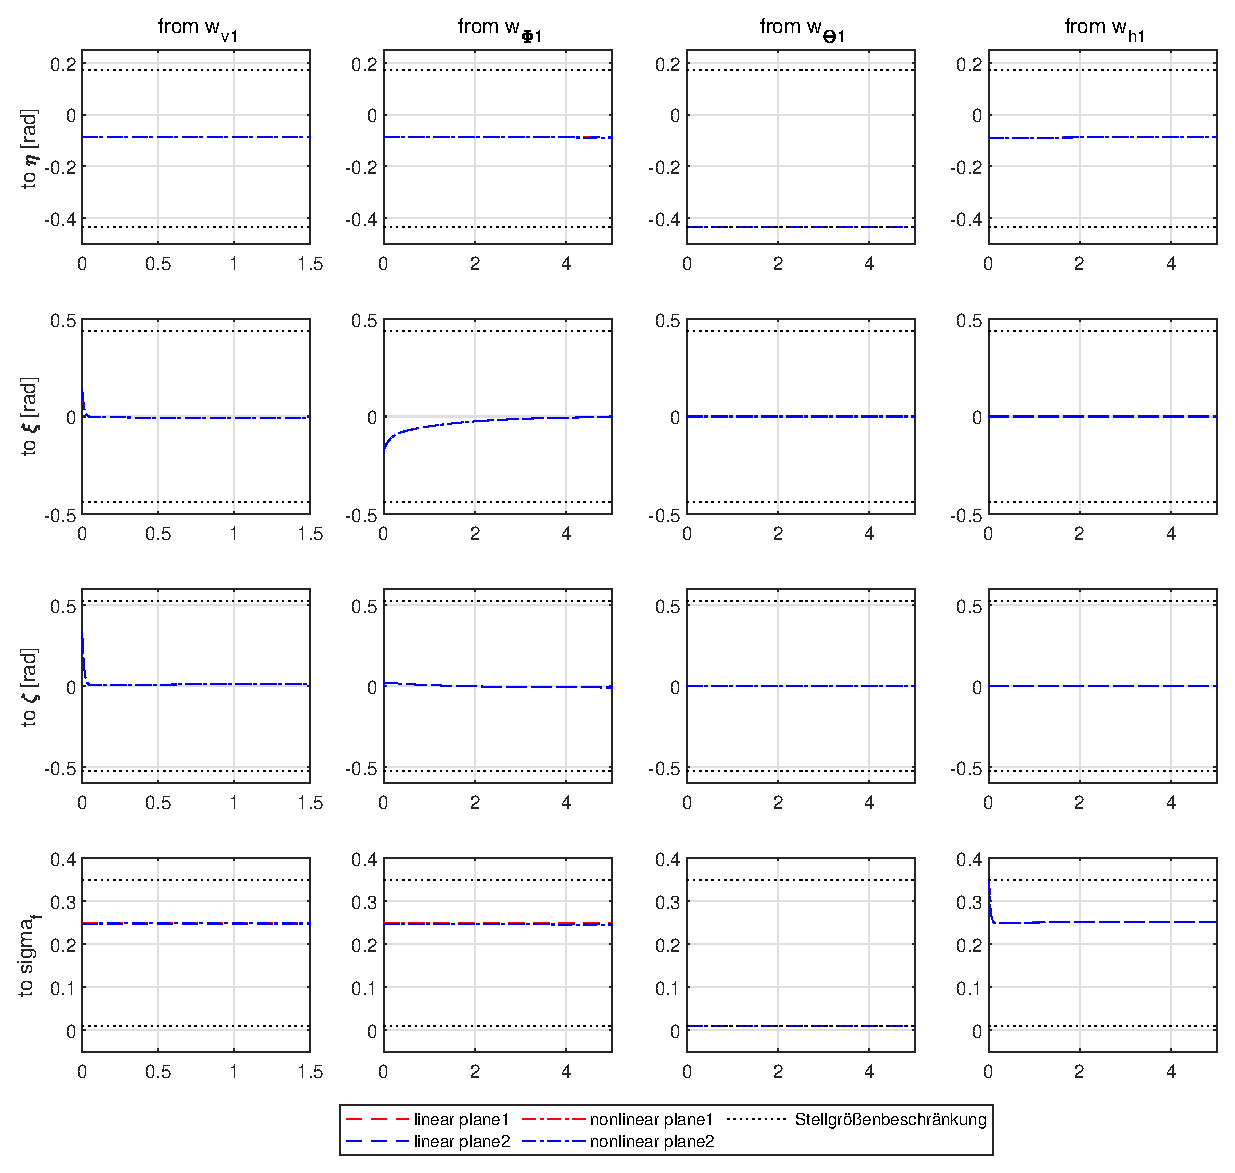
\includegraphics[scale=0.75]{./Bilder/stellgr_linear_nlinear_mit_stellbeschr_plot_stellgr.eps}
	\caption{Stellgrößen des linearen und nichtlinearen Modells \textbf{mit} Wirkung der Stellgrößenbeschränkung bei sprungförmigen Änderungen um den Arbeitspunkt}
	\label{fig:stellgr_linear_nlinear_mit_stellbeschr}
\end{figure}
Die gepunkteten Linien stellen die jeweiligen Stellgrößenbeschränkungen dar. Bei Betrachtung der dritten Spalte von Abbildung \ref{fig:stellgr_linear_nlinear_mit_stellbeschr} fällt zunächst auf, dass die Stellgrößen $\eta$ und $\tn{sigma}_f$ bei Anregung von $\Theta_1$ durch die unteren Grenzwerte der Stellgrößen begrenzt werden. Wie in Abbildung \ref{fig:outputs_linear_nlinear_mit_stellbeschr} zu erkennen ist, führt dies zu unerwünschtem Systemverhalten (Änderung von $\Phi_1$ um mehr als \valunit{110}{\degree}), was darauf zurückzuführen ist, dass die Stellgrößenbeschränkung in diesem Fall wie eine Öffnung der Regelschleife wirkt. Es kann auf Zustandsänderungen nicht mehr sinngemäß reagiert werden, wodurch sich das System schnell vom Arbeitspunkt entfernt. Das Modell verliert damit für diesen Bereich seine Gültigkeit. Dieser Einfluss wirkt sich beim linearen Modell allerdings stärker aus als beim nichtlinearen Modell. Dies zeigt sich darin, dass die Verkopplung beim nichtlinearen Modell, insbesondere bei der Höhe, besser erreicht wird.
\begin{figure}[H] % figure outputs linear und nlinear mit stellgrößenbeschränkung
	\centering
	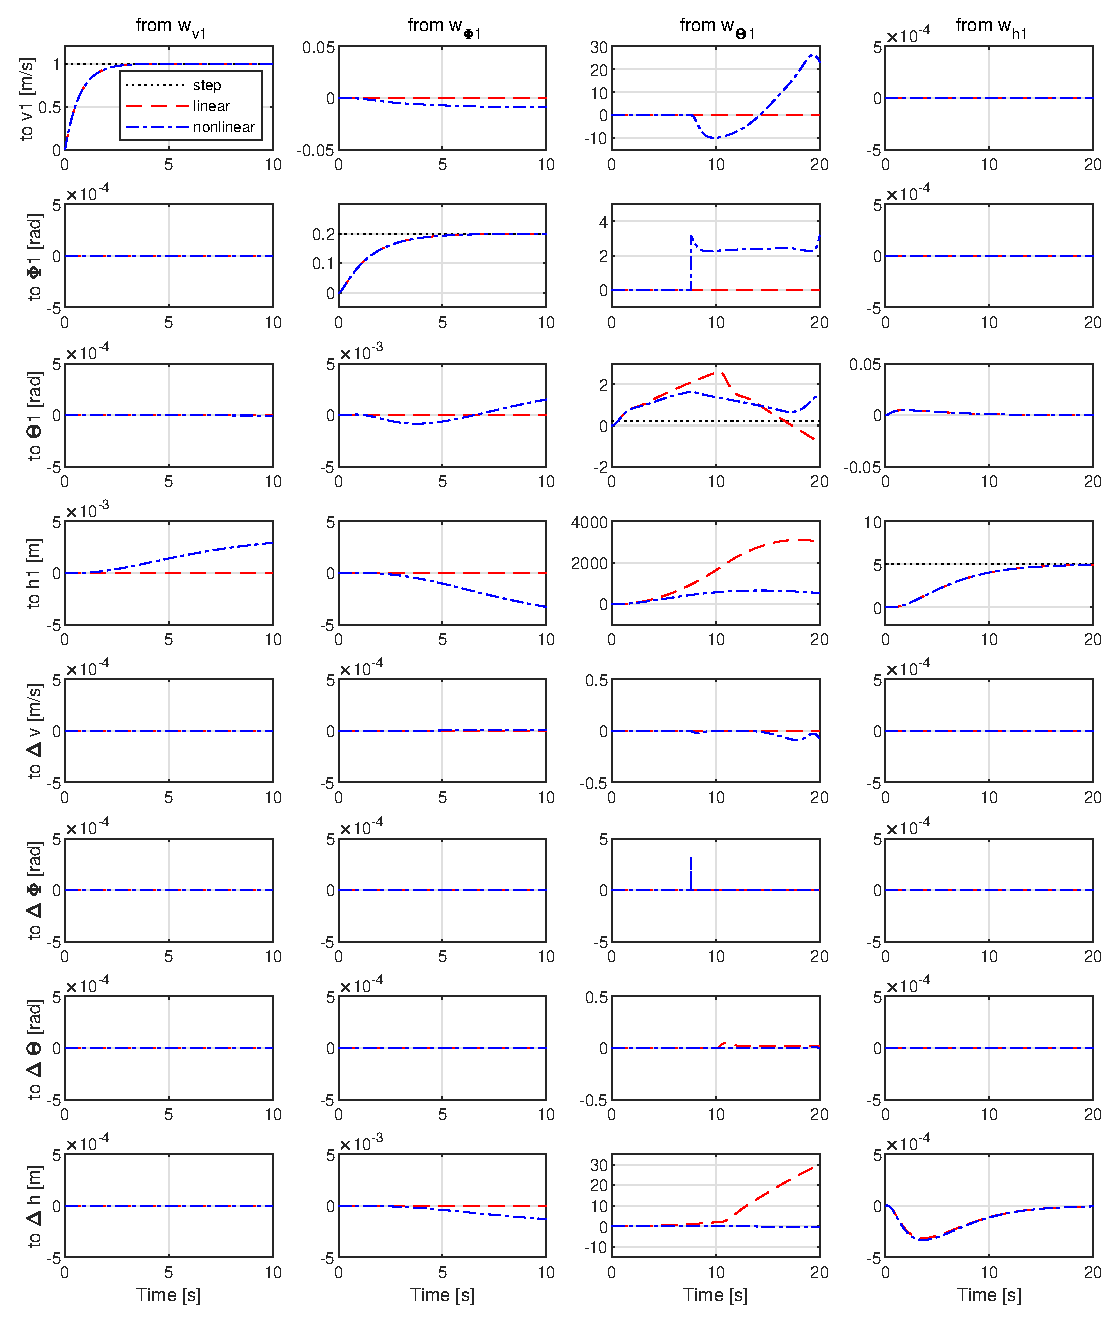
\includegraphics[width=\linewidth]{./Bilder/outputs_lin_nlin_mit_beschr_um_AP.eps}
	\caption{Sprungantworten des linearen und nichtlinearen Modells \textbf{mit} Wirkung der Stellgrößenbeschränkung bei sprungförmigen Änderungen um den Arbeitspunkt}
	\label{fig:outputs_linear_nlinear_mit_stellbeschr}
\end{figure}
Des Weiteren fällt auf, dass bei den Anregungen von $v_1, \Phi_1$ und $h_1$ die Verkopplung sowohl für das lineare als auch für das nichtlineare Modell erreicht wird. Außerdem lässt sich feststellen, dass die beiden Modelle am Arbeitspunkt zwar relativ gut miteinander übereinstimmen, es aber teilweise leichte Abweichungen gibt. Diese Unterschiede sind unter anderem in der Übertragungsfunktion $\Phi_1 \rightarrow h_1$ zu erkennen und führen dazu, dass die Entkopplung der einzelnen Ein- und Ausgänge von Flugzeug 1 beim nichtlinearen Modell teilweise nicht erreicht wird. Sie sind darauf zurückzuführen, dass das lineare Modell das Systemverhalten des nichtlinearen Modells bei Abweichungen vom Arbeitspunkt nicht mehr exakt widerspiegelt. Das lineare Modell ist nur genau im Arbeitspunkt exakt. Zudem zeigt Abbildung \ref{fig:stellgr_linear_nlinear_mit_stellbeschr}, dass bei den entsprechenden Sprunghöhen für $v_1, \Phi_1$ und $h_1$ die Stellgrößenbeschränkungen weder beim linearen noch beim nichtlinearen Modell verletzt werden. 

\subsection{Verkopplung der Flugzeugpositionen}
Eine weitere Anforderung an die Regelung ist die Verkopplung der Flugzeugpositionen. Diese wird im Folgenden betrachtet und analysiert. Der Abstand der Flugzeuge bezüglich des erdfesten Referenzkoordinatensystems ist in Abbildung \ref{fig:distance_xyz_nlinear} für das nichtlineare Modell dargestellt. Es ist gut zu erkennen, dass bei allen Sprunganregungen mit Ausnahme von $\Theta_1$ die Verkopplung der Flugzeugpositionen über den Simulationszeitraum gegeben ist. Der Abstand in Richtung der $y-$Achse beträgt null Meter. Für die $x-$Achse und die $z-$Achse beträgt der Abstand jeweils \valunit{10}{m}, was den gewünschten Werten im Arbeitspunkt entspricht. Die Darstellung über den relativ kurzen Zeitraum soll jedoch keine Einschränkung sein, da die Zustände nach Ablauf der Simulation bereits im eingeschwungenen Zustand sind. Das heißt, auch über einen längeren Zeitraum oder bei mehrfacher Anregung wäre die Verkopplung gewährleistet. Eine Anregung von $\Theta_1$ führt allerdings zu einer Abweichung der Werte von ihren Sollwerten und damit zu einem Verlust der Verkopplung der Positionen. 
\begin{figure}[h] % figure distanz zwischen flugzeugen
	\centering
	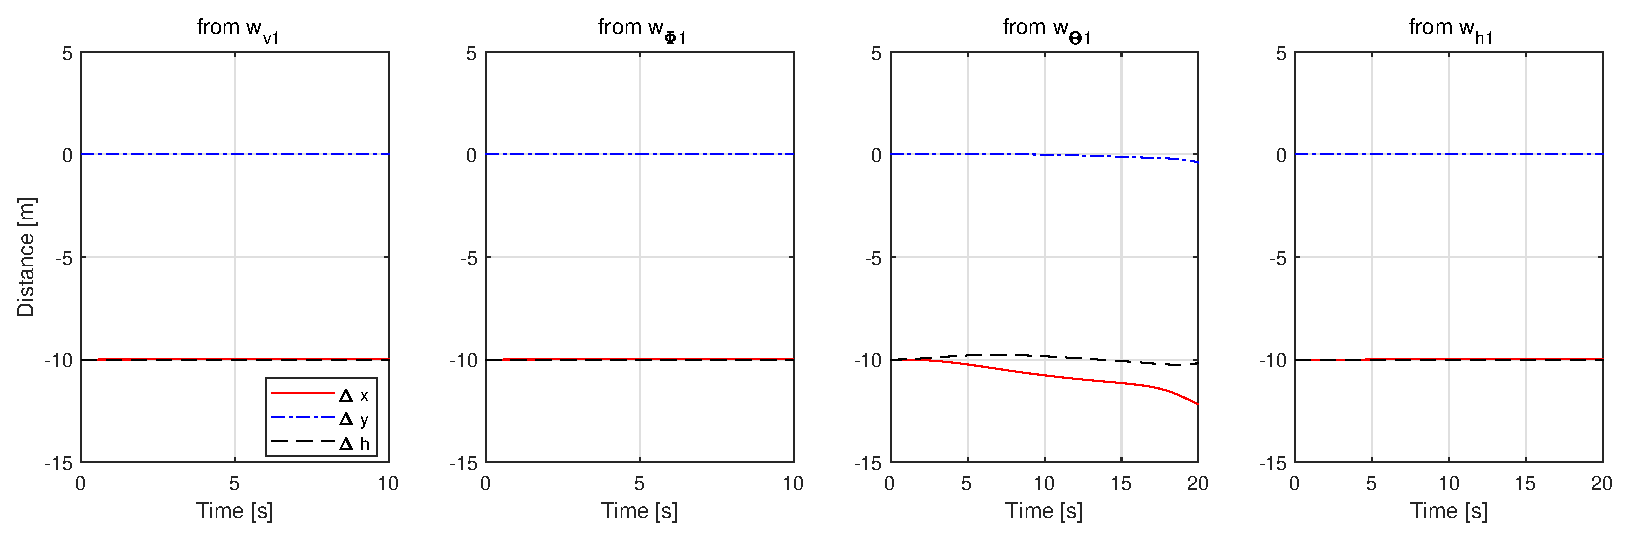
\includegraphics[scale=0.6]{./Bilder/distance_xyz_nlinear.eps}
	\caption{Abstand der Flugzeuge bezüglich des erdfesten Referenzsystems für das nichtlinearen Modell}
	\label{fig:distance_xyz_nlinear}
\end{figure}
Als Zwischenfazit lässt sich also festhalten, dass die Regelung prinzipiell dazu in der Lage ist, die Flugzeuge miteinander zu verkoppeln und auch die Entkopplung der Führungsgrößen von Flugzeug 1 wie gewünscht erreicht wird. Führungssprünge des Nickwinkels führen allerdings zu enorm hohen Stellgrößen, welche durch die Stellgrößenbeschränkung begrenzt werden und dadurch zum Verlust der gewünschten Eigenschaften führen. Die Regelung reagiert sehr sensitiv auf derartige Änderungen.

\section{Ergebnisse Parameterschwankungen der Flugzeugmasse}\label{sec:Parameterschwankungen}
Nachdem nun das Systemverhalten des linearen und des nichtlinearen Modells für das nominelle Modell miteinander verglichen und hinsichtlich der Anforderungen an die Regelung diskutiert wurde, soll nun der Einfluss von Parameterschwankungen in Form von unterschiedlichen Flugzeugmassen am nichtlinearen Modell analysiert werden. 
\subsection{Einführung der Modelle unter Parameterschwankung}
Die Parameterschwankung wirkt dabei so, dass zu Beginn der Betankung Flugzeug 1 (Tankflugzeug) zusätzliche zu seiner eigenen Masse die Masse des Treibstoffs transportiert, während Flugzeug 2 (betanktes Flugzeug) nur seine eigene Masse transportiert (siehe Kapitel \ref{cha:ZweiFlieger}). Es gilt also 
\begin{align}
	m_1 = m + \sigma m_\tn{ks}, \qquad m_2 = m, \qquad \tn{mit} \, \sigma\in\lbrack0,1\rbrack,
\label{eq:massmodel1}
\end{align}
wobei die Parameterschwankung über den Parameter $\sigma$ zwischen 0 und \valunit{100}{\%} der gesamten Treibstoffmasse variiert werden kann. Dieser Fall wird nachfolgend als Modell 2 bezeichnet.
Nach Abschluss der Betankung hat das Tankflugzeug die Treibstoffmasse an das zu betankende Flugzeug abgegeben und es gilt entsprechend
\begin{align}
	m_1 = m , \qquad m_2 = m + \sigma m_\tn{ks}, \qquad \tn{mit} \, \sigma\in\lbrack0,1\rbrack.
\label{eq:massmodel2}
\end{align}
Dieser Fall wird nachfolgend als Modell 3 bezeichnet.

\subsection{Reglerauslegung mittels Multi-Modell-Ansatz}
Um einen bezüglich der Massenschwankung möglichst robusten Regler entwerfen, wird mit \texttt{gammasyn} versucht ein Regler mittels Multi-Modell-Ansatz auszulegen (siehe Kapitel \ref{cha:GrundlagenReg}). Dazu wird die Parameterschwankung zunächst sehr gering gewählt, damit die betrachteten Modelle nicht zu stark vom nominellen Modell abweichen. Die Treibstoffmasse wird mit $\sigma=0.1$ zu \valunit{1400}{kg} gewählt. Damit beträgt die Abweichung bezogen auf das nominelle Gewicht \valunit{1.167}{\%}. Es konnte festgestellt werden, dass unter Verwendung des in Kapitel \ref{cha:Regler} erklärten Polgebiets zur Einhaltung der Mindestanforderngen keine Lösung für das Optimierungsproblem gefunden werden kann. Daher werden die Anforderungen bezüglich des Polgebiets auf das Mindeste, die Forderung nach Stabilität, beschränkt und es wird als zulässiges Polgebiet der gesamte Bereich links der Imaginärachse gewählt. 

Abbildung \ref{fig:pzmap_multi_modell_ansatz} zeigt die Lage der Pol- und Nullstellen für die drei Modelle. Wie gut zu erkennen ist, können für keines der beiden Polgebiete alle Eigenwerte innerhalb des Polgebiets platziert werden. Es ist selbst bei der geringen Schwankung der Masse nicht möglich alle Eigenwerte links der Imaginärachse zu platzieren, was zu instabilem Verhalten führt. Es lässt sich schlussfolgern, dass kein robuster Verkopplungsregler für Schwankungen der Masse ausgelegt werden kann, der alle Systeme zumindest stabilisiert. 
\begin{figure}[h] % figure pzmap multimodell ansatz
	\centering
	\begin{subfigure}{.49\textwidth}
		\centering
		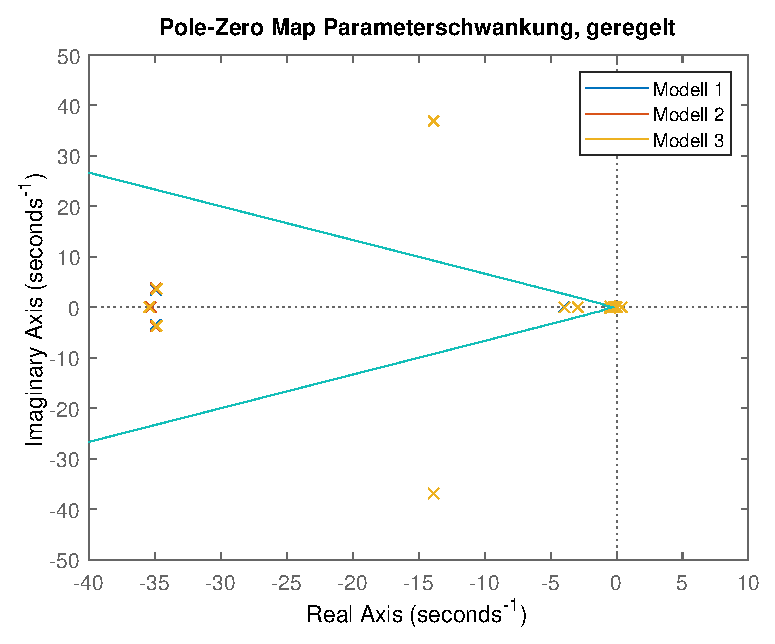
\includegraphics[width=\linewidth]{./Bilder/pzmap_multi_modell_10prozent_hyperbola.eps}
		\caption{Multi-Modell-Ansatz für das Polgebiet aus Kapitel \ref{cha:Regler}}
		\label{fig:pzmap_multi_modell_10prozent_hyperbola}
	\end{subfigure}
	\hfill
	\begin{subfigure}{.49\textwidth}
		\centering
		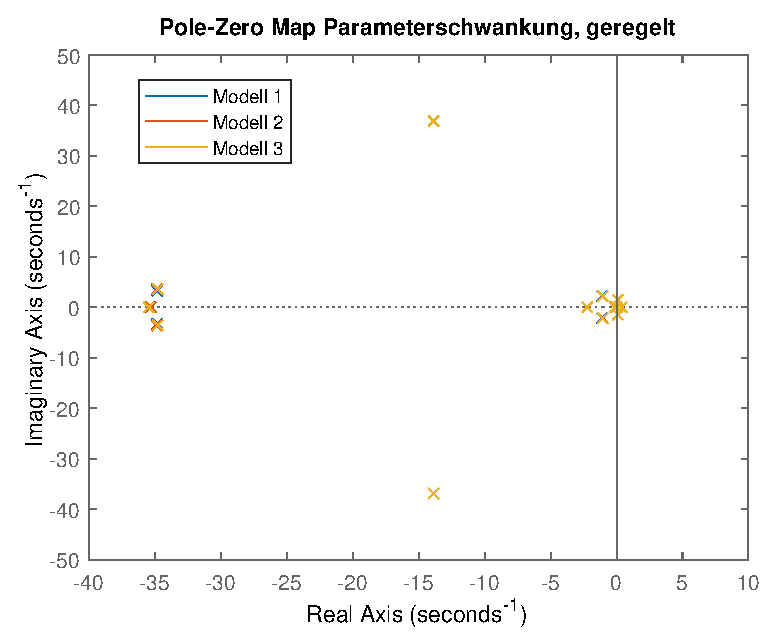
\includegraphics[width=\linewidth]{./Bilder/pzmap_multi_modell_10prozent_imag.eps}
		\caption{Multi-Modell-Ansatz für das Polgebiet links der Imaginärachse}
		\label{fig:pzmap_multi_modell_10prozent_imag}
	\end{subfigure}
	\caption{Pol-/ Nullstellendiagramm der drei Systeme unter Einfluss von Parameterschwankungen für das nominelle System (Modell 1), das System vor dem Betankungsvorgang (Modell 2) und das System nach Abschluss der Betankung (Modell 3) jeweils mit $\sigma=0.1$. Für jedes Polgebiet wird ein Regler mittels Multi-Modell-Ansatz ausgelegt.}
	\label{fig:pzmap_multi_modell_ansatz}
\end{figure}

\subsection{Reglerperformance von $\mat{K}_\tn{koppel}$ bezüglich der Modelle 2 und 3}
Nachdem zuvor gezeigt wurde, dass das System höchst sensitiv auf Schwankungen der Flugzeugmasse reagiert und mittels Multi-Modell-Ansatz nicht einmal Stabilität für alle drei Modelle gewährleistet werden kann, soll nachfolgend die Performance des in Kapitel \ref{cha:Regler} ausgelegten Verkopplungsreglers $\mat{K}_\tn{koppel}$ für die Modelle 2 und 3 evaluiert werden. Durch die unterschiedlichen Massen ergeben sich leicht abweichende Arbeitspunkte und dadurch auch unterschiedliche Systemmatrizen. Bei Vorgabe der entsprechenden Größen zur Bestimmung des Arbeitspunktes für den Geradeausflug (siehe Kapitel \ref{cha:Linearisierung}) ändern sich durch die zusätzliche Masse die Größen $w, \Theta, \eta$ und $\tn{sigma}_f$. Bei voller Treibstoffmasse ($\sigma=1$) gilt im Arbeitspunkt
\begin{align*}
w_\tn{AP1} = \valunit{-9.3012}{m/s}, \quad \Theta_\tn{AP1} = \valunit{-0.0619}{rad}, \quad \eta_\tn{AP1} = \valunit{-0.0954}{rad}, \quad \tn{sigma}_{f\tn{AP1}} = 0.2254
\end{align*}
für das auf \valunit{5000}{m} fliegende Flugzeug 1 und 
\begin{align*}
w_\tn{AP2} = \valunit{-9.2834}{m/s}, \quad \Theta_\tn{AP2} = \valunit{-0.0618}{rad}, \quad \eta_\tn{AP2} = \valunit{-0.0955}{rad}, \quad \tn{sigma}_{f\tn{AP2}} = 0.2252
\end{align*}
für das auf \valunit{5010}{m} fliegende Flugzeug 2. Abbildung \ref{fig:pzmap_controlled_schwankung} zeigt das Pol-/ Nullstellendiagramm für das nominelle Modell, Modell 2 und Modell 3. Wie aus der Abbildung zu erkennen ist, können bei der Regelung mit $\mat{K}_\tn{koppel}$ auch für die Modelle 2 und 3 die invarianten Nullstellen durch Eigenwerte kompensiert und alle Eigenwerte innerhalb des vorgegebenen Polgebiets platziert werden.
\begin{figure}[h] % figure pzmap multimodell
	\centering
	\begin{subfigure}{.49\textwidth}
		\centering
		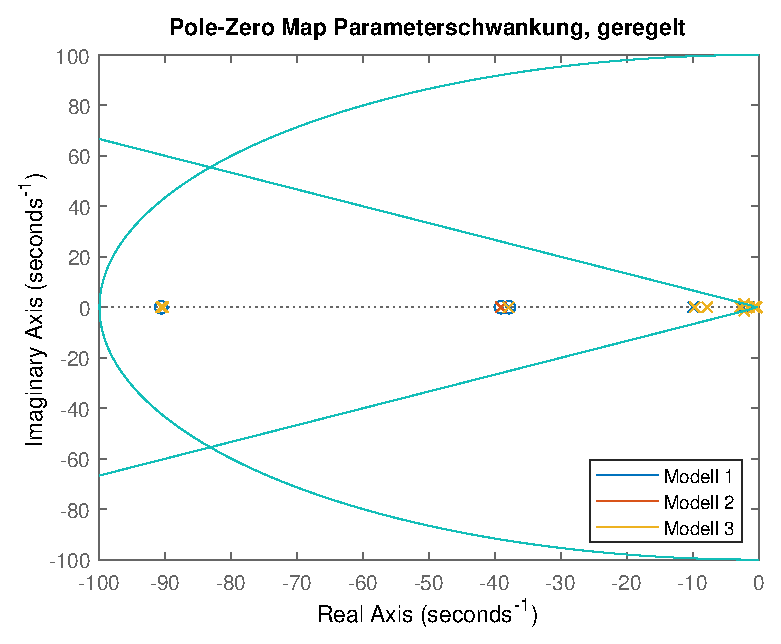
\includegraphics[width=\linewidth]{./Bilder/pzmap_controlled_schwankung.eps}
		\caption{Vollständiges Polgebiet}
		\label{fig:pzmap_controlled_schwankung_ohne_zoom}
	\end{subfigure}
	\hfill
	\begin{subfigure}{.49\textwidth}
		\centering
		\includegraphics[width=\linewidth]{./Bilder/pzmap_controlled_schwankung_zoom.eps}
		\caption{Polgebiet mit Fokus auf den Ursprung}
		\label{fig:pzmap_controlled_schwankung_zoom}
	\end{subfigure}
	\caption{Pol-/ Nullstellendiagramm der drei durch $\mat{K}_\tn{koppel}$ geregelten Modelle mit $\sigma=1$ (volle Tankladung).}
	\label{fig:pzmap_controlled_schwankung}
\end{figure}

Die Sprungantworten zu den Modellen 2 und 3 sowohl für den linearen als auch den nichtlinearen Fall sind in Abbildung \ref{fig:outputs_linear_nlinear_two_masses} dargestellt.
Wie bereits beim nominellen Modell, führen auch bei den Modellen 2 und 3 Führungssprünge auf $\Theta_1$ zu instabilem Verhalten. Da die starke Sensitivität des Systems bezüglich Änderungen von $\Theta_1$ bereits umfassend erläutert wurde, soll an dieser Stelle nicht weiter darauf eingegangen werden. Stationäre Genauigkeit ist bei Sprüngen auf $v_1$ und $\Phi_1$ bezüglich der jeweiligen Führungsgrößen nach wie vor gewährleistet. Es fällt allerdings auf, dass die Parameterschwankung der Masse Einfluss auf das Gesamtverhalten hat. So ist der Einfluss von $\Phi_1$ auf $v_1$ nun etwas stärker. Während die zusätzliche Masse beim linearen Modell keinen Einfluss auf die Höhe hat und sowohl die Sollhöhe $h_1$ gehalten wird als auch die Verkopplung der Höhe uneingeschränkt funktioniert, gilt dies für das nichtlineare Modell nicht. Es lässt sich erkennen, dass bei Sprüngen auf $v_1$ und $\Phi_1$ die Sollhöhe beim nichtlinearen Modell nicht gehalten werden kann und die zusätzliche Masse zu einem stationären Höhenverlust führt. Dadurch ist auch die Verkopplung der Höhen nicht mehr gewährleistet. Im Fall, dass Flugzeug 1 das schwerere Flugzeug ist (Modell 2), verliert es an Höhe, ohne dass Flugzeug 2 folgt, sodass der Abstand zwischen den beiden Flugzeugen größer wird. Im Fall, dass Flugzeug 2 bereits betankt wurde (Modell 3), ist es genau umgekehrt - die Flugzeuge nähern sich einander an. Dies gilt sowohl für Führungsgrößensprünge auf $v_1$ als auch auf $\Phi_1$. Außerdem entsteht im nichtlinearen Modell bei Sprüngen auf $v_1$ eine bleibende Abweichung für $\Delta v$ sowie $\Delta \Phi$. 

Führungssprünge bezüglich der Höhe haben keinerlei Einfluss auf $v_1$ und $\Phi_1$ und auch $\Theta_1$ wird nur leicht um den Arbeitspunkt herum ausgelenkt. Allerdings führt die Treibstoffmasse dazu, dass die stationäre Genauigkeit bezüglich der Höhe im nichtlinearen Modell verloren geht, sofern Flugzeug 1 das schwerere ist, da der Regler nicht dazu in der Lage ist diese Schwankung auszuregeln. Dies schlägt sich ebenfalls im verkoppelten Ausgang $\Delta h $ nieder. Ist Flugzeug 2 das schwerere, so wird der Sollwert bezüglich $h_1$ zwar stationär genau erreicht, jedoch gelingt es nicht, das schwerere Flugzeug 2 nachzuführen, sodass auch in diesem Fall eine bleibende Höhendifferenz entsteht. 
\begin{figure}[H] % figure sprungantworten zwei massenmodelle
	\centering
	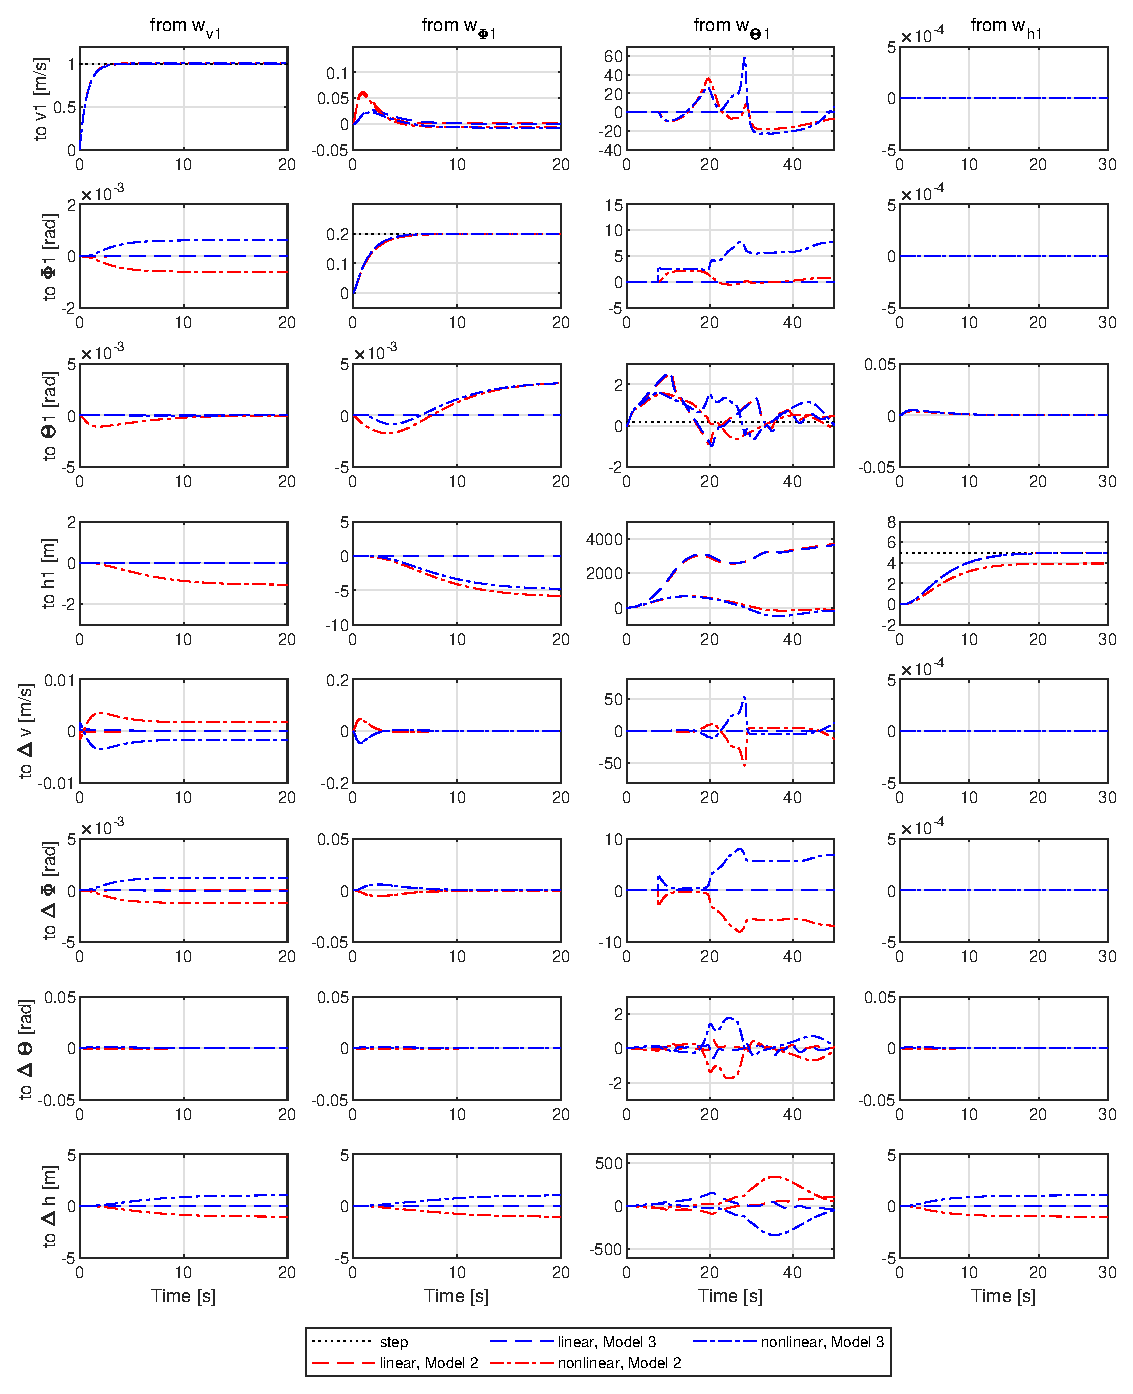
\includegraphics[width=\linewidth]{./Bilder/outputs_lin_nlin_two_masses_um_AP.eps}
	\caption{Sprungantworten der mit $\mat{K}_\tn{koppel}$ geregelten Modelle 2 und 3 für das lineare und nichtlineare Modell bei sprungförmigen Änderungen um den Arbeitspunkt}
	\label{fig:outputs_linear_nlinear_two_masses}
\end{figure}
Abbildung \ref{fig:distance_xyz_nlinear_twomassmodels} zeigt die Positionsdifferenz der beiden Flugzeuge für die Modelle 2 und 3. Es ist deutlich zu erkennen, dass die Regelung bei keinem der Modelle dazu in der Lage ist, die Positionen miteinander zu verkoppeln. Dies liegt daran, dass die Parameterschwankung zu einer Abweichung des Modells vom nominellen Modell führt, für das die Regelung ausgelegt wurde. Da die Positionen nicht Bestandteil der in der Zustandsrückführung geregelten Zustände sind, hat die Regelung keine Möglichkeit auf Positionsdifferenzen zu reagieren. Abweichungen in der Geschwindigkeit und den Kurswinkeln $\gamma$ und $\chi$ werden aufintegriert, ohne darauf Einfluss nehmen zu können. 
\begin{figure}[H] % figure positionsdifferenz zwei massenmodelle
	\centering
	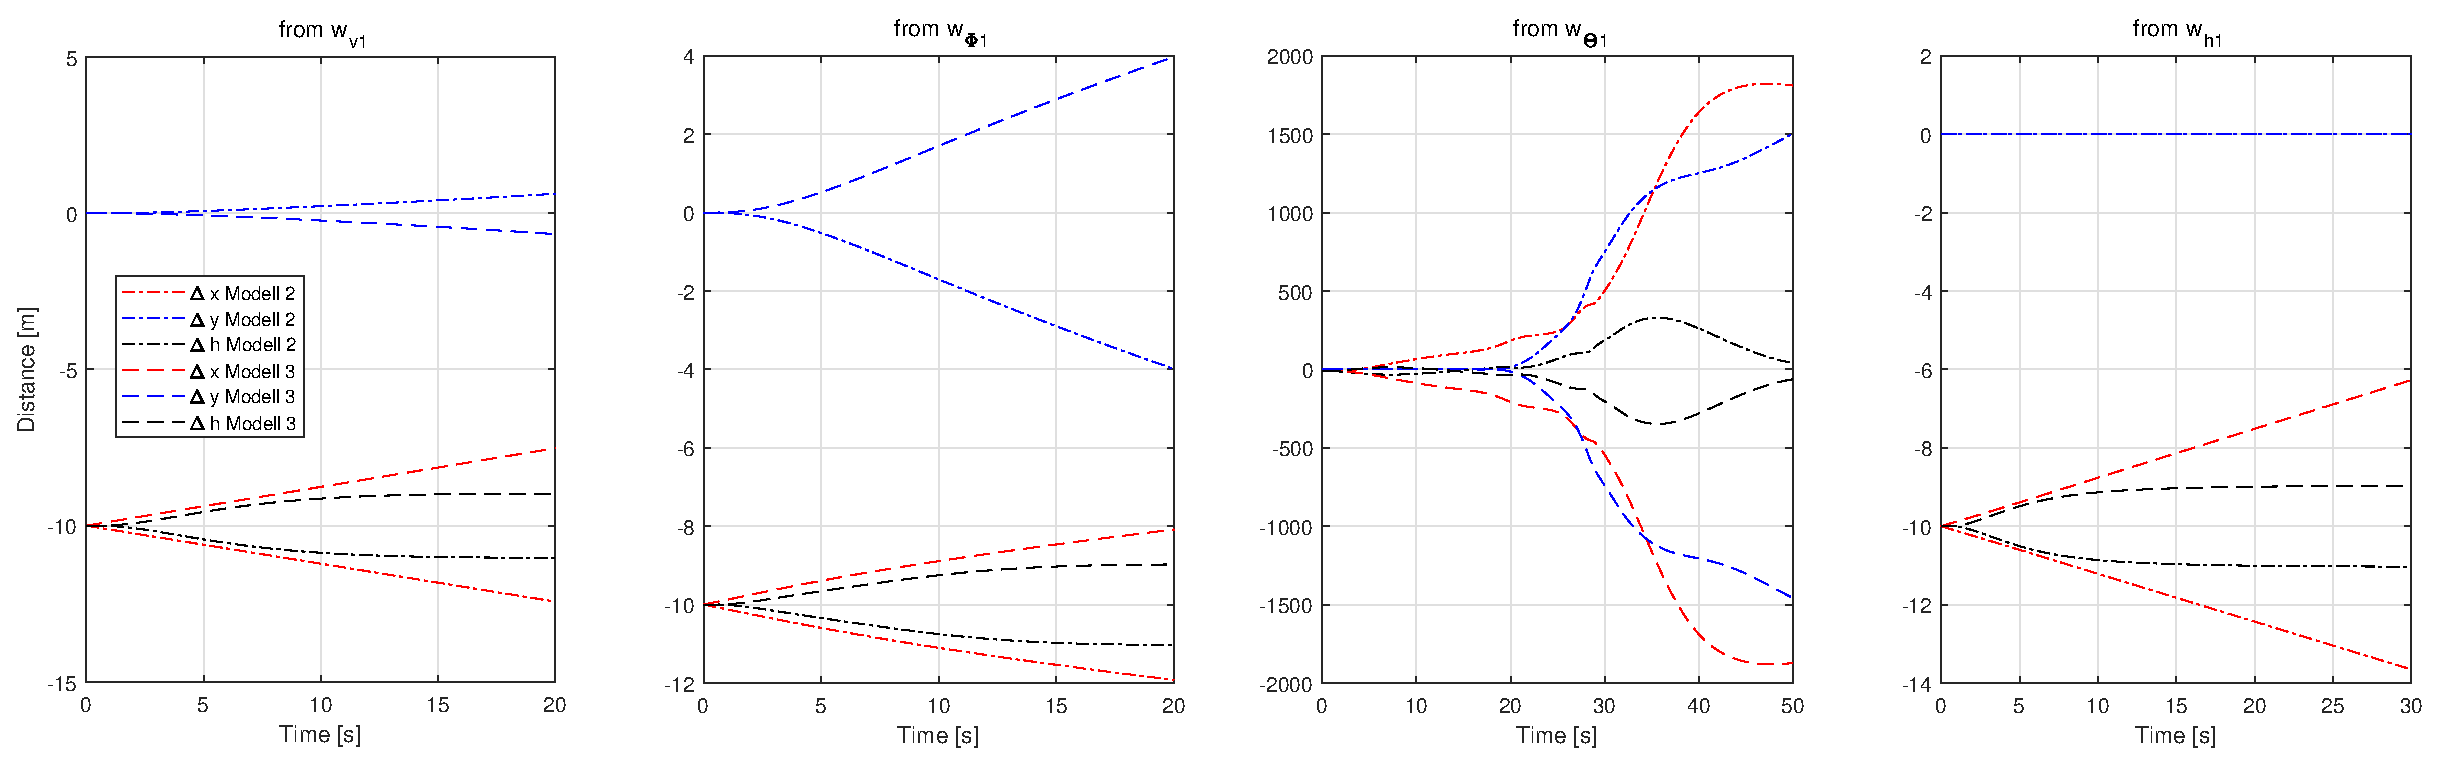
\includegraphics[width=\linewidth]{./Bilder/distance_xyz_nlinear_twomassmodels.eps}
	\caption{Abstand der Flugzeuge für die durch die durch die Massenschwankung beeinflussten nichtlinearen Modelle 2 und 3, geregelt mit $\mat{K}_\tn{koppel}$}
	\label{fig:distance_xyz_nlinear_twomassmodels}
\end{figure}
Damit lässt sich als Abschluss dieses Abschnitts festhalten, dass die Verkopplungsregelung den Einfluss der Parameterschwankung in der Flugzeugmasse nicht ausregeln kann. Bei Abweichung vom für die Reglerauslegung gültigen Modell, ist die Verkopplung der Flugzeuge nicht mehr gewährleistet. Geringere Schwankungen in der Masse führen zwar dazu, dass sich das System langsamer vom Arbeitspunkt entfernt und der Verlust der Verkopplung langsamer geschieht, das prinzipielle Systemverhalten ist allerdings gleich. Die Robustheit gegenüber derartigen Schwankungen ist nicht gegeben. 

\section{Strukturelle Erweiterung für das nominelles Modell}
Neben Parameterschwankungen können auch andere Störfaktoren das Systemverhalten beeinflussen. Äußere Störeinflüsse, die zum Beispiel in Form von Wind oder Luftlöchern in das System eingreifen, können dazu beitragen, dass das Systemverhalten instabil wird. Daher sollten diese durch die Regelung ausgeregelt werden. Die Störungen werden als sprungförmige Störgrößen, die auf die Zustände wirken, modelliert. Um derartige Störungen stationär genau ausregeln zu können, muss der Regelkreis vor dem Einfluss der Störgröße einen I-Anteil besitzen. Da dies durch den Verkopplungsregler nicht gewährleistet ist, wird im Folgenden zusätzlich zum Zustandsregler eine Ausgangsrückführung für die Führungsgrößen von Flugzeug 1 ausgelegt, die diese stationäre Genauigkeit bezüglich der Störungen sicherstellen soll. Die Regler werden anhand des nominellen Modells entworfen, da nur für dieses die Verkopplung erreicht wurde, und für das nichtlineare Modell evaluiert. Abbildung \ref{fig:blockschaltbild_unterlagerung} zeigt das Blockschaltbild der erweiterten Regelung.
 
\subsection{Entwurf der unterlagerten Regelung}
Für jeden der vier Führungsübertragungspfade 
\begin{align*}
	v_1 \rightarrow v_1, \qquad \Phi_1 \rightarrow \Phi_1, \qquad \Theta_1 \rightarrow \Theta_1, \qquad h_1 \rightarrow h_1 
\end{align*}
wird ein Regler mit einem I-Anteil so entworfen, dass vorhandene Null- und Polstellen, falls diese stabil sind, durch Hinzufügen zusätzlicher Null- und Polstellen, kompensiert werden. Der I-Anteil sorgt dafür, dass die Windstörungen stationär genau ausgeregelt werden können. Die Verstärkungsfaktoren der einzelnen Regler werden so gewählt, dass die hinzugefügten Polstellen möglichst den ursprünglichen entsprechen, sodass die Dynamik des äußeren Regelkreises der des inneren Regelkreises entspricht. Dabei wird die Annahme getroffen, dass die einzelnen Ausgänge nur von den jeweiligen Führungseingängen beeinflusst werden und die internen Verkopplungen von Flugzeug 1 so gering sind, dass sie keinen signifikanten Einfluss haben. Wie Abbildung \ref{fig:outputs_linear_nlinear_mit_stellbeschr} bereits gezeigt hat, ist diese Annahme mit Ausnahme von $\Theta_1$, welches bereits für kleine Anregungen aufgrund der Stellgrößenbeschränkung zu instabilem Verhalten führt, erfüllt.
\tikzstyle{block} = [draw, rectangle, 
minimum height=3em, minimum width=4em]
\tikzstyle{sum} = [draw, circle, node distance=1cm]
\tikzstyle{input} = [coordinate]
\tikzstyle{output} = [coordinate]
\tikzstyle{pinstyle} = [pin edge={to-,thin,black}]

\begin{figure}[h]
\centering
\begin{tikzpicture}[auto, node distance=3cm,>=latex']
% We start by placing the blocks
\node [input, name=input] {};
\node [sum, right of=input] (sum1) {};
\node [block, right of=sum1] (pidt_regler) {PIDT-Regler};
\node [block, right of=pidt_regler, pin={[pinstyle]above:Störung},
node distance=4cm] (system) {Verkoppeltes System};
\node [output, right of=system] (output) {};


% Once the nodes are placed, connecting them is easy. 
\draw [draw,->] (input) -- node {$\underline{w_1}$} (sum1);
\draw [->] (sum1) -- node {$\underline{e_1}$} (pidt_regler);
\draw [->] (pidt_regler) -- node {$\Delta\underline{w}_1$} (system);
\draw [->] (system) -- node [name=y] {$\underline{y}_1$}(output);
\draw [->] (y.south)  -- ++(0,-1.5cm) -| node[pos=0.99, right] {$-$} (sum1);
\end{tikzpicture}
\caption{Strukturbild der unterlagerten Regelung für das verkoppelte System.}
\label{fig:blockschaltbild_unterlagerung}
\end{figure}

Die vier Übertragungsfunktionen des inneren Regelkreises, der durch den Verkopplungsregler geregelt wird, lauten:
\begin{align}
G(s)_{v_1 \rightarrow v_1} &= \frac{1.4266}{s + 1.4266} \nonumber\\
G(s)_{\Phi_1 \rightarrow \Phi_1} &= \frac{5.4658}{(s+7.847)(s+0.6966)} \nonumber \\
G(s)_{\Theta_1 \rightarrow \Theta_1} &= \frac{6.82(s+0.492)(s+0.2129)}{(s^2+0.6348s+0.1042)(s^2+4.425s+6.854)} \\
G(s)_{h_1 \rightarrow h_1} &= \frac{-0.0169(s+6.363)(s-6.633)}{(s^2+0.6348s+0.1042)(s^2+4.425s+6.854)} \nonumber 
\label{eq:G_sys_coupling}
\end{align}

Für den ersten Übertragungspfad $G(s)_{v_1 \rightarrow v_1}$ wird ein PI-Regler verwendet mit der Übertragungsfunktion 
\begin{align*}
G(s)_{\tn{PI},v_1} = 1.4266\frac{\frac{1}{1.4266}s+1}{s} \, .
\end{align*}

Für den Übertragungspfad $G(s)_{\Phi_1 \rightarrow \Phi_1}$ wird ein $\tn{PIDT}_1$-Regler verwendet mit der Übertragungsfunktion 
\begin{align*}
G(s)_{\tn{PIDT}_1,\Phi_1} = 0.63\frac{(\frac{1}{7.847}s+1)(\frac{1}{0.6966}s+1)}{s(\frac{1}{8.5436}s+1)} \, .
\end{align*}

Für den Übertragungspfad $G(s)_{\Theta_1 \rightarrow \Theta_1}$ wird ein $\tn{PIDT}_3$-Regler, also ein $\tn{PIDT}$-Regler 3. Ordnung, verwendet mit der Übertragungsfunktion 
\begin{align*}
G(s)_{\tn{PIDT}_3,\Theta_1} = 0.161\frac{(0.1444s^2+0.65s+1)(9.61s^2+6.1s+1)}{s(\frac{1}{0.492}s+1)(\frac{1}{0.2129}s+1)(\frac{1}{0.6348}s+1)} \, .
\end{align*}

Für den Übertragungspfad $G(s)_{h_1 \rightarrow h_1}$ wird ebenfalls ein $\tn{PIDT}_3$-Regler verwendet mit der Übertragungsfunktion 
\begin{align*}
G(s)_{\tn{PIDT}_3,h_1} = 0.161\frac{(0.1444s^2+0.65s+1)(9.61s^2+6.1s+1)}{s(\frac{1}{6.363}s+1)(\frac{1}{1.1}s+1)(\frac{1}{1.1}s+1)} \, .
\end{align*}
Nachfolgend wird die Performance der unterlagerten Regelung bezüglich der sprungförmigen Störgrößen evaluiert.

\subsection{Störung durch Luftloch}
Ein Luftloch wird als sprungförmige Störung modelliert, welche direkten Einfluss auf die Höhe von Flugzeug 1 nimmt. Es wird also suggeriert, dass Flugzeug 1 plötzlich an Höhe verliert. Dieser Höhenverlust soll unter Erhaltung der Verkopplung der beiden Flugzeuge ausgeregelt werden und das Flugzeug wieder auf seine Sollposition gebracht werden. Wie bereits in den vorangegangenen Abschnitten wird auch hier ein Sprung von \valunit{5}{m} betrachtet. Das Systemverhalten bei einer solchen Störung ist in Abbildung \ref{fig:luftloch} dargestellt. Allerdings sind nicht nur die Änderungen um den Arbeitspunkt herum, sondern die gesamten Zustands- bzw. Ausgangsgrößen gezeigt, d.h. die konstanten Werte im Arbeitspunkt sind ebenfalls dargestellt. Abbildung \ref{fig:outputs_luftloch} zeigt die Wirkung der Störung auf die Höhen der Flugzeuge und die verkoppelten Ausgänge, wenn ab Sekunde 5 der Simulation ein Luftloch wirkt. Wie deutlich zu erkennen ist, führt die Störung dazu, dass das Flugzeug 1 zunächst sprungförmig an Höhe verliert. Die Störung wird unter Überschwingen stationär genau ausgeregelt und beide Flugzeuge werden wieder auf ihre Sollpositionen zurück geregelt. Die Ausregelzeit beträgt \valunit{23}{s} und die Überschwingweite \valunit{31}{\%} bezogen auf die Gesamtsprunghöhe von \valunit{5}{m}. Da die Schwingung nach dem Aufschwingen allerdings gut gedämpft wird, ist diese Verhalten hinsichtlich des Passagierkomforts als ausreichend zu bewerten. Abbildung \ref{fig:outputs_luftloch} zeigt zudem, dass die Verkopplung der beiden Flugzeuge trotz der Störung wiederhergestellt wird. Es ist gut zu erkennen, dass auch Flugzeug 2 dem Überschwingen von Flugzeug 1 im Sinne der Verkopplung folgt und \valunit{14}{s} nach dem Eingriff der Störung die Verkopplung vollständig wiederhergestellt ist. Abbildung \ref{fig:distance_xyz_luftloch} zeigt den Einfluss der Störung auf die Positionsdifferenz der Flugzeuge. Da die Störung ausschließlich auf die Höhe wirkt, bleiben die Positionsdifferenzen in $x-$ und $y-$Richtung davon unberührt und die Flugzeuge können nach dem Abklingen der Störung ihren verkoppelten Flug fortsetzen.
  \begin{figure}[h] % figure störung luftloch
 	\centering
 	\begin{subfigure}{.49\textwidth}
 		\centering
 		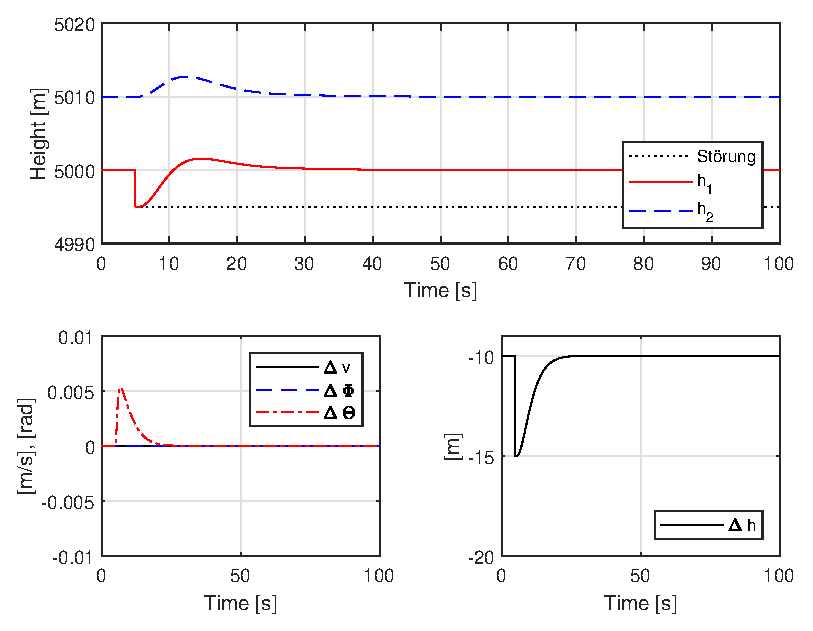
\includegraphics[width=\linewidth]{./Bilder/outputs_luftloch.eps}
 		\caption{Einfluss des Luftlochs auf die Höhe und die verkoppelten Ausgänge des nichtlinearen Modells}
 		\label{fig:outputs_luftloch}
 	\end{subfigure}
 	\hfill
 	\begin{subfigure}{.49\textwidth}
 		\centering
 		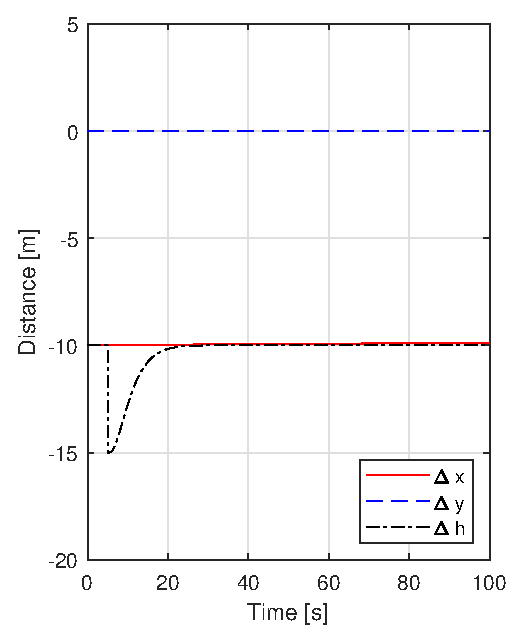
\includegraphics[width=0.65\linewidth]{./Bilder/distance_xyz_luftloch.eps}
 		\caption{Einfluss des Luftlochs auf die Positionsdifferenz der Flugzeuge beim nichtlinearen Modell}
 		\label{fig:distance_xyz_luftloch}
 	\end{subfigure}
 	\caption{Systemverhalten bei Störung durch ein Luftloch von \valunit{5}{m}}
 	\label{fig:luftloch}
 \end{figure}

\subsection{Störung durch Wind}
Störungen durch Windeinflüsse werden ebenfalls als sprungförmig modelliert. Dazu wird das in \Simulink\, implementierte Windmodell "Discrete Wind Gust Model \cite{windmodel}"\, verwendet, welches Windböen bezüglich der drei körperfesten Geschwindigkeitsachsen eines Flugzeugs erzeugt. Die Windböen nehmen dabei direkten Einfluss auf die Geschwindigkeit des Flugzeugs. Die Stärke der Windböen wird motiviert durch \cite{pollini} zu $\begin{bmatrix}
u_w, v_w, w_w
\end{bmatrix}^\transp = \begin{bmatrix}
0.5, 3.5, 0.5 
\end{bmatrix}^\transp$ \unit{m/s} gewählt - die Windböe wirkt also maßgeblich in Querrichtung der Flugzeuge. In diesem Fall wird angenommen, dass beiden Flugzeuge den Windböen gleichermaßen ausgesetzt sind. 
Die Windboe ist in Abbildung \ref{fig:windboe} gezeigt. Sie beginnt nach \valunit{10}{s}, ist über einen Zeitraum von \valunit{50}{s} konstant und klingt anschließend wieder ab.
 \begin{figure}[h] % figure störung windböe
	\centering
	\begin{subfigure}{.49\textwidth}
		\centering
		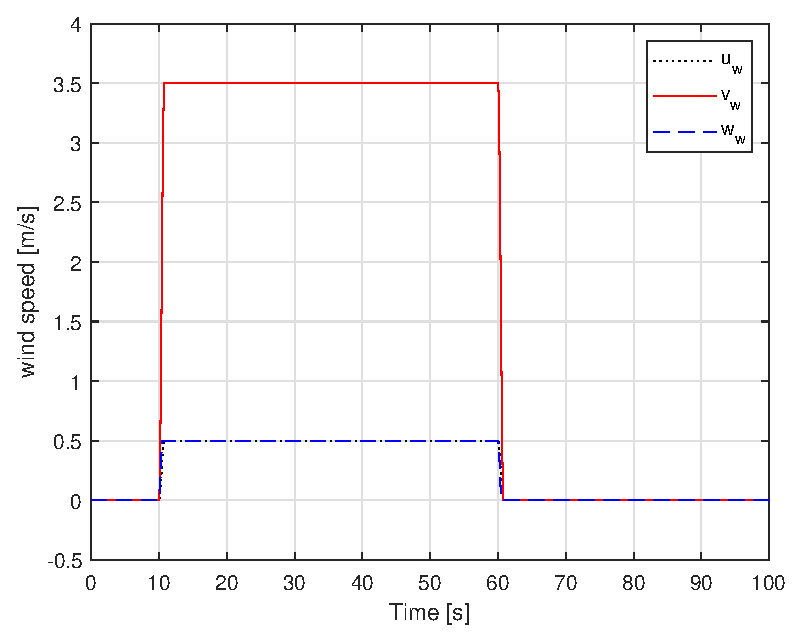
\includegraphics[width=\linewidth]{./Bilder/windboe.eps}
		\caption{Die drei Geschwindigkeitskomponenten der Windböe}
		\label{fig:windboe}
	\end{subfigure}
	\hfill
	\begin{subfigure}{.49\textwidth}
		\centering
		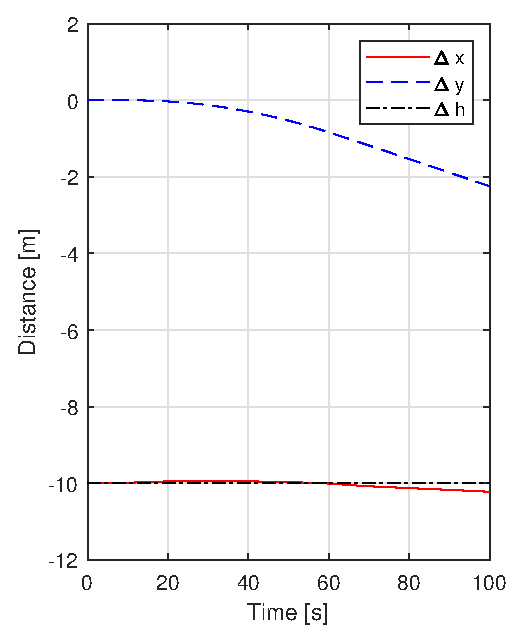
\includegraphics[width=0.65\linewidth]{./Bilder/distance_xyz_windboe.eps}
		\caption{Einfluss der Windböe auf die Positionsdifferenz der Flugzeuge beim nichtlinearen Modell}
		\label{fig:distance_xyz_windboe}
	\end{subfigure}
	\caption{Störung durch eine Windböe}
	\label{fig:pos_windboe}
\end{figure}

In Abbildung \ref{fig:outputs_windboe} ist das Systemverhalten unter Einfluss der Windstörung dargestellt. Abbildung \ref{fig:outputs_y1_windboe} zeigt den Einfluss auf die Höhen der Flugzeuge sowie den Einfluss auf die Ausgänge $v_1, \Phi_1$ und $\Theta_1$. Es ist deutlich erkennbar, dass die Windböe zu einem Auf- bzw. Abschwingen der einzelnen Größen führt. Die Flugzeuge schwingen in ihrer Höhe jeweils um \valunit{90}{cm}, wobei der Einfluss nach jeweils \valunit{20}{s} abgeklungen ist. Auch bei dieser Störung zeigt sich, dass Flugzeug 2 dem Verhalten von Flugzeug 1 im Sinne der Verkopplung folgt, obwohl für seine Ausgänge keine separate Unterlagerung entworfen wurde. Die Ausgänge $v_1, \Phi_1$ und $\Theta_1$ werden ebenfalls durch die Windböe beeinflusst und weichen von ihren Arbeitspunkten ab. Die Geschwindigkeitskomponente $v_1$ weicht um \valunit{0.18}{m/s} ab, wird jedoch nach \valunit{6}{s} zurück auf ihren Sollwert ausgeregelt. Die Abweichung bei $\Phi_1$ beträgt \valunit{0.025}{rad}, bei $\Theta_1$ \valunit{0.003}{rad}. Der Einfluss auf diese Größen ist damit äußerst gering. Es zeigt sich, dass die Windböe durch die Unterlagerung stationär genau ausgerelt wird. In Abbildung \ref{fig:outputs_ycoupl_windboe} ist der Einfluss auf die verkoppelten Ausgänge dargestellt. Auch hier ist gut zu erkennen, dass der Einfluss durch die Windböe marginal ist und die Verkopplung der einzelnen Größen, bis auf Abweichungen $<1\eexp{-03}$, erhalten bleibt.
\begin{figure}[H] % figure outputs windböe
	\centering
	\begin{subfigure}{0.49\textwidth}
		\centering
		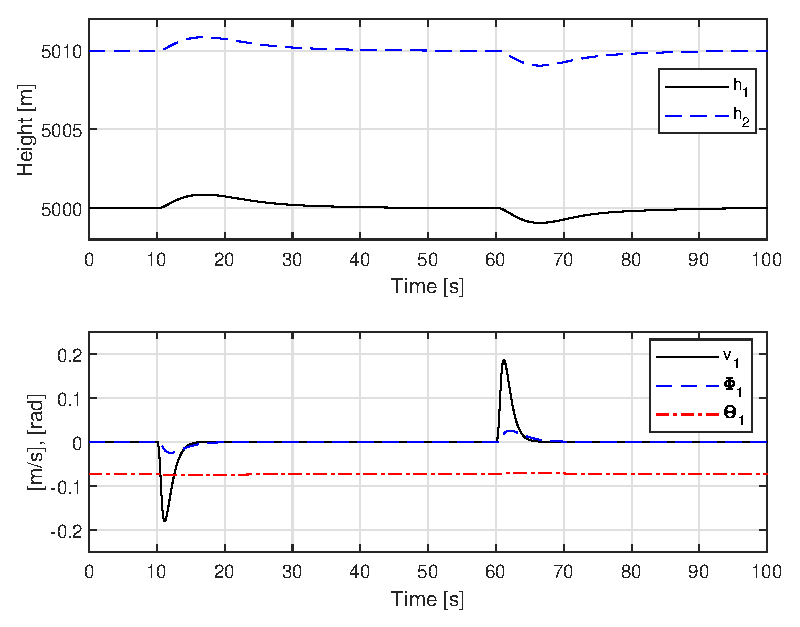
\includegraphics[width=\linewidth]{./Bilder/outputs_y1_windboe.eps}
		\caption{Einfluss der Windböe auf die Höhe der Flugzeuge 1 und 2 und die Ausgänge von Flugzeug 1 beim nichtlinearen Modell}
		\label{fig:outputs_y1_windboe}
	\end{subfigure}
	\hfill
	\begin{subfigure}{0.49\textwidth}
		\centering
		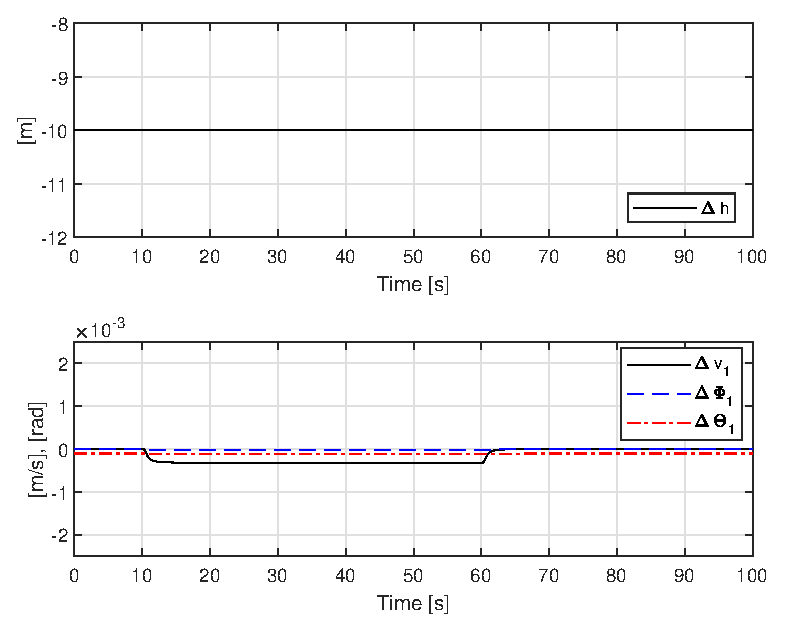
\includegraphics[width=\linewidth]{./Bilder/outputs_ycoupl_windboe.eps}
		\caption{Einfluss der Windböe auf die verkoppelten Ausgänge der Flugzeuge beim nichtlinearen Modell}
		\label{fig:outputs_ycoupl_windboe}
	\end{subfigure}
	\caption{Systemverhalten bei Störung durch eine Windböe}
	\label{fig:outputs_windboe}
\end{figure} 

Der Einfluss der Windböe auf die Positionsdifferenzen der Flugzeuge ist in Abbildung \ref{fig:distance_xyz_windboe} dargestellt. Trotz der Verkopplung der Ausgangsgrößen ist eine deutliche Abweichungen der Flugzeugpositionen zu erkennen. Sowohl in $x-$Richtung als auch in $y-$Richtung weichen die Positionen der Flugzeuge von einander ab. Während die Abweichung in $x-$Richtung relativ gering ist, beträgt die Abweichung in $y-$Richtung nach \valunit{100}{s} bereits über \valunit{2}{m}. Damit lässt sich schlussfolgern, dass die Windböe, welche auf beide Flugzeuge gleichermaßen einwirkt, zwar unter Beibehaltung der Verkopplung für die Ausgänge $v, \Phi, \Theta$ und $h$ stationär genau ausgeregelt wird. Die Verkopplung der Positionen ist allerdings bei Wirken der Störung nicht mehr gegeben, was daran liegt, dass die Positionen in der Regelschleife nicht enthalten sind.

\section{Probleme bei der Lösbarkeit des Optimierungsproblems mit \texttt{gammasyn}}
Wie bereits erläutert, wurde zur Regleroptimierung die \Matlab Toolbox \texttt{gammasyn} des IAT verwendet. Im Laufe dieses Projekts traten an mehreren Stellen immer wieder Fehler bei der Optimierung auf und führten zu unerwarteten Problemen. In diesem Abschnitt wird auf diese Fehler eingegangen. Zum einen soll dies der Transparenz der zum Reglerentwurf durchgeführten Schritte dienen. Zum anderen soll dies dazu dienen, Personen, die sich im Anschluss an dieses Projekt mit dem Thema beschäftigen, darauf aufmerksam zu machen, an welchen Stellen Probleme auftreten können und worin unter Umständen Verbesserungspotential für das Modell und die verwendeten Methoden besteht. Sofern nicht explizit anders erklärt, wurde für das Herbeiführen der hier beschriebenen Probleme nur das nominelle Modell verwendet.

\subsection{Entfernen kleiner Werte ($<\eexp{-09}$) aus den Matrizen}
Numerisch sehr kleine Werte, von denen man zunächst keine numerische Relevanz erwarten würde, \textbf{nicht} aus den Systemmatrizen \mat{A} und \mat{B} entfernt. Ein Entfernen dieser Werte führt in \texttt{gammasyn} bei ansonsten unveränderten Parametern zu einem Rangabfall in der Constraint Matrix und dadurch zu einem Fehler, was auf ein nicht lösbares Gleichungssystem hindeutet. 

In Kapitel \ref{cha:Regler} wurde ebenfalls erklärt, dass jene kleine Werte aus den Initialwerten $\mat{K}_\tn{init}$ und $\mat{F}_\tn{init}$ der Optimierung explizit entfernt wurden. Hier zeigte sich, dass gegenteiliges Vorgehen zwar zu einem erfolgreichen Entwurf führt, das Ergebnis jedoch stark von dem ursprünglichen Ergebnis abweicht. Es werden vollkommen andere Reglermatrizen $\mat{K}_\tn{koppel}$ und $\mat{F}_\tn{mod}$ erzielt, was zu anderen Pollagen führt. Das Systemverhalten dieser Regler führte auch bei der Führungsgröße $h_1$ zu enorm hohen Stellgrößen und damit zu instabilem Verhalten, weshalb diese Ergebnisse nicht weiter betrachtet wurden. 

Es lässt sich also insgesamt festhalten, dass je nach Startwert und Entfernen numerisch sehr kleiner Werte, mit dem in dieser Arbeit verwendeten Modell vollkommen verschiedene Ergebnisse, bis hin zu nicht lösbaren Optimierungsproblemen erzielt werden. 

\subsection{Variation des Arbeitspunktes}
Ähnlich zu der zuvor beschriebenen Abhängigkeit bezüglich der Startwerte, konnte festgestellt werden, dass auch eine Variation des Arbeitspunktes unter Umständen zu einem nicht lösbaren Gleichungssytem in der Optimierung führen kann. Wird beispielsweise die Geschwindigkeit der Flugzeuge im Arbeitspunkt von $u_{1\tn{AP}} = u_{2\tn{AP}} = \valunit{150}{m/s}$ auf $u_{1\tn{AP}} = u_{2\tn{AP}} = \valunit{130}{m/s}$ verringert, so lässt sich immer noch ein stabiler Arbeitspunkt für den Geradeausflug bestimmen. Allerdings schlägt die Optimierung auch hier wider Erwarten aufgrund eines nicht lösbaren Gleichungssystems fehl. Dies gilt sowohl für das ursprünglich verwendete Polgebiet, welches in Kapitel \ref{cha:Regler} erklärt wurde, als auch für Polgebiete, welche nur die Imaginärachse der komplexen s-Halbebene als Mindestanforderung besitzen oder Polgebiete, die sogar instabiles Verhalten zulassen.

\subsection{Parameterschwankung in der Masse bei Verwendung eines einzelnen Modells}
Ein weiterer Problemfall tritt auf, wenn anstelle des nominellen Modells eines der Modelle 2 (vor der Betankung) oder 3 (nach der Betankung) verwendet wird. Wenn man nun versucht einen Regler nur für Modell 2 unter Beibehaltung der Startwerte und des Polgebiets aus Kapitel \ref{cha:Regler} auszulegen, dann führt das gemäß der Erklärungen in Abschnitt \ref{sec:Parameterschwankungen} zu unterschiedlichen Arbeitspunkten für die beiden Flugzeuge. Wird nun die Treibstoffmasse über den Parameter $t\in[0,1]$ variiert, kann dies aufgrund von Rangfehlern zu einem nicht lösbaren Gleichungssystem bei der Optimierung führen. Nachfolgend werden dazu beispielhaft einige Werte für $t$ genannt, die zu lösbaren bzw. unlösbaren Gleichungssystemen führen.
\begin{table}[h]
\begin{center}
 \begin{tabular}{||c c c||} 
	\hline
	$t$ & lösbar & nicht lösbar \\ [0.5ex] 
	\hline
	0.1 & X & - \\
	0.5 & X & - \\
	0.8 & - & X \\
	0.9 & X & - \\
	1 & - & X \\
	1.1 & X & - \\
	1.3 & - & X \\
	1.4 & X & - \\
	\hline
\end{tabular}
\caption{\label{tab:parameterschwankung_t} Lösbarkeit des Gleichungssystems bei der Optimierung für Modell 2 in Abhängigkeit der Treibstoffmasse.}
\end{center}
\end{table} 
Tabelle \ref{tab:parameterschwankung_t} stellt dar, ob die Optimierung für Modell 2 bei entsprechender Wahl von $t$ für die Treibstoffmasse zu einem lösbaren oder nicht lösbaren Gleichungssystem innerhalb der Optimierung führt. Wie zu erkennen ist, gibt es keine eindeutige Abgrenzung, ab der der Massenunterschied der beiden Flugzeuge aufgrund des Treibstoffs zu groß wird. Viel mehr liegt hier die Vermutung nahe, dass die Lösbarkeit des Optimierungsproblems und damit auch die Tatsache, ob ein Verkopplungsregler für das System gefunden werden kann, stark von der Masse des Treibstoffs abhängt.

\subsection{Entfernen der Verkopplungsbedingung für $\Delta \Theta$}
Die Auswertung des linearen Modells hat bereits gezeigt, dass die Vorgabe von $\Theta_1$ mit dem Verkopplungsregler zu sehr hohen Stellgrößen und damit zu instabilem Verhalten führen kann, falls die Stellgrößen beschränkt werden. Dazu kommt die Vermutung, dass die Forderung zwei Flugzeuge, die unterschiedliche Massen und damit verschiedene Arbeitspunkte besitzen, sowohl in ihrer Höhe als auch in ihrem Nickwinkel miteinander zu verkoppeln, nur schwer umsetzbar ist. Die unterschiedlichen Massen führen dazu, dass das Systemverhalten der beiden Flugzeuge nicht mehr übereinstimmt. Eine Möglichkeit diese Problematik zu umgehen, ist der Ansatz die Verkopplungsbedingung für $\Delta \Theta$ zu entfernen und stattdessen $\Theta_2$ ebenfalls als Regelgröße einzuführen. Dieser Ansatz führt allerdings auch bereits bei der minimalen Forderung nach Stabilität zu einem Rangfehler in der Optimierung und damit zu einem nicht lösbaren Gleichungssystem.
	\chapter{Fazit und Ausblick}\label{chap:Fazit}
Nachdem die Ergebnisse ausführlich diskutiert wurden, sollen die Erkenntnisse der Arbeit im folgenden Abschnitt noch einmal zusammengefasst werden. Außerdem werden anhand der gewonnenen Ergebnisse einige Vorschläge für zukünftige Forschungsarbeiten gemacht.

\section{Zusammenfassung der Ergebnisse}
Zunächst lässt sich sagen, dass eine erfolgreiche Verkopplung am nominellen System durchgeführt werden kann. Hierbei zeigt sich jedoch, dass die Regelung bezogen auf den Nickwinkel $\Theta$ sehr empfindlich reagiert.
Diese Sensibilität äußert sich sowohl in den Stellgrößenverläufen als auch bei der Störgrößenrobustheit.

Bei der Untersuchung der Robustheit bezüglich Parameterschwankungen, zeigt sich, dass mithilfe des Multi-Modell-Ansatzes kein robuster Verkopplungsregler ausgelegt werden kann. Selbst bei Modellen mit nur geringen Massenunterschieden kommt es entweder zu numerischen Problemen oder die Optimierung führt zu instabilen Reglern - selbst wenn durch das Polgebiet lediglich Stabilität gefordert wird. 
Bei Verwendung des Reglers, welcher für das nominelle Modell ausgelegt wurde, führen Masseschwankungen zu bleibenden Regelabweichungen. Zudem werden die Verkopplungsbedingungen nicht mehr erfüllt und es kommt zu unerwünschten Abweichungen bei den relativen Positionen der Flugzeuge.
Die Robustheit gegenüber Masseschwankungen kann mit dem entworfenen Regler nicht erzielt werden.

Bezogen auf sprungförmige Störungen hingegen, lassen sich mit Hilfe der unterlagerten Regelung, bessere Ergebnisse erzielen. Es zeigt sich, dass es möglich ist, Störungen, welche direkt auf die Zustände wirken, auszuregeln. Bei der Störung durch Luftlöcher bleibt auch der Abstand zwischen den Flugzeugen konstant.
Beaufschlagt man jedoch Wind als Störung, so bleibt zwar die Verkopplung erhalten, bei den relative Flugzeugpositionen kommt es allerdings wieder zu unerwünschten Abweichungen, da die Positionsdifferenz nicht explizit geregelt wird.

\section{Ausblick für zukünftige Forschungsprojekte}
Für die Zukunft gilt es zunächst die aufgetretenen Probleme zu beheben. Hierfür sollte auf jeden Fall eine Erweiterung der Regelung um die Positionen der beiden Flugzeuge in $x$- und $y$-Richtung implementiert werden. Des Weiteren kann eine Trajektorien-Folge-Regelung dabei helfen vorgegebene Kurse abzufliegen.
Auch eine Verbesserung der Robustheit gilt es zu ermöglichen. Bezogen auf die Masse, könnte diese als zusätzlicher Zustand im Modell integriert werden, um Schwankungen beim Betankungsvorgang besser berücksichtigen zu können. Eine Überarbeitung des Modells oder eine Anpassung des Optimierungsalgorithmus könnten zu einer Verbesserung der numerischen Stabilität führen.

Zudem wird in dieser Arbeit davon ausgegangen, dass alle Zustandsgrößen exakt zur Verfügung stehen. Da dies in der Realität nicht der Fall sein wird, sollte eine Modellierung der Sensorik implementiert werden. Hierbei müssten Rauscheinflüsse und Dynamiken der Sensoren berücksichtigt werden. Des Weiteren sind Recherchen nötig, um zu klären welche Sensorsignale zur Verfügung stehen und welche eventuell geschätzt werden müssten. Diese Schätzungen könnten beispielsweise mit einem Beobachterentwurf geschehen. Außerdem wurde die Dynamik der Aktorik vernachlässigt. Um ein noch realitätsgetreueres Modell zu erhalten, kann die Dynamik der Stellglieder zusätzlich modelliert werden.

In vorliegender Arbeit wird der Einfachheit halber zunächst davon ausgegangen, dass es sich bei beiden Flugzeugen um das gleiche Modell handelt. Ein weiteres Forschungsgebiet stellt die explizite Gestaltung des Tankflugzeugs dar. Dieses muss speziell auf die Problematiken bei der Luftbetankung angepasst werden. Das heißt, es sollte zum Beispiel eine gewisse Dynamik aufweisen oder robuster auf Turbulenzen und Windböen reagieren. Mit einem für diesen Vorgang entsprechend angepassten Flugzeug, wäre es wahrscheinlich möglich, bessere Ergebnisse zu erzielen. Zudem kann der Detaillierungsgrad erhöht werden, indem der Einfluss der beiden Flugzeuge aufeinander berücksichtigt wird. 

Global betrachtet ist noch einiges an Forschung nötig bis erste Prototypen getestet werden können. Nichtsdestotrotz handelt es sich bei der zivilen Luftbetankung um einen vielversprechenden Ansatz, welcher bei einer zukünftigen, serienmäßigen Umsetzung enorme Mengen an Kraftstoff einsparen wird. Dies wäre ein weiterer Schritt hin zu einer klimaneutralen Gesellschaft.

%- Modell vallidiert\\
%- Verkopplung für Nominelles System gelungen\\
%- Leider numerische Probleme evt. behebar durch weiter forschung\\
%
%
%
%-Verkopplung für lin un NL Modell erfolgreich\\
%
%-Sobald stellgr.beschr. dann mit Theta instab\\
%-restl. Stellgr. eingehalten\\
%- für alle ausser Theta auch pos. verkopplung bei führungsgr. sprüngen \\
%- Multi Modell failt auch schon für extrem klein schwankungen\\
%	-> Verkoppll nichtmerh möglich, system instabil weil EW rechts also lnicht robust\\
%zeigt sich auch wenn man die Modell mit Massenschwankungen mit unserem regeler regelt (der fürs nominelle ohne Multi) dann regelabweichung, verkopplun gnihct ewrfüllt und pos. weicht ab\\
%
%-> Keine robustheit gegenüber Masseschwankungen\\
%
%- unterlagerung kann sprungförmige strörungen ausregeln\\
%-luftloch bleibt verkopplung erhalten(auch in Pos.)\\
%- bei Wind bleibt verkopplung der ausgänge erhalten aber nicht bei POs.\\
%
%-> robust gegen störungen die direkt auf Zustände wirken\\
%-> Pos. verkopplung kann nicht erreicht werden.\\









%Ausblick \\
%
%-Modellierung der parameterschwankung Masse\\
%- Modellierung von Sensoren\\
%- Evtl. implementierung einer Trajektorienfolgeregelung \\
%
%Weitere Forschung dann erste Prototypen zur praktischen erprobung -> wird noch dauern bis Serienmäßig 
%Dennoch vielversprechender Ansatz welcher bei Umsetzung enorme Menge Kraftstoff einsparen wird und damit einen Schritt weiter \\
%
%-Unterschiedliche Flugzeuge Modellieren -> andere Dynamik\\
%-Erweiterung der Regulung um Pos. regelung (Verkopplung von xyz)\\
%-Modellierung der Sensorik\\
%-Verbesserung der Robustheit (gegenüber masseschw., Abhängigkeit AP, Abh. Nummerik)\\
%-evtl.(verbesserung Rob -> krasse Theta Abh. -> Verk ohne Theta)\\
%- evtl. (warum ist gammasyn so kacke)\\



	% =================================================================================
	% Anhang
	% =================================================================================
	\appendix % Damit wird der Anhang begonnen. Die Kapitel werden ab jetzt mit Buchstaben nummeriert
	
	\chapter{Regler- und Systemmatrizen}\label{app:matrizen}
Die Systemmatrizen für das nominelle System lauten
\begin{equation*}
\textbf{A} = \begin{bmatrix} 
-0.0426 & 0 & -0.008282 & 0 & 10.81 & 0 & 0 & -9.784 & 0.0003409\\ 
0 & -0.208 & 0 & -11.02 & 0 & -150.0 & 9.784 & 0 & 0\\
-0.1844 & 0 & -0.7339 & 0 & 147.1 & 0 & 0 & 0.7189 & 0.001059\\
0 & -0.09575 & 0 & -4.888 & 0 & 2.321 & 0 & 0 & 0\\
-0.002906 & 0 & -0.02645 & 0 & -1.143 & 0 & 0 & 0 & 7.811e-6\\
0 & 0.03642 & 0 & 0.4039 & 0 & -2.089 & 0 & 0 & 0\\
0 & 0 & 0 & 1.0 & 0 & -0.07348 & 0 & 0 & 0\\ 
0 & 0 & 0 & 0 & 1.0 & 0 & 0 & 0 & 0\\ 
-0.07329 & 0 & -0.9973 & 0 & 0 & 0 & 0 & 150.4 & 0 \\
\end{bmatrix}
\end{equation*}

\begin{equation*}
\textbf{B} = \begin{bmatrix}
-1.009 & 9.81 & 0 & 0\\ 0 & 0 & 0 & 4.329\\ -13.73 & 0 & 0 & 0\\ 0 & 0 & -6.056 & 2.354\\ -5.333 & 0.2912 & 0 & 0\\ 0 & 0 & 0.1267 & -2.596\\ 0 & 0 & 0 & 0\\ 0 & 0 & 0 & 0\\ 0 & 0 & 0 & 0 \\
\end{bmatrix}.
\end{equation*}
Numerisch sehr kleine Werte $<10^{-09}$ werden aus Gründen der numerischen Stabilität nicht aus den Systemmatrizen entfernt. Für die Reglermatrizen gilt das Gegenteil. Da wie bereits zuvor erwähnt das Entfernen von sehr kleinen Werten $<10^{-09}$ aus den Reglermatrizen unerwarteter Weise zu numerischen Berechnungsproblemen und damit zu Optimierungsabbrüchen führt, werden diese nicht entfernt.
\begin{equation*}
\mat{F}_\tn{mod} = 
\begin{bmatrix}
1.8102\eexp{-13} & 1.5337\eexp{-13} & -171.2109 & 4.4174\eexp{-04}; \\
3.0748\eexp{-12} & 3.4751\eexp{-12} & -3111.7757 & 0.0320; \\
0.1382 & -0.9011 & 4.7167\eexp{-12} & -1.3999\eexp{-14}; \\
0.3295 & -1.3869\eexp{-13} & -8.5272\eexp{-12} & -8.3947\eexp{-14}; \\
-5.5453\eexp{-13} & 2.3767\eexp{-13} & -166.1567 & 3.8831\eexp{-04}; \\
-1.0261\eexp{-11} & 5.1066\eexp{-12} & -3015.8835 & 0.0310; \\
0.1383 & -0.9021 & 5.8368\eexp{-12} & -1.3996\eexp{-14}; \\
0.3299 & -1.3906\eexp{-13} & -8.6262\eexp{-12} & -8.4039\eexp{-14}
\end{bmatrix}
\end{equation*}

\begin{equation*}
\mat{K}_\tn{koppel} = 
\begin{bmatrix}
0.2181 & 1.3670\eexp{-07} & -0.0101 & -6.6039\eexp{-09} & ... \\
-0.6069 & 4.8960\eexp{-10} & 3.5613\eexp{-08} & -1.3294 & ... \\
-0.0013 & 1.1667\eexp{-05} & -1.3670\eexp{-07} & 1.5900\eexp{-04} & ... \\
6.6050\eexp{-09} & 2.7366\eexp{-04} & -4.8759\eexp{-10} & -3.5613\eexp{-08} & ... \\
5.5512\eexp{-04} & 5.2847\eexp{-05}; & & \\ 
3.9833 & -7.5467\eexp{-09} & -0.2863 & 3.8470\eexp{-10} & ... \\ 
0.0357 & 5.0982\eexp{-11} & -1.9650\eexp{-09} & 0.1041 & ... \\
-7.4242\eexp{-04} & 4.0686\eexp{-04} & 7.5498\eexp{-09} & 0.0055 & ... \\
-3.6007\eexp{-10} & 2.8206\eexp{-04} & -2.4985\eexp{-11} & 1.9668\eexp{-09} & ... \\
0.0066 & 2.3179\eexp{-04}; & & \\ 
1.06151\eexp{-09} & 0.1294 & 1.444\eexp{-08} & -1.7276 & ... \\
1.0361\eexp{-10} & -14.8366 & -0.0207 & -7.6591\eexp{-11} & ... \\
1.0636\eexp{-07} & -1.0599\eexp{-09} & 0.0048 & -1.4445\eexp{-08} & ... \\
0.0616 & -1.0366\eexp{-10} & -0.0045 & 0.0677 & ... \\
5.9533\eexp{-11} & -1.0636\eexp{-07}; & & \\
-7.6565\eexp{-10} & 0.4811 & -1.0419\eexp{-08} & -2.4372 & ... \\
3.1464\eexp{-11} & -34.6613 & 1.3199 & -3.5873\eexp{-11} & ... \\
-3.6855\eexp{-08} & 7.6455\eexp{-10} & -0.1995 & 1.0419\eexp{-08} & ... \\
-0.1092 & -3.1506\eexp{-11} & 0.0080 & 0.94028 & ... \\
4.7949\eexp{-11} & 3.6855\eexp{-08}; & & \\
-3.0300\eexp{-05} & -1.3665\eexp{-07} & -4.1234\eexp{-04} & 6.5917\eexp{-09} & ... \\
-3.3363\eexp{-04} & -4.8802\eexp{-10} & -3.5574\eexp{-08} & -5.76058\eexp{-04} & ... \\
5.3260\eexp{-05} & 0.2115 & 1.3665\eexp{-07} & -0.0102 & ... \\
-6.5912\eexp{-09} & -0.6073 & 4.8487\eexp{-10} & 3.5574\eexp{-08} & ... \\
-1.3312 & -0.0013; & & \\ 
-4.0613\eexp{-04} & 7.5514\eexp{-09} & -0.0055 & -3.6580\eexp{-10} & ... \\
-2.8814\eexp{-04} & -3.6877\eexp{-11} & 1.9671\eexp{-09} & -0.0068 & ... \\
2.5437\eexp{-04} & 3.8598 & -7.5616\eexp{-09} & -0.2879 & ... \\
3.7587\eexp{-10} & 0.0352 & -3.9288\eexp{-12} & -1.9660\eexp{-09} & ... \\
0.0907 & -7.5648\eexp{-04}; & & \\ 
-1.0601\eexp{-09} & 0.0048 & -1.4426\eexp{-08} & 0.0611 & ... \\
-1.0270\eexp{-10} & -0.0044 & 0.0676 & 7.6570\eexp{-11} & ... \\
-1.0624\eexp{-07} & 1.0585\eexp{-09} & 0.1295 & 1.4426\eexp{-08} & ... \\
-1.7282 & 1.0265\eexp{-10} & -14.8511 & -0.0207 & ... \\
-5.9604\eexp{-11} & 1.0624\eexp{-07}; & & \\ 
7.6471\eexp{-10} & -0.1990 & 1.0406\eexp{-08} & -0.1090 & ... \\
-3.1093\eexp{-11} & 0.0080 & 0.9415 & 3.5545\eexp{-11} & ... \\
3.6809\eexp{-08} & -7.6361\eexp{-10} & 0.4809 & -1.0407\eexp{-08} & ... \\
-2.4364 & 3.1097\eexp{-11} & -34.6993 & 1.3211 & ... \\\\
-4.7764\eexp{-11} & -3.6809\eexp{-08} & &
\end{bmatrix}
\end{equation*}
	
%	\input{./inc/commonmacros_desc.tex}
	
%	\ifSADAfinal
%		\SADApostfacelof  % Abbildungsverzeichnis
%		\SADApostfacelot  % Liste der Tabellen
%		\SADApostfaceloa  % Liste der Algorithmenür Paket algorithm
%		\SADApostfacelol  % Liste der Listings
%		\SADApostfacebib{}{} % Literaturverzeichnis Argumente nur für BibTex notwendig. 1. Argument: Stil   2. Argument .bib Datei
	
%		\SADApostface[
%			lof=false,
%			lot=false,
%			loa=false,
%			lol=false,
%			bib=true,
%			order={lof,lot,bib},
%			bibstyle=bababbrv,
%			bibfile=./bib/literature
%		]
%	\fi
	\printbibliography
\end{document}